% Options for packages loaded elsewhere
% Options for packages loaded elsewhere
\PassOptionsToPackage{unicode}{hyperref}
\PassOptionsToPackage{hyphens}{url}
\PassOptionsToPackage{dvipsnames,svgnames,x11names}{xcolor}
%
\documentclass[
  letterpaper,
  11pt,
  english,
  singlespacing,
  headsepline,
  openany]{MastersDoctoralThesis}
\usepackage{xcolor}
\usepackage[paper=a4paper,inner=2.5cm,outer=3.8cm,bindingoffset=.5cm,top=1.5cm,bottom=1.5cm]{geometry}
\usepackage{amsmath,amssymb}
\setcounter{secnumdepth}{5}
\usepackage{iftex}
\ifPDFTeX
  \usepackage[T1]{fontenc}
  \usepackage[utf8]{inputenc}
  \usepackage{textcomp} % provide euro and other symbols
\else % if luatex or xetex
  \usepackage{unicode-math} % this also loads fontspec
  \defaultfontfeatures{Scale=MatchLowercase}
  \defaultfontfeatures[\rmfamily]{Ligatures=TeX,Scale=1}
\fi
\usepackage{lmodern}
\ifPDFTeX\else
  % xetex/luatex font selection
\fi
% Use upquote if available, for straight quotes in verbatim environments
\IfFileExists{upquote.sty}{\usepackage{upquote}}{}
\IfFileExists{microtype.sty}{% use microtype if available
  \usepackage[]{microtype}
  \UseMicrotypeSet[protrusion]{basicmath} % disable protrusion for tt fonts
}{}
\makeatletter
\@ifundefined{KOMAClassName}{% if non-KOMA class
  \IfFileExists{parskip.sty}{%
    \usepackage{parskip}
  }{% else
    \setlength{\parindent}{0pt}
    \setlength{\parskip}{6pt plus 2pt minus 1pt}}
}{% if KOMA class
  \KOMAoptions{parskip=half}}
\makeatother
% Make \paragraph and \subparagraph free-standing
\makeatletter
\ifx\paragraph\undefined\else
  \let\oldparagraph\paragraph
  \renewcommand{\paragraph}{
    \@ifstar
      \xxxParagraphStar
      \xxxParagraphNoStar
  }
  \newcommand{\xxxParagraphStar}[1]{\oldparagraph*{#1}\mbox{}}
  \newcommand{\xxxParagraphNoStar}[1]{\oldparagraph{#1}\mbox{}}
\fi
\ifx\subparagraph\undefined\else
  \let\oldsubparagraph\subparagraph
  \renewcommand{\subparagraph}{
    \@ifstar
      \xxxSubParagraphStar
      \xxxSubParagraphNoStar
  }
  \newcommand{\xxxSubParagraphStar}[1]{\oldsubparagraph*{#1}\mbox{}}
  \newcommand{\xxxSubParagraphNoStar}[1]{\oldsubparagraph{#1}\mbox{}}
\fi
\makeatother


\usepackage{longtable,booktabs,array}
\usepackage{calc} % for calculating minipage widths
% Correct order of tables after \paragraph or \subparagraph
\usepackage{etoolbox}
\makeatletter
\patchcmd\longtable{\par}{\if@noskipsec\mbox{}\fi\par}{}{}
\makeatother
% Allow footnotes in longtable head/foot
\IfFileExists{footnotehyper.sty}{\usepackage{footnotehyper}}{\usepackage{footnote}}
\makesavenoteenv{longtable}
\usepackage{graphicx}
\makeatletter
\newsavebox\pandoc@box
\newcommand*\pandocbounded[1]{% scales image to fit in text height/width
  \sbox\pandoc@box{#1}%
  \Gscale@div\@tempa{\textheight}{\dimexpr\ht\pandoc@box+\dp\pandoc@box\relax}%
  \Gscale@div\@tempb{\linewidth}{\wd\pandoc@box}%
  \ifdim\@tempb\p@<\@tempa\p@\let\@tempa\@tempb\fi% select the smaller of both
  \ifdim\@tempa\p@<\p@\scalebox{\@tempa}{\usebox\pandoc@box}%
  \else\usebox{\pandoc@box}%
  \fi%
}
% Set default figure placement to htbp
\def\fps@figure{htbp}
\makeatother


% definitions for citeproc citations
\NewDocumentCommand\citeproctext{}{}
\NewDocumentCommand\citeproc{mm}{%
  \begingroup\def\citeproctext{#2}\cite{#1}\endgroup}
\makeatletter
 % allow citations to break across lines
 \let\@cite@ofmt\@firstofone
 % avoid brackets around text for \cite:
 \def\@biblabel#1{}
 \def\@cite#1#2{{#1\if@tempswa , #2\fi}}
\makeatother
\newlength{\cslhangindent}
\setlength{\cslhangindent}{1.5em}
\newlength{\csllabelwidth}
\setlength{\csllabelwidth}{3em}
\newenvironment{CSLReferences}[2] % #1 hanging-indent, #2 entry-spacing
 {\begin{list}{}{%
  \setlength{\itemindent}{0pt}
  \setlength{\leftmargin}{0pt}
  \setlength{\parsep}{0pt}
  % turn on hanging indent if param 1 is 1
  \ifodd #1
   \setlength{\leftmargin}{\cslhangindent}
   \setlength{\itemindent}{-1\cslhangindent}
  \fi
  % set entry spacing
  \setlength{\itemsep}{#2\baselineskip}}}
 {\end{list}}
\usepackage{calc}
\newcommand{\CSLBlock}[1]{\hfill\break\parbox[t]{\linewidth}{\strut\ignorespaces#1\strut}}
\newcommand{\CSLLeftMargin}[1]{\parbox[t]{\csllabelwidth}{\strut#1\strut}}
\newcommand{\CSLRightInline}[1]{\parbox[t]{\linewidth - \csllabelwidth}{\strut#1\strut}}
\newcommand{\CSLIndent}[1]{\hspace{\cslhangindent}#1}



\setlength{\emergencystretch}{3em} % prevent overfull lines

\providecommand{\tightlist}{%
  \setlength{\itemsep}{0pt}\setlength{\parskip}{0pt}}



 


% \usepackage[utf8]{inputenc} % Required for inputting international characters
%\usepackage[T1]{fontenc} % Output font encoding for international characters; causes problems for xelatex

%\usepackage{mathpazo} % Use the Palatino font by default

%\usepackage[backend=bibtex, style=authoryear, natbib=true]{biblatex} % Use the bibtex backend with the authoryear citation style (which resembles APA)

%\usepackage[autostyle=true]{csquotes} % Required to generate language-dependent quotes in the bibliography

\setlength{\parindent}{2em}   % Einrückung
\setlength{\parskip}{0pt}

%----------------------------------------------------------------------------------------
%	MARGINS
%----------------------------------------------------------------------------------------

\geometry{
	headheight=4ex,
	includehead,
	includefoot
}

\raggedbottom

\AtBeginDocument{
\hypersetup{pdftitle=\ttitle} % Set the PDF's title to your title
\hypersetup{pdfauthor=\authorname} % Set the PDF's author to your name
\hypersetup{pdfkeywords=\keywordnames} % Set the PDF's keywords to your keywords
}
\usepackage{booktabs}
\usepackage{longtable}
\usepackage{array}
\usepackage{multirow}
\usepackage{wrapfig}
\usepackage{float}
\usepackage{colortbl}
\usepackage{pdflscape}
\usepackage{tabu}
\usepackage{threeparttable}
\usepackage{threeparttablex}
\usepackage[normalem]{ulem}
\usepackage{makecell}
\usepackage{xcolor}
\usepackage{enumitem}
\setlist[itemize]{label=--}
\usepackage{tabularx}
\renewcommand{\arraystretch}{1.2}
\captionsetup{width=\textwidth}
\makeatletter
\@ifpackageloaded{bookmark}{}{\usepackage{bookmark}}
\makeatother
\makeatletter
\@ifpackageloaded{caption}{}{\usepackage{caption}}
\AtBeginDocument{%
\ifdefined\contentsname
  \renewcommand*\contentsname{Table of contents}
\else
  \newcommand\contentsname{Table of contents}
\fi
\ifdefined\listfigurename
  \renewcommand*\listfigurename{List of Figures}
\else
  \newcommand\listfigurename{List of Figures}
\fi
\ifdefined\listtablename
  \renewcommand*\listtablename{List of Tables}
\else
  \newcommand\listtablename{List of Tables}
\fi
\ifdefined\figurename
  \renewcommand*\figurename{Figure}
\else
  \newcommand\figurename{Figure}
\fi
\ifdefined\tablename
  \renewcommand*\tablename{Table}
\else
  \newcommand\tablename{Table}
\fi
}
\@ifpackageloaded{float}{}{\usepackage{float}}
\floatstyle{ruled}
\@ifundefined{c@chapter}{\newfloat{codelisting}{h}{lop}}{\newfloat{codelisting}{h}{lop}[chapter]}
\floatname{codelisting}{Listing}
\newcommand*\listoflistings{\listof{codelisting}{List of Listings}}
\makeatother
\makeatletter
\makeatother
\makeatletter
\@ifpackageloaded{caption}{}{\usepackage{caption}}
\@ifpackageloaded{subcaption}{}{\usepackage{subcaption}}
\makeatother
\usepackage{bookmark}
\IfFileExists{xurl.sty}{\usepackage{xurl}}{} % add URL line breaks if available
\urlstyle{same}
\hypersetup{
  pdftitle={Handling Missing Data in Multilevel Models with Few Clusters: A Simulation Study},
  pdfauthor={Lona Frießner},
  colorlinks=true,
  linkcolor={blue},
  filecolor={Maroon},
  citecolor={black},
  urlcolor={blue},
  pdfcreator={LaTeX via pandoc}}


\thesistitle{Handling Missing Data in Multilevel Models with Few
Clusters: A Simulation
Study} % Your thesis title, this is used in the title and abstract, print it elsewhere with \ttitle
\supervisor{} % Your supervisor's name, this is used in the title page, print it elsewhere with \supname
\examiner{} % Your examiner's name, this is not currently used anywhere in the template, print it elsewhere with \examname
\degree{Master of
Science} % Your degree name, this is used in the title page and abstract, print it elsewhere with \degreename
\author{Lona
Frießner} % Your name, this is used in the title page and abstract, print it elsewhere with \authorname
\addresses{} % Your address, this is not currently used anywhere in the template, print it elsewhere with \addressname

\subject{} % Your subject area, this is not currently used anywhere in the template, print it elsewhere with \subjectname
\keywords{} % Keywords for your thesis, this is not currently used anywhere in the template, print it elsewhere with \keywordnames
\university{University of
Hamburg} % Your university's name, this is used in the title page and abstract, print it elsewhere with \univname
\department{Quantitative
Methods} % Your department's name, this is used in the title page and abstract, print it elsewhere with \deptname
\group{Institute of
Psychology} % Your research group's name and URL, this is used in the title page, print it elsewhere with \groupname
\faculty{Faculty of Psychology and Human Movement
Science} % Your faculty's name and URL, this is used in the title page and abstract, print it elsewhere with \facname

\setcounter{tocdepth}{1} % The depth to which the document sections are printed to the table of contents
\begin{document}
\frontmatter % Use roman page numbering style (i, ii, iii, iv...) for the pre-content pages

\pagestyle{plain} % Default to the plain heading style until the thesis style is called for the body content

%----------------------------------------------------------------------------------------
%	TITLE PAGE
%----------------------------------------------------------------------------------------

\begin{titlepage}
\begin{center}

\vspace*{.06\textheight}
{\scshape\LARGE \univname\par}\vspace{1.5cm} % University name
\textsc{\Large Master Thesis}\\[0.5cm] % Thesis type

\HRule \\[0.4cm] % Horizontal line
{\huge \bfseries \ttitle\par}\vspace{0.4cm} % Thesis title
\HRule \\[1.5cm] % Horizontal line
 
\begin{minipage}[t]{0.4\textwidth}
\begin{flushleft} \large
\emph{Author:}\\
\authorname
\end{flushleft}
\end{minipage}
\begin{minipage}[t]{0.4\textwidth}
\begin{flushright} \large
\emph{Supervisors:}\\
Prof.~Dr.~Simon Grund \\
Mark Lustig\end{flushright}
\end{minipage}\\[3cm]
 
\vfill


\groupname\\
\deptname\\[2cm] % Research group name and department name
 
\vfill

\includegraphics[height=3cm]{images/logo.png} % University/department logo

{\large Submission date: May 05, 2026}\\[4cm] % Date

 
\vfill
\end{center}
\end{titlepage}

%----------------------------------------------------------------------------------------
%	DECLARATION PAGE
%----------------------------------------------------------------------------------------


%----------------------------------------------------------------------------------------
%	ABSTRACT PAGE
%----------------------------------------------------------------------------------------

\begin{abstract}
\addchaptertocentry{\abstractname} % Add the abstract to the table of contents
Multilevel studies often involve two challenges simultaneously: small
numbers of clusters and missing data. However, the performance of modern
missing-data methods under these combined conditions remains
insufficiently understood, particularly in models with missing predictor
variables and contextual effects. This thesis examines the performance
of multiple imputation, using both conventional and
small-sample-corrected degrees of freedom, and compares it with a fully
Bayesian approach in a simulation study. The study features a simple
random-intercept model with a manifest group-mean predictor, with
missings in the predictor variable and one level-2 auxiliary variable.
Simulation conditions varied in terms of intraclass correlation (.1
vs.~.3), missingness mechanism (MAR vs.~MCAR), between-group effect size
(0 vs.~0.4), and level-2 sample size (15, 30, 60). Method performance
was evaluated in terms of bias, coverage, standard deviation of point
estimates, and interval width. Results indicate a trade-off between bias
and interval width for the between-group effect: multiple imputation
tended to produce more biased estimates, particularly under low
intraclass correlation conditions, whereas the Bayesian approach yielded
wider credible intervals. As coverage under conventional degrees of
freedom was already close to the nominal level, the small-sample
correction tended to result in overcoverage. The findings are discussed
with regard to methodological limitations and their implications for
applied multilevel research.
\end{abstract}



% 

\begingroup
\hypersetup{linkcolor=black}

\tableofcontents % Prints the main table of contents

\listoffigures % Prints the list of figures

\listoftables % Prints the list of tables

\endgroup






%----------------------------------------------------------------------------------------
%	THESIS CONTENT - CHAPTERS
%----------------------------------------------------------------------------------------

\mainmatter % Begin numeric (1,2,3...) page numbering

\pagestyle{thesis} % Return the page headers back to the "thesis" style
% Define some commands to keep the formatting separated from the content 
\newcommand{\keyword}[1]{\textbf{#1}}
\newcommand{\tabhead}[1]{\textbf{#1}}
\newcommand{\code}[1]{\texttt{#1}}
\newcommand{\file}[1]{\texttt{\bfseries#1}}
\newcommand{\option}[1]{\texttt{\itshape#1}}


\bookmarksetup{startatroot}

\chapter{Introduction}\label{introduction}

Multilevel models are a standard statistical tool for analyzing
clustered data, which frequently occur in the social sciences (e.g.,
patients nested within therapists, students within classes, or employees
within firms). In practice, such data sets are often characterized by a
relatively small number of groups and by the presence of missing values
(\citeproc{ref-maashox}{Maas \& Hox, 2005};
\citeproc{ref-mcneishstaple14}{McNeish \& Stapleton, 2016b};
\citeproc{ref-nicholson}{Nicholson et al., 2017};
\citeproc{ref-peugh}{Peugh \& Enders, 2004}).

Methodological research has proposed a range of approaches to address
each of these challenges separately. Small-sample corrections for
multilevel models have been developed to improve statistical inference
when the number of clusters is limited (\citeproc{ref-elff}{Elff et al.,
2021}; \citeproc{ref-holtmann}{Holtmann et al., 2016};
\citeproc{ref-mcneishstaple14}{McNeish \& Stapleton, 2016b},
\citeproc{ref-mcneish}{2016a}). At the same time, modern missing-data
methods have been extended to multilevel data structures (see e.g.
\citeproc{ref-audigier}{Audigier et al., 2018};
\citeproc{ref-enders16}{Enders et al., 2016};
\citeproc{ref-endersupdate}{Enders, 2025}; \citeproc{ref-grundapa}{Grund
et al., 2019}; \citeproc{ref-kahan}{Kahan et al., 2016};
\citeproc{ref-yucel}{Yucel, 2008}).

Some research has investigated how these two challenges interact, both
for single-level regressions (see e.g. \citeproc{ref-mcneish17}{McNeish,
2017a}; \citeproc{ref-hippel}{Von Hippel, 2013}) and in multilevel
contexts (e.g., \citeproc{ref-mcneishgrowth}{McNeish, 2018};
\citeproc{ref-shin}{Shin et al., 2025}; \citeproc{ref-shinshin}{Shin \&
Shin, 2025}; \citeproc{ref-zitzmann}{Zitzmann et al., 2015}). However,
the existing literature remains limited, particularly for multilevel
models in which effects of level-2 variables are of substantive
interest. Such level-2 variables may be directly measured group
characteristics (e.g., class size) or level-1 variables that are
included to estimate contextual effects, such as the mean cognitive
ability of students in a class (\citeproc{ref-croon}{Croon \& Van
Veldhoven, 2007}; \citeproc{ref-luedtkecontext}{Lüdtke et al., 2008};
\citeproc{ref-raudenbush}{Raudenbush \& Bryk, 2010};
\citeproc{ref-snijders}{Snijders \& Bosker, 2012}). Contextual models
are widely used in psychological research (e.g.,
\citeproc{ref-anderman}{Anderman, 2002};
\citeproc{ref-sport}{Papaioannou et al., 2004}), but missing data become
especially relevant in this setting. Incomplete predictor variables
generally pose additional challenges for statistical inference compared
to situations in which only the outcome variable is incomplete
(\citeproc{ref-bartlett}{Bartlett et al., 2015};
\citeproc{ref-endersbook}{Enders, 2022}). Additionally, in models with
manifest group means, previous work suggests that likelihood-based
approaches to incomplete predictors may produce biased estimates of
between-group effects (\citeproc{ref-grundapa}{Grund et al., 2019}),
which can make alternative approaches such as fully Bayesian estimation
and multiple imputation more appealing in such settings.

This thesis therefore investigates the suitability of modern approaches
to handling missing data in small-sample multilevel models with
contextual effects in which predictor variables are partially missing.
Specifically, the performance of multiple imputation and fully Bayesian
estimation is evaluated. The structure of this thesis is as follows:
First, the theoretical foundations of multilevel models are introduced,
and current methodological approaches for handling small samples and
missing data are reviewed. Subsequently, a simulation study is conducted
to investigate the performance of these methods under different data
conditions. Finally, the findings are discussed with regard to their
implications for handling missing predictor data in small-sample
multilevel models, and the limitations of the study are considered.

\bookmarksetup{startatroot}

\chapter{Theory}\label{theory}

\section{Theoretical foundation of multilevel
models}\label{theoretical-foundation-of-multilevel-models}

Populations in which units of interest (e.g., students, employees, or
musicians) are grouped into higher-level units such as classes, firms,
or ensembles, are common in the social sciences. Imagine, for example,
that you are interested in the musical self-concept of young adults and
whether it is related to how many hours they practice their instrument
each week. To investigate this question, you collect data from several
youth ensembles. You recruit 15 ensembles, each consisting of 10
players. Every player completes a questionnaire assessing their musical
self-concept as well as their weekly practice time. At first glance,
this seems like a simple data set of 150 individuals. At closer
inspection, however, players from the same ensemble rehearse together,
share teachers, and experience similar social and musical environments.
Their responses may therefore be more similar within ensembles than
between ensembles.

Data of this kind are called \emph{nested} or \emph{clustered}
(\citeproc{ref-snijders}{Snijders \& Bosker, 2012, p. 7}). Such data for
example arises from a multistage sampling process, in which groups are
sampled first and individuals are subsequently sampled within these
groups\footnote{In this thesis, the terms `groups' or `clusters' refer
  to higher-level units, while lower-level units are referred to as
  `persons', `individuals' or `observations'. These models can also be
  applied to longitudinal data, where measurement occasions are nested
  within individuals, and to data structures with more than two levels.}.
This process induces dependencies in the data, as observations within
the same group are not selected independently
(\citeproc{ref-snijders}{Snijders \& Bosker, 2012, p. 7}). Beyond the
sampling process, individuals within a group typically share contextual
influences (e.g., the same ensemble teacher or classroom environment),
which leads to increased similarity in their responses compared to
individuals from another group. As a consequence, the assumption of
independent errors in traditional linear models is violated, because
residuals within groups are correlated
(\citeproc{ref-raudenbush}{Raudenbush \& Bryk, 2010}). A widely used
approach to account for this structure is the use of \emph{multilevel
models} (also referred to as \emph{hierarchical linear models} or
\emph{mixed models}), which are introduced in the following section.

\subsection{The concept of multilevel regression
models}\label{the-concept-of-multilevel-regression-models}

The aim of regression analysis, whether single- or multilevel, is to
explain variance in an outcome variable by including associated
variables in the model as predictors (\citeproc{ref-snijders}{Snijders
\& Bosker, 2012, p. 80}). In single-level regression, the residual
\(e_{i}\) captures the unexplained variance in \(Y\), that is
differences in the outcome from the prediction that the model made
(\citeproc{ref-leonhart}{Leonhart, 2013, p. 319}). To account for the
dependency of the observations within groups, multilevel models extend
this regular linear regression by adding level-2 random effects to
explain the variability between groups that cannot be accounted for by
predictors (\citeproc{ref-snijders}{Snijders \& Bosker, 2012, p. 80}).
This partition of variance can be expressed in the multilevel regression
model without predictors, the \emph{empty model}: \[
Y_{ij} = \gamma_{00} + u_{0j} + e_{ij}
\] \(Y_{ij}\) is the outcome value of person \(i\) in group \(j\), for
\(i = 1, ..., n_j\) (\(n_j\) = number of observations in the group) and
\(j = 1, ..., N_2\) (\(N_2\) = number of groups). This outcome is
modeled as the sum of a fixed intercept parameter \(\gamma_{00}\), a
group-level random effect \(u_{0j}\) and an individual-level residual,
\(e_{ij}\) (\citeproc{ref-snijders}{Snijders \& Bosker, 2012, p. 49}).
The fixed intercept parameter \(\gamma_{00}\) can be described as the
overall mean in outcome \(Y_{ij}\) across persons and groups. The random
intercept \(u_{0j}\) induces correlation in the outcome value between
individuals within the same group, as all individuals in group \(j\)
have the same \(u_{0j}\) value. Conditional on this group component,
however, the remaining level-1 residuals \(e_{ij}\) are assumed to be
independent. In this way, the model explicitly accounts for the
dependency of observations that would that would violate the assumptions
of a single-level regression model. In Figure~\ref{fig-mlmplots}, the
empty model is illustrated on the left side.

\begin{figure}

\centering{

\pandocbounded{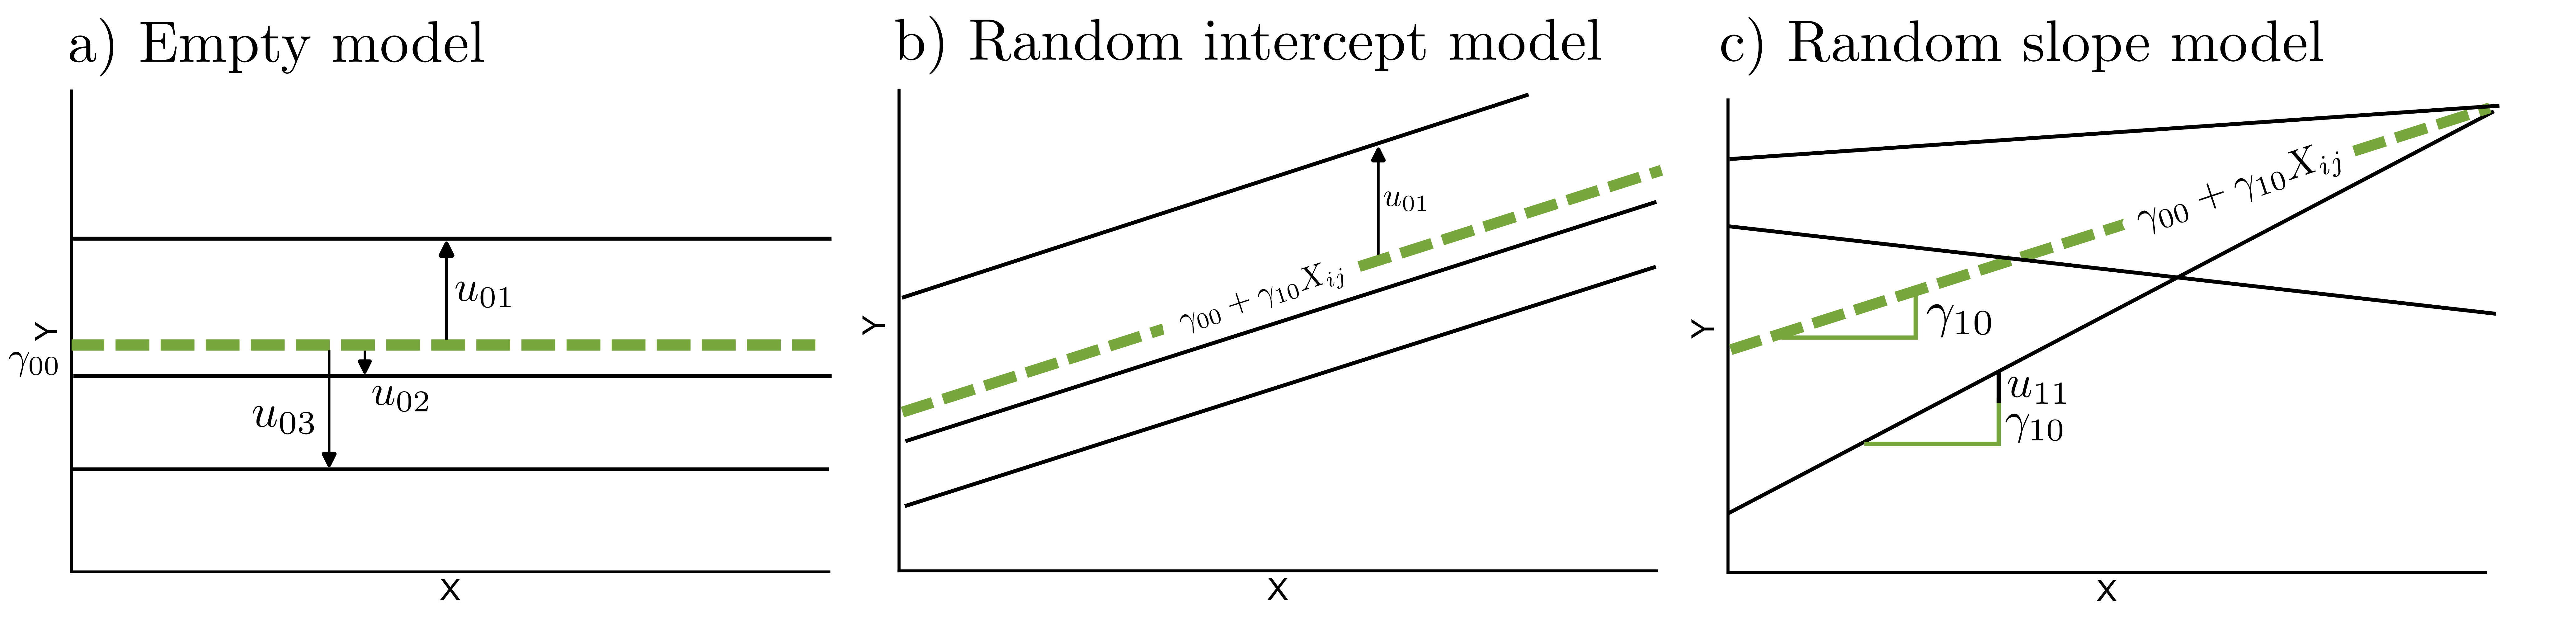
\includegraphics[keepaspectratio]{chapters/../figures/allmodels.png}}

}

\caption{\label{fig-mlmplots}Schematic illustration of common multilevel
model specifications in the level-1 coordinate space: empty model,
random intercept model, and random slope model. The green line
represents the fixed-effect prediction averaged across groups. The black
lines represent exemplary groups and their deviations from the fixed
effects. Individual-level observations are not displayed.}

\end{figure}%

\subsection{Level-1 and level-2 predictors in multilevel regression
models}\label{level-1-and-level-2-predictors-in-multilevel-regression-models}

Predictors can then be included to explain variability at level 1 and
level 2. At level 1, the outcome of a person \(i\) in group \(j\) is
modeled as a function of individual-level explanatory variables
\(X_{ij}\). For simplicity, the level-1 equation is given with a single
level-1 predictor: \begin{equation}\phantomsection\label{eq-mlm}{
Y_{ij} =  \beta_{0j} + \beta_{1j}X_{ij} + e_{ij}
}\end{equation} In this equation, \(\beta_{0j}\) is the intercept for
group \(j\), and \(\beta_{1j}\) is the corresponding slope in group
\(j\). In a random slope model, each group is allowed to have its own
intercept and slope. This model is illustrated on the right in
Figure~\ref{fig-mlmplots}. The variation between groups in these
coefficients is modeled at level 2, where \(\beta_{0j}\) and
\(\beta_{1j}\) can be decomposed into \emph{fixed effects}, representing
the average coefficients across groups (\(\gamma_{00}\) for the
intercept and \(\gamma_{10}\) for the slope), and group-specific
\emph{random effects}, representing deviations from these averages
(\(u_{0j}\) and \(u_{1j}\), respectively; Snijders \& Bosker
(\citeproc{ref-snijders}{2012}), p.~75). Without level-2 predictors, the
level-2 equations are: \[
\beta_{0j}
=
\underbrace{\gamma_{00}}_{\text{Fixed part}}
+
\underbrace{u_{0j}}_{\text{Random part}}
\] \[
\beta_{1j}
=
\underbrace{\gamma_{10}}_{\text{Fixed part}}
+
\underbrace{u_{1j}}_{\text{Random part}}
\] In order to explain between-group variability in the intercepts and
slopes, level-2 predictors \(Z_j\) may be included
(\citeproc{ref-snijders}{Snijders \& Bosker, 2012, p. 80}). Including
such predictors may reduce the unexplained variance of the random
effects \(u_{0j}\) and \(u_{1j}\). With a single level-2 predictor, the
model becomes:

\begin{equation}\phantomsection\label{eq-beta0j}{
\beta_{0j}
=
\gamma_{00} + \gamma_{01}Z_{j}
+
u_{0j}
}\end{equation}

\begin{equation}\phantomsection\label{eq-beta1j}{
\beta_{1j}
=
\gamma_{10} + \gamma_{11}Z_{j}
+
u_{1j}
}\end{equation} Here, the level-2 predictor \(Z_j\) is used to explain
systematic between-group differences in the level-1 intercepts and
slopes. The coefficient \(\gamma_{01}\) represents the expected
difference in the group-specific intercept \(\beta_{0j}\) associated
with a one-unit difference in \(Z_j\). Similarly, \(\gamma_{11}\)
represents the expected difference in the group-specific slope
\(\beta_{1j}\) associated with a one-unit difference in \(Z_j\). Thus,
\(\gamma_{11}\) describes a cross-level interaction: it indicates
whether the association between the individual-level predictor
\(X_{ij}\) and the outcome \(Y_{ij}\) differs depending on the
group-level variable \(Z_j\). The residual terms \(u_{0j}\) and
\(u_{1j}\) represent remaining between-group variation in intercepts and
slopes that is not explained by \(Z_j\). Substituting the level-2
equations Equation~\ref{eq-beta0j} and Equation~\ref{eq-beta1j} into the
level-1 equation Equation~\ref{eq-mlm} yields the combined multilevel
model:

\[
Y_{ij} =
\underbrace{\gamma_{00} + \gamma_{10}X_{ij} + \gamma_{01}Z_{j} + \gamma_{11}X_{ij}Z_{j}}_{\text{Fixed part}}
+
\underbrace{u_{0j} + u_{1j}X_{ij} + e_{ij}}_{\text{Random part}}
\]

In many empirical applications of multilevel models, the slope
\(\beta_{1j}\) is assumed to be constant across groups, so that no
random slope component is included (\(u_{1j} = 0\)). This leads to a
\emph{random-intercept model} (\citeproc{ref-snijders}{Snijders \&
Bosker, 2012, p. 45}). In its simpler form, the model also does not
include a cross-level interaction (\(\gamma_{11} = 0\)). \footnote{A
  cross-level interaction can technically be included in a
  random-intercept model. However, this assumes that slope differences
  are modeled only as a systematic function of the level-2 predictor,
  without allowing for remaining unexplained slope variation. For this
  reason, cross-level interactions are usually discussed together with
  random slopes; see Heisig \& Schaeffer (\citeproc{ref-heisig}{2019});
  Aguinis et al. (\citeproc{ref-aguinis}{2013}).}. This model allows for
baseline differences in the outcome between groups, whereas the strength
of the relationship between the level-1 predictor and the outcome is
assumed to be constant across groups. This model is illustrated in the
middle panel in Figure~\ref{fig-mlmplots}. The corresponding level-2
equations are: \[
\beta_{0j} = \gamma_{00} + \gamma_{01}Z_j + u_{0j}
\]

\[
\beta_{1j} = \gamma_{10}
\] The combined random-intercept equation therefore has only two random
components, the group-level random effect \(u_{0j}\) and the
individual-level residual \(e_{ij}\): \[ 
Y_{ij} = \gamma_{00} + \gamma_{10}X_{ij} + \gamma_{01}Z_j + u_{0j} + e_{ij}
\] \#\#\# Distributional assumptions of the multilevel regression model
Similar distributional assumptions are typically made for the level-2
random effects as for the residuals in single-level regression: they
have mean zero, constant variance across clusters, and are independent
of each other across clusters and independent of the level-1 residuals.
However, random effects within the same cluster - i.e.~the random
intercept \(u_{0j}\) and random slope \(u_{1j}\) - may be correlated and
are often expected to do so (\citeproc{ref-snijders}{Snijders \& Bosker,
2012, p. 76}). Additionally, random effects are commonly assumed to
follow a normal distribution for convenience, as it facilitates the
likelihood-based estimation of the unknown parameters
(\citeproc{ref-fahrmeir}{Fahrmeir et al., 2021, p. 388}). For a model
with both a random intercept and a random slope, these assumptions can
be summarized by a bivariate normal distribution, \[
\begin{aligned}
\begin{pmatrix}
u_{0j} \\
u_{1j}
\end{pmatrix}
&\sim \mathcal{N}
\left(
\begin{pmatrix}
0 \\
0
\end{pmatrix},
\mathbf{T}
\right),
\qquad
\mathbf{T} =
\begin{pmatrix}
\tau_0^2 & \tau_{01} \\
\tau_{01} & \tau_1^2
\end{pmatrix}
\end{aligned},
\] where \(\tau_0^2\) denotes the variance of the random intercepts
across groups, and \(\tau_1^2\) denotes the variance of the random
slopes across groups. The covariance \(\tau_{01}\) captures the
association between random intercepts and random slopes within the same
group. For example, a positive covariance would indicate that groups
with higher-than-average intercepts also tend to have
steeper-than-average slopes.

The level-1 residuals are typically assumed to be normally distributed
with mean zero and constant variance (\(\sigma^2\)):

\[
e_{ij} \sim \mathcal{N}(0,\sigma^2)
\] Furthermore they are assumed to be independent of the level-2 random
effects:

\[
\text{Cov}(u_{0j}, e_{ij}) = 0, \qquad
\text{Cov}(u_{1j}, e_{ij}) = 0.
\]

\subsection{Contextual effects in multilevel
models}\label{contextual-effects-in-multilevel-models}

As mentioned previously, individuals nested within the same group share
a common context. In some cases, variables measured at the individual
level may therefore be relevant in two different ways. First, they may
describe how individuals differ from other individuals within the same
group. Second, when aggregated to the group level, they may describe
characteristics of the group context itself. Consider again the ensemble
example, where students' practice duration was used to explain the
musical self concept of students. A student who practices more than
their peers may feel more competent and report a higher musical
self-concept. But at the same time, students often compare their own
practice behavior with that of other ensemble members; and students in
ensembles where everyone practices a lot may feel less competent,
because upward social comparisons become more likely. This leads to two
possible hypotheses:

\begin{enumerate}
\def\labelenumi{\arabic{enumi}.}
\tightlist
\item
  Students who practice more than others in their ensemble tend to
  report a higher musical self-concept.
\item
  Students in ensembles with a higher average practice time may report a
  lower musical self-concept.\\
  This example illustrates why it can be important to distinguish
  within-group and between-group associations. The within-group
  association describes how individual deviations from the group mean
  are related to the outcome. The between-group association describes
  how differences between group means are related to the outcome. A
  contextual effect is present when the group-level aggregate is
  associated with the outcome after controlling for individual
  differences within groups (\citeproc{ref-raudenbush}{Raudenbush \&
  Bryk, 2010, p. 139}). A random-intercept model provides a convenient
  framework for such analyses. To disentangle these processes, group
  means of a level-1 predictor may be included in the model as
  additional level-2 predictors. To separate within- and between-group
  effects, the level-1 predictor is commonly group-mean-centered:
  Instead of using \(X_{ij}\) directly, the centered predictor
  \((X_{ij} - \bar{X}_j)\) is entered into the model
  (\citeproc{ref-snijders}{Snijders \& Bosker, 2012, p. 58}). A random
  intercept model including such a decomposition can be written like
  this\footnote{The group mean \(\bar{X}_{j}\) is treated as an observed
    (manifest) aggregate in this approach. Group means can also be
    modeled as latent variables, thereby accounting for measurement
    error and sampling variability (\citeproc{ref-luedtkecontext}{Lüdtke
    et al., 2008}).}: \begin{equation}\phantomsection\label{eq-RI}{ 
  Y_{ij} = \gamma_{00} + \gamma_{10}(X_{ij} - \bar{X}_{j}) + \gamma_{01}\bar{X}_{j} + u_{0j} + e_{ij}
  }\end{equation} In this model, the effect of weekly practice duration
  on \(Y_{ij}\), the musical self-concept of student \(i\) in ensemble
  \(j\), is separated into the \emph{within-group effect}
  \(\gamma_{10}\), indicating how a student's own practice time relates
  to their musical self-concept while controlling for the ensemble
  context, and the \emph{between-group effect} \(\gamma_{01}\),
  indicating how the ensemble's average practice time relates to
  students' musical self-concept, controlling for individual deviations
  from the group mean. The difference between these two coefficients,
  \(\gamma_{01}\)-\(\gamma_{10}\), represents the \emph{contextual
  effect} (\citeproc{ref-raudenbush}{Raudenbush \& Bryk, 2010, p. 139}).
  For the remainder of this thesis, the focus lies on this particular
  random intercept model.
\end{enumerate}

\subsection{The intraclass correlation coefficient
(ICC)}\label{the-intraclass-correlation-coefficient-icc}

In the random intercept model, the variance components are given by \[
u_{0j} \sim \mathcal{N}(0,\tau_0^2),
\qquad
e_{ij} \sim \mathcal{N}(0,\sigma^2),
\qquad
\text{Cov}(e_{ij}, u_{0j}) = 0 .
\] From these variance components, the proportion of variability that is
attributable to between-group differences can be calculated. This
quantity is referred to as the \emph{intraclass correlation coefficient}
(ICC). In the empty model, the ICC is equal to the correlation between
the outcomes of two randomly chosen individuals from the same group
(\citeproc{ref-snijders}{Snijders \& Bosker, 2012, p. 18}). In models
including predictors, the ICC is interpreted conditionally on the
predictors, that is, as the correlation between two individuals from the
same group who share identical predictor values (also referred to as the
\emph{residual ICC}) (\citeproc{ref-snijders}{Snijders \& Bosker, 2012,
p. 52}). Formally, the ICC in a random intercept model is defined as \[
ICC = \frac{\tau_0^2}{\tau_0^2 + \sigma^2}
\] The ICC is an important diagnostic metric because it indicates the
extent to which residual variance in \(Y_{ij}\) is attributable to
differences between groups. If ICC = 0, no residual between-group
variance is estimated in the model. Larger ICC values, in contrast,
indicate increasing similarity of observations within groups and hence
stronger statistical dependency. Ignoring this dependency and applying a
classical linear model can lead to biased standard errors, confidence
intervals, and hypothesis tests (\citeproc{ref-aarts}{Aarts et al.,
2014}; \citeproc{ref-fahrmeir}{Fahrmeir et al., 2021, p. 370}).

\subsection{Estimation of parameters in multilevel
models}\label{sec-est}

The random intercept model is defined by the fixed effects \(\gamma\)
and the variance components of the random effects, \(\sigma^2\) and
\(\tau_0^2\) (\citeproc{ref-snijders}{Snijders \& Bosker, 2012, p. 60}).
In practice, however, these model parameters are unknown and must be
estimated from the observed data. In many applications, including the
contextual-effect setting considered in this thesis, substantive
hypotheses primarily concern fixed effects. In the ensemble example
introduced above, for instance, the within- and between-group
associations between practice time and musical self-concept would be
represented by fixed-effect parameters. The variance components are
nevertheless essential, because they influence the estimated uncertainty
of the fixed-effect estimates. Based on the resulting parameter
estimates, their estimated uncertainty, and assumptions about the
sampling distribution of the estimators, inferences about the
corresponding population parameters are drawn
(\citeproc{ref-raudenbush}{Raudenbush \& Bryk, 2010, p. 57f}.). The
steps of this process are illustrated in more detail in
Figure~\ref{fig-est}. Aspects of the observed data may pose challenges
to the reliable performance of this `inferential machinery'. Two central
challenging aspects, namely small sample sizes and missing data, will be
discussed in the following chapters.

\begin{figure}

\centering{

\pandocbounded{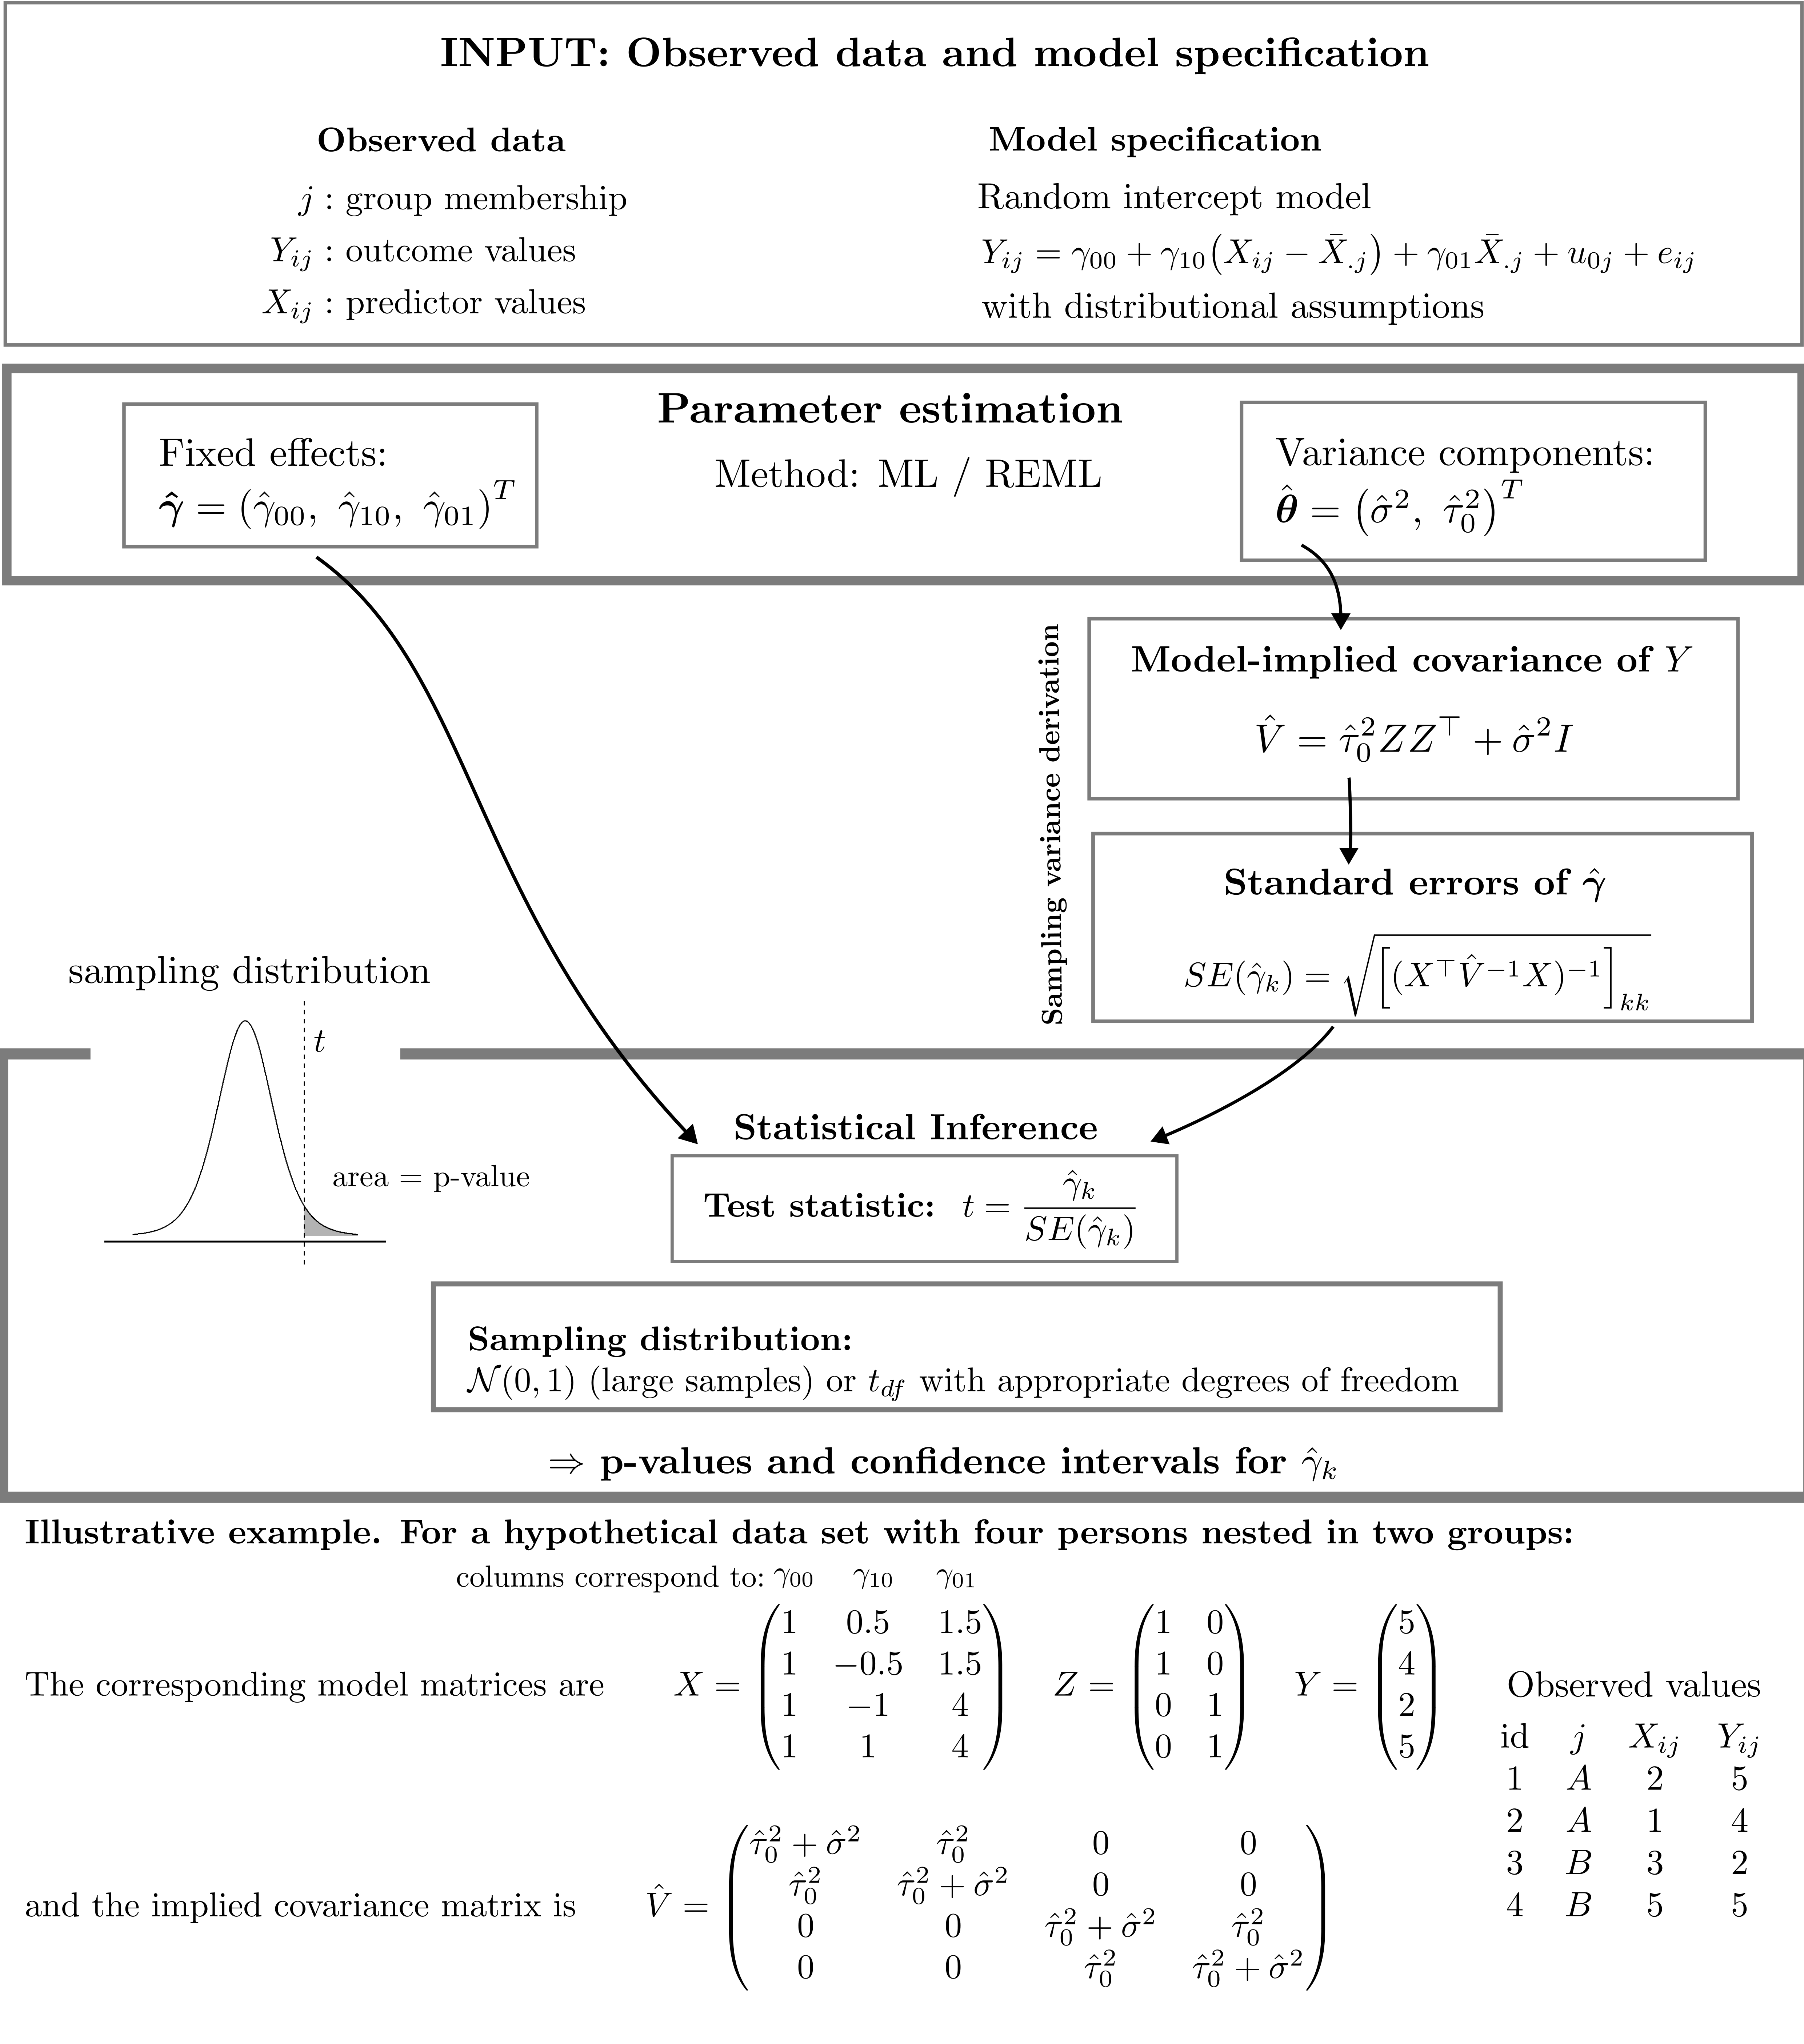
\includegraphics[keepaspectratio]{figures/estimation.png}}

}

\caption[Frequentist inferential process in a random intercept
model]{\label{fig-est}Schematic representation of the frequentist
inferential process in a random intercept model, based on Snijders \&
Bosker (\citeproc{ref-snijders}{2012}) and Raudenbush \& Bryk
(\citeproc{ref-raudenbush}{2010}). \small In the first step, fixed
effects and variance components are estimated from the observed data,
commonly using maximum likelihood (ML) or restricted maximum likelihood
(REML) estimation. The estimated random-intercept variance
\(\hat{\tau}_0^2\) and residual variance \(\hat{\sigma}^2\), together
with the random-effects design matrix \(Z\), determine the estimated
variance-covariance matrix of the outcome vector, \(\hat V\). In the
random-intercept model, \(Z\) encodes group membership and thereby
represents that observations from the same group share the same random
intercept. The estimated uncertainty of the fixed-effect estimates is
then derived from \(\hat V\) and the fixed-effects design matrix \(X\).
This matrix contains one row for each observation and columns for the
fixed-effect terms in the model. For a given fixed effect
\(\hat{\gamma}_k\), the corresponding standard error quantifies the
estimated sampling variability of the estimator. The point estimate and
its standard error are used to form a test statistic, which is evaluated
against an assumed sampling distribution to obtain \(p\)-values and
confidence intervals. Thus, frequentist inference for fixed effects
depends not only on the point estimates themselves, but also on the
estimated variance components and on assumptions about the sampling
distribution of the estimators. \normalsize}

\end{figure}%

\section{Small sample sizes in multilevel models}\label{sec-small}

Frequentist estimation procedures for linear multilevel models typically
rely on large-sample (asymptotic) theory. In multilevel models, the
number of groups is particularly important. Consider again the musical
self-concept study with 150 students nested in 15 ensembles. Although
150 participants may seem like a reasonably large sample, the number of
ensembles is still small. Information about between-ensemble variation
and level-2 effects is therefore based on only 15 higher-level units.
Simulation studies suggest that approximately 25--30 clusters are often
required for reliable estimation, depending on the model specification
and the parameters of interest (\citeproc{ref-maashox}{Maas \& Hox,
2005}; \citeproc{ref-mcneish17}{McNeish, 2017a};
\citeproc{ref-mcneishstaple14}{McNeish \& Stapleton, 2016b}), but this
is often difficult to achieve because recruiting a large number of
groups can be challenging and costly. When the number of groups is
small, several components of the inferential procedure may perform
poorly if no corrections are used, particularly the estimation of
level-2 variance components, the calculation of standard errors, and the
approximation of degrees of freedom for fixed-effect tests
(\citeproc{ref-elff}{Elff et al., 2021}; \citeproc{ref-maashox}{Maas \&
Hox, 2005}; \citeproc{ref-mcneishcoll}{McNeish, 2017b}).

\textbf{Estimation of coefficients and variance components.} For
correctly specified linear multilevel models, ML estimates of fixed
effect coefficients are unbiased under quite general conditions
(\citeproc{ref-elff}{Elff et al., 2021}, Appendix A.3;
\citeproc{ref-kackar}{Kackar \& Harville, 1981}). Importantly, this
unbiasedness result does not depend on the level-1 or level-2 sample
size and a small number of groups therefore does not in itself imply
biased fixed-effect point estimates. The estimation of variance
components, however, is more delicate. In ML estimation, fixed effects
and variance components are estimated from the same likelihood,
typically via iterative procedures like the Expectation Maximization
(EM) algorithm (\citeproc{ref-raudenbush}{Raudenbush \& Bryk, 2010, p.
52}). This leads to systematic underestimation of variance components in
small samples, because the uncertainty about the fixed effects is not
accounted for (\citeproc{ref-raudenbush}{Raudenbush \& Bryk, 2010, p.
53}). REML addresses this issue by separating the estimation
conceptually, which leads to less downward-biased variance component
estimates, while ML and REML become asymptotically equivalent as sample
size increases (\citeproc{ref-mcneishcoll}{McNeish, 2017b}).
Nevertheless, even under REML, the estimated variance of the
fixed-effect estimators may still be too small in small samples for two
reasons. First, the variance formula treats the estimated variance
components \(\hat{\theta}\) as known and therefore ignores their
sampling variability (\citeproc{ref-kackarcorr}{Kackar \& Harville,
1984}). Second, the REML variance expression itself relies on asymptotic
approximations (\citeproc{ref-mcneishcoll}{McNeish, 2017b}). Both issues
can lead to underestimated standard errors. Several small-sample
corrections have been proposed to address this additional problems,
among which the Kenward--Roger procedure is one of the most widely used
(\citeproc{ref-mcneishcoll}{McNeish, 2017b}).

\textbf{Choice of degrees of freedom.} REML estimation and small-sample
adjustments such as Kenward--Roger can reduce some of the inferential
problems described above. However, inference also requires choosing an
appropriate reference distribution for test statistics and confidence
intervals. In small samples, a \(t\)-distribution is typically
recommended instead of a standard normal distribution
(\citeproc{ref-snijders}{Snijders \& Bosker, 2012, p. 95}). Its shape is
determined by the degrees of freedom, which can be understood as the
amount of independent information remaining after accounting for
estimated parameters (\citeproc{ref-pandey}{Pandey \& Bright, 2008}). In
multilevel models, degrees of freedom generally cannot be calculated
exactly and must therefore be approximated
(\citeproc{ref-snijders}{Snijders \& Bosker, 2012, p. 95}). Different
approximations are available. For example, the Kenward--Roger procedure
includes a small-sample approximation of the degrees of freedom based on
the Satterthwaite method (\citeproc{ref-mcneishcoll}{McNeish, 2017b}). A
simpler approximation, described by Raudenbush \& Bryk
(\citeproc{ref-raudenbush}{2010, p. 58}), Snijders \& Bosker
(\citeproc{ref-snijders}{2012, p. 95}), and Elff et al.
(\citeproc{ref-elff}{2021}), follows the general idea of degrees of
freedom as information minus estimated parameters. For level-1
coefficients, the degrees of freedom are approximated by the total
number of level-1 observations minus the number of level-1 predictors
and the intercept. For level-2 coefficients, the degrees of freedom are
approximated by the number of level-2 units minus the number of level-2
predictors and the intercept:
\begin{equation}\phantomsection\label{eq-df}{
df_{Lv1} = N_1 - r - 1, \qquad df_{Lv2} = N_2 - q - 1
}\end{equation} where \(N_1\) is the total number of level-1
observations, \(N_2\) is the number of level-2 units, \(r\) is the total
number of predictors, and \(q\) is the number of level-2 predictors.

\textbf{Bayesian estimation as an alternative.} As an alternative to the
frequentist framework predominantly presented here, Bayesian estimation
is often recommended for small samples (\citeproc{ref-depaoli}{Depaoli
\& Clifton, 2015}; \citeproc{ref-kadane}{Kadane, 2015};
\citeproc{ref-mcneishbay}{McNeish, 2016a};
\citeproc{ref-vandeschoot}{Van De Schoot et al., 2014}). Unlike
frequentist inference based on asymptotic sampling distributions,
Bayesian inference represents uncertainty through posterior
distributions and therefore does not rely on small-sample corrections
for standard errors or degrees of freedom
(\citeproc{ref-mcneishbay}{McNeish, 2016a}). The incorporation of prior
information about parameters may further improve estimation accuracy
when the data provide limited information
(\citeproc{ref-gelmanbook}{Gelman et al., 2025, p. 355};
\citeproc{ref-smid}{Smid et al., 2020}). Bayesian estimation will be
revisited below in the context of missing data.

\section{Missing data in multilevel
models}\label{missing-data-in-multilevel-models}

In the study about musical self-concept, you could find after data
collection that some students in several ensembles did not report how
many hours they practice per week. They completed the questionnaire on
musical self-concept but left the practice question blank. The reason
for this is unknown: they might have forgotten to answer the question,
skipped it intentionally, or misunderstood it. Regardless of the reason,
the data set now contains missing values. How should these missing
observations be handled in the analysis?

Missing data (i.e., incomplete data sets) are a widespread issue in
empirical research and of course also apply to multilevel data, for
example, because individuals drop out of studies or forget to fill out
certain items of a questionnaire. Three major concerns commonly arise
from data that contain missing values (\citeproc{ref-luedtke}{Lüdtke et
al., 2007}):

\begin{enumerate}
\def\labelenumi{\arabic{enumi}.}
\tightlist
\item
  The effective sample size is reduced, leading to lower efficiency in
  estimation (this is especially troublesome if the would-be sample size
  is already small)
\item
  Typical statistical methods are difficult to conduct, because they
  were designed for complete data.
\item
  Parameter estimation may be biased, if the missing and the observed
  data differ from each other systematically
\end{enumerate}

Therefore, it is crucial to treat missing data appropriately. In the
last three decades, this issue has received attention in psychological
research, and modern methods were developed
(\citeproc{ref-endersbook}{Enders, 2022}; \citeproc{ref-SG2002}{Schafer
\& Graham, 2002}), more recently also for the more complex case of
multilevel data (\citeproc{ref-endersupdate}{Enders, 2025};
\citeproc{ref-luedtkeMI}{Lüdtke et al., 2017}). This chapter discusses
these methods, after giving a short introduction into different missing
data mechanisms and patterns.

\subsection{Missing data mechanisms}\label{missing-data-mechanisms}

Why data are missing can have multiple reasons, and different mechanisms
may lead to different consequences in statistical inference. Rubin and
Little (\citeproc{ref-littlerubin87}{1987};
\citeproc{ref-rubin76}{Rubin, 1976}) introduced a typology and
theoretical framework of missing data mechanisms that describes the
relationship between the observed and the missing data. These mechanisms
also apply to multilevel data, while the situation becomes even more
complex because missing values can occur in the outcome, in level-1
predictors, in level-2 predictors, or even in the grouping variable (or
combinations of these, \citeproc{ref-buuren}{Van Buuren, 2018}). The
missing data mechanism is generally not empirically testable from the
observed data alone and assumptions about the mechanism must therefore
be theoretically justified (\citeproc{ref-endersbook}{Enders, 2022, pp.
14--17}).

\textbf{Missing completely at random (MCAR)}. The hypothetical complete
data matrix \(Y_{com}\) can be partitioned into observed, \(Y_{obs}\),
and missing parts, \(Y_{mis}\). \(R\) denotes the
missingness\footnote{\(R\) is treated as a set of random variables that
  indicate for each value if it is missing or not
  (\citeproc{ref-SG2002}{Schafer \& Graham, 2002}).}. Missing values are
considered to be MCAR if the distribution of missingness is independent
of both the observed and the unobserved data
(\citeproc{ref-SG2002}{Schafer \& Graham, 2002}): \[
P(R \mid Y_{com}) = P (R)
\] In other words, no variable (observed or unobserved) is predictive of
missingness and every individual has the same chance of missing values
(\citeproc{ref-endersbook}{Enders, 2022, p. 6}).

\textbf{Missing at random (MAR)}. The MAR mechanism describes the case
when the probability of missingness may depend on observed data, but not
on the unobserved values themselves once the observed data are taken
into account (\citeproc{ref-endersbook}{Enders, 2022, p. 8}): \[
P(R \mid Y_{com}) = P (R \mid Y_{obs})
\] Missingness is therefore not random, as the name would suggest, but
\emph{conditionally random}: After controlling for the observed data,
the missingness is purely random (\citeproc{ref-endersbook}{Enders,
2022, p. 8}). For example, younger students may be more likely to skip
the question on weekly practice duration, for instance due to reduced
concentration toward the end of the questionnaire. If age is fully
observed and included in the missing-data procedure, the MAR mechanism
may be plausible.

\textbf{Missing not at random (MNAR)}. If missingness depends on
unobserved values, this is called a missing not at random process: \[
P(R \mid Y_{com}) = P (R \mid Y_{obs}, Y_{mis})
\] Two individuals with identical scores in all observed variables
therefore no longer have the same chance of missing values, because this
chance depends on the unavailable, missing information itself
(\citeproc{ref-endersbook}{Enders, 2022, p. 11}). For example, students
who practice less may be more likely to skip the question on weekly
practice duration. If no observed variables can account for this
behavior, missingness depends on the practice duration itself, which
represents a MNAR mechanism.

The approaches mentioned in this thesis generally rely on the assumption
that data are MAR. Methods for dealing with MNAR processes are not
discussed in this thesis.

\subsection{Methods for handling missing
data}\label{methods-for-handling-missing-data}

Many estimation procedures require complete data. Therefore, missing
data must be handled explicitly before model estimation. If researchers
do not actively specify a method, statistical software often defaults to
using only complete observations (\citeproc{ref-luedtke}{Lüdtke et al.,
2007}). This simple ad hoc procedure is called \emph{listwise deletion}
(LD) or \emph{complete case analysis}. Cases with at least one missing
value are discarded, and the model is estimated using only complete
observations (\citeproc{ref-graham09}{Graham, 2009}). In multilevel
settings, missingness on the group level implies that all individuals in
this group are excluded as well.

LD is generally not recommended, because parameter estimates can be
substantially biased when missingness is not MCAR. In addition, partial
data is unused, which reduces statistical power
(\citeproc{ref-endersbook}{Enders, 2022, p. 24}). More modern and
better-performing methods are available and will be introduced in the
following sections. These approaches can be broadly divided into two
classes:\\
1. \emph{Model-based approaches} to missing data base parameter
estimation and inference directly on the incomplete data, for example
via the observed-data likelihood or the posterior distribution
(\citeproc{ref-little20}{Little \& Rubin, 2020, p. 25}). 2.
\emph{Imputation-based approaches} first replace missing values by one
or more plausible values, creating one or more completed data sets that
can then be analyzed using standard complete-data methods.

\subsubsection{Multiple Imputation}\label{multiple-imputation}

Multiple imputation (MI) is an imputation-based method, as the name
suggests. The basic idea is to replace missing values with plausible
draws (``imputations'') from their predictive distribution. The
substantive analysis model is then fitted to the imputed data. In order
to include the uncertainty due to missing values, in MI several
imputations for each missing observation are generated. By incorporating
the variance between these imputations, the additional uncertainty can
be captured (\citeproc{ref-endersbook}{Enders, 2022, p. 283}). The
analysis of incomplete data is separated into three steps: imputation,
analysis, and pooling.

\textbf{Creating imputations.} Imputations can be understood as
``predicted values plus noise'' (\citeproc{ref-endersbook}{Enders, 2022,
p. 266}). That is, missing values are replaced by plausible values drawn
from an imputation model, so that the resulting completed data sets
reflect both the predicted value and uncertainty around this prediction
(\citeproc{ref-murray}{Murray, 2018}). A finite number, usually between
\(m\) = 20 and \(m = 100\) (\citeproc{ref-graham07}{Graham et al.,
2007}) of imputations is saved, leading to \(m\) completed data sets.
The imputation model can either be specified jointly for all variables
(\emph{joint imputation}) or individually (\emph{fully conditional
specification}). Both approaches can be extended to multilevel data
structures (\citeproc{ref-enders16}{Enders et al., 2016}), but in this
thesis, only joint imputation is considered. In this approach, a single
multivariate distribution for all variables with missing values is
specified, often the multivariate normal distribution for continuous
variables (\citeproc{ref-endersbook}{Enders, 2022, p. 263}).

\textbf{Specifying the imputation model.} A crucial point in the choice
of a valid imputation model is compatibility with the focal analysis
model that is used later on. That is, the imputation model must reflect
the key structural features of this analysis model
(\citeproc{ref-grundMI18}{Grund et al., 2018b};
\citeproc{ref-meng}{Meng, 1994}). At the same time, the imputation model
is allowed to be richer than the analysis model. Including additional
effects or variables that are not part of the analysis model as
\emph{auxiliary variables}\footnote{Auxiliary variables are variables
  whose only purpose is to improve the missing-data imputation
  (\citeproc{ref-collins}{Collins et al., 2001}).} is considered
beneficial for parameter estimation (\citeproc{ref-collins}{Collins et
al., 2001}; \citeproc{ref-schafer03}{Schafer, 2003}). These variables
may either be causes of missingness, thereby making the missing at
random (MAR) assumption more plausible, or they may correlate with
variables that contain missing values, which can increase the precision
of the imputations and reduce bias in parameter estimates
(\citeproc{ref-collins}{Collins et al., 2001}).

For a random-intercept analysis model, the \emph{multivariate empty
model} generally represents a suitable joint imputation model. In this
approach, all level-1 and level-2 variables included in the imputation
model are treated as outcomes, and their variances and covariances are
decomposed into between- and within-group components without specifying
predictors (\citeproc{ref-grundMI16}{Grund et al., 2016b}). In this way,
the multilevel structure of the data and the associations among
variables at the respective levels are preserved. This also provides the
relevant within- and between-group information for a random-intercept
model with a contextual effect. For the model introduced in
Equation~\ref{eq-RI}, an appropriate joint imputation model with one
additional level-2 variable can be written as:

\begin{equation}\phantomsection\label{eq-imputationmodel}{ 
\left(
\begin{matrix}
Y_{ij} \\
X_{ij} \\
W_j
\end{matrix}
\right)
=
\left(
\begin{matrix}
\beta_{0Y} \\
\beta_{0X} \\
\beta_{0W}
\end{matrix}
\right)
+
\left(
\begin{matrix}
u_{Yj} \\
u_{Xj} \\
u_{Wj}
\end{matrix}
\right)
+
\left(
\begin{matrix}
e_{Yij} \\
e_{Xij} \\
0
\end{matrix}
\right)
}\end{equation}

\(W_j\) represents a level-2 variable and therefore has no level-1
residual term. If \(W_j\) is not included in the analysis model, it can
serve as an auxiliary variable. For example, in the musical self-concept
study, the years of teaching experience of the ensemble teachers might
be available. Although this variable is not part of the subsequent
analysis model, it may correlate with practice behavior or musical
self-concept and could therefore serve as an auxiliary level-2 variable.
The random effects and residuals are assumed to follow multivariate
normal distributions: \[
\left(
\begin{matrix}
u_{Yj} \\
u_{Xj} \\
u_{Wj}
\end{matrix}
\right)
\sim N(0,\Psi),
\qquad
\left(
\begin{matrix}
e_{Yij} \\
e_{Xij}
\end{matrix}
\right)
\sim N(0,\Sigma)
\] where the covariance matrix \(\Psi\) captures the between-group
variability and covariation of the random intercepts and \(\Sigma\)
represents the within-group covariance structure of the level-1
residuals:

\[
\Psi =
\left[
\begin{matrix}
\psi_y^2 & \psi_{yx} & \psi_{yw} \\
\psi_{yx} & \psi_x^2 & \psi_{xw} \\
\psi_{yw} & \psi_{xw} & \psi_w^2
\end{matrix}
\right],
\qquad
\Sigma =
\left[
\begin{matrix}
\sigma_y^2 & \sigma_{yx} \\
\sigma_{yx} & \sigma_x^2
\end{matrix}
\right].
\] \textbf{Analyzing the completed data sets and pooling the results.}
After the imputation step, researchers are in the comfortable position
to have \emph{m} completed data sets that can be analyzed using standard
frequentist methods. To each of the data sets, the substantive analysis
model of interest (e.g., the random intercept model) is now fitted. Each
analysis proceeds according to the standard estimation procedure
described in Section~\ref{sec-est}, up to the computation of parameter
estimates and their standard errors. Hypothesis testing is not conducted
at this stage. The result of this step is a set of \emph{m} parameter
estimates and corresponding standard errors. These \emph{m} estimates
and standard errors are aggregated into a single set of results
following Rubin's pooling rules (\citeproc{ref-rubinbook87}{Rubin,
1987}). He defined the point estimates of effects as the arithmetic
average of the \(m\) estimates:

\[
\hat{\theta} = \frac{1}{m}
\sum_{k=1}^{m}
\hat{\theta}_k
\] \(\hat{\theta}\) is the pooled point estimate, and \(\hat{\theta}_k\)
is the estimate from data set \(k\) (\(k=1, ...,m\)).

For the pooled standard errors, both the within-imputation variance
(which is based on a complete data set) and the between-imputation
variance (which adds the uncertainty due to missing values) are
combined. The within-imputation variance is the arithmetic average of
the imputation's variances (standard errors squared):

\[
\bar{V}_w
=
\frac{1}{m}
\sum_{k=1}^{m}
SE^2_k
\] The between-imputation variance is defined as the variance of point
estimates between imputations that is due to uncertainty caused by the
missing values:

\[
V_b
=
\frac{1}{m-1}
\sum_{k=1}^{m}
(\hat{\theta}_k - \hat{\theta})^2
\] The total pooled standard error combines the within-imputation
variance \(\bar{V}_w\) and the between-imputation variance \(V_b\): \[
SE
=
\sqrt{
\bar{V}_w
+ V_b
+ \frac{V_b}{m}}
\] The third term in this expression acts as a correction factor for
using a finite number of imputations (\citeproc{ref-endersbook}{Enders,
2022, p. 284}). As the number of imputations \(m\) increases, this
correction term approaches zero. With an appropriate point estimate and
standard error, the remaining step (see Figure~\ref{fig-est}) is the
choice of the sampling distribution. Rubin proposed a calculation method
for degrees of freedom of the t-distribution, that is based on the
relative increase of variance due to missing values RIV
(\(RIV = \frac{(1 + 1/m)V_b}{\bar{V}_w}\)) and the number of imputations
\(m\): \[
df_R
=
(m-1)
\left(
1+\frac{1}{RIV^2}
\right)
\] This formula assumes that the degrees of freedom of the complete data
are effectively infinite (\citeproc{ref-barnard}{Barnard \& Rubin,
1999}). In smaller samples, the classic Rubin formula therefore tends to
produce degrees of freedom that are too large, sometimes even larger
than the degrees of freedom of the complete data. Barnard and Rubin
(\citeproc{ref-barnard}{1999}) thus proposed a small-sample-adjusted
degrees-of-freedom calculation for pooled parameters. Their formula
downweights the complete-data degrees of freedom to account for the
uncertainty due to missing values. As the complete-data degrees of
freedom cannot easily be obtained for multilevel analyses, a suitable
degrees-of-freedom approximation must be chosen for the analysis.
Possible approaches include the methods described in
Section~\ref{sec-small}, but a specific recommendation for multilevel
models does not exist.

\subsubsection{Full Information Maximum Likelihood
(FIML)}\label{full-information-maximum-likelihood-fiml}

Full information maximum likelihood (FIML) is a model-based approach in
which parameter estimates are obtained directly by maximizing the
likelihood of the observed data (\citeproc{ref-endersbook}{Enders, 2022,
p. 98}). Under the assumption that data are missing at random (MAR),
FIML yields unbiased and efficient parameter estimates
(\citeproc{ref-mcneish17}{McNeish, 2017a}). Incorporating auxiliary
variables is less straightforward in FIML than in multiple imputation.
Nevertheless, several approaches have been proposed to include auxiliary
information in FIML estimation, such as the saturated correlates model
or the extra dependent variable approach
(\citeproc{ref-grahamFIML}{Graham, 2003}), as well as the factored
regression framework described below for the Bayesian missing-data
approaches.\\
For the random intercept model with group-mean effects considered in
this thesis, FIML is not always well suited when missingness occurs in
predictor variables. In such cases, maximum likelihood estimation
requires additional distributional assumptions about the distribution of
the predictors in order to incorporate them into the likelihood function
(\citeproc{ref-grundMI18}{Grund et al., 2018b}). In multilevel models
with manifest group means, these assumptions may lead to biased
estimates of between-group effects (\citeproc{ref-grundapa}{Grund et
al., 2019}).

\subsubsection{Fully Bayesian
Estimation}\label{fully-bayesian-estimation}

A Bayesian framework can naturally be applied to missing-data problems.
In contrast to the two-step procedure of multiple imputation, Bayesian
missing-data analysis directly uses the posterior distribution of the
model parameters conditional on the observed data for statistical
inference. Missing values are treated as additional unknown quantities.
To simulate these values during estimation, a model for the variables
with missing data must be specified. A convenient way to specify the
joint distribution of the outcome and the variables with missing values
is to apply the probability chain rule and express the joint
distribution as a product of conditional distributions, which is
referred to as \emph{sequential specification} or \emph{factored
regression specification} (\citeproc{ref-luedtke20}{Lüdtke et al.,
2020}):

\[ 
g\left(y,\ x;\gamma\right)=g_y\left(y \middle| x;\gamma_y\right) \times g_x(x;\gamma_x)
\] where \(\gamma = (\gamma_y, \gamma_x)\) denotes the vector of all
model parameters. Here, the joint density is decomposed into two
components. The first term \(g_y(y \mid x; \gamma_y)\) corresponds to
the density implied by the analysis model, describing the conditional
distribution of the outcome given the covariate \(X\). The second term
\(g_x(x; \gamma_x)\) specifies a model for the distribution of the
covariate \(X\). Each conditional distribution in a sequential modeling
framework is typically specified as a regression model. Consequently,
the implied joint distribution is constructed from a sequence of
conditional models, each imposing its own distributional assumptions.

An advantage of this formulation is its flexibility: it allows the
inclusion of variables with different measurement scales and facilitates
the use of auxiliary variables that are not part of the substantive
analysis model (\citeproc{ref-daniels}{Daniels et al., 2014};
\citeproc{ref-erler}{Erler et al., 2016}). For example, auxiliary
variables such as \(W_j\) may be included to improve the imputation of
missing values while the substantive model of interest is still
estimated without \(W_j\). For this purpose, auxiliary variables can be
placed in the first position of the factored regression, so that the
analysis variables predict the auxiliary variables
(\citeproc{ref-endersbook}{Enders, 2022, p. 215}):

\begin{equation}\phantomsection\label{eq-frs}{ 
g\left(y,\ x,w;\gamma\right)=g_w\left(w\middle| y,x;\gamma_w\right) \times g_y\left(y\middle| x;\gamma_y\right) \times g_x(x;\gamma_x)
}\end{equation} Because all missing values are resampled in each
iteration, the uncertainty due to missing data is automatically included
in the posterior distribution (\citeproc{ref-erler}{Erler et al.,
2016}).

\subsection{Present study}\label{present-study}

Both challenges considered here --- small sample sizes and missing data
--- often co-occur in empirical research, but missing-data methods have
rarely been investigated in small-sample settings. For multiple
imputation, some studies suggest that small-sample adjustments applied
during pooling may improve inferential performance in both single-level
and multilevel contexts (\citeproc{ref-mcneish17}{McNeish, 2017a},
\citeproc{ref-mcneishgrowth}{2018}). However, these adjustments have not
been compared to standard inferential approaches based on unadjusted
degrees of freedom, and the models considered did not incorporate
contextual predictors. Fully Bayesian estimation may offer a promising
model-based alternative to MI, as it naturally accommodates both missing
predictor values and small sample sizes. It is often recommended in more
complex multilevel models, for example in the presence of nonlinearities
or interaction effects (\citeproc{ref-depaoli}{Depaoli \& Clifton,
2015}; \citeproc{ref-endersmodel}{Enders et al., 2020};
\citeproc{ref-muthen12}{Muthén \& Asparouhov, 2012}). However, it may
also represent a suitable alternative to likelihood-based approaches
such as FIML in simpler models with contextual effects, where the
handling of missing predictor variables and the construction of group
means may lead to biased estimates (\citeproc{ref-grundapa}{Grund et
al., 2019}). To evaluate this, the present study uses a simulation
design to compare methods for handling missing data in a predictor
variable in a small-sample multilevel random intercept model. In
particular, it examines whether applying a small-sample-adjusted
degrees-of-freedom approximation with the \(N_2 - q - 1\) heuristic
(Equation~\ref{eq-df}) after multiple imputation improves inferential
performance, and whether fully Bayesian estimation provides a suitable
alternative to imputation-based or likelihood-based approaches.

Simulation studies can be understood as computer experiments, in which
data with known characteristics are generated and then analysed using
the methods of interest (\citeproc{ref-morris}{Morris et al., 2019}).
Because the true parameter values are known, the resulting estimates can
be compared with the truth, allowing the performance of the methods to
be evaluated (\citeproc{ref-siepe}{Siepe et al., 2024}). The simulation
design and evaluation criteria are described in the following chapter.

\bookmarksetup{startatroot}

\chapter{Methods}\label{methods}

Planning of the simulation study followed the ADEMP structure proposed
by Siepe et al. (\citeproc{ref-siepe}{2024}) and will be reported based
on their guidelines.

\section{Data generation mechanism}\label{data-generation-mechanism}

\subsection{Data-generating model}\label{sec-dgm}

The data-generating model was a two-level random-intercept model with
with a contextual effect of \(X\). Specifically, the level-1 predictor
\(X_{ij}\) was decomposed into person-level deviations from the group
mean, \((X_{ij} - \bar{X}_j)\), and the manifest group mean,
\(\bar{X}_j\), at level 2. In addition, the model included one level-2
predictor \(W_j\): \begin{equation}\phantomsection\label{eq-dgm}{
\begin{aligned}
Y_{ij} =\gamma_{10} (X_{ij} - \bar{X}_j) +\gamma_{01} \bar{X}_j + \gamma_{02} W_j + u_{0j} + e_{ij} 
\end{aligned}
}\end{equation} Here, \(\gamma_{10}\) represents the within-group effect
of \(X\), \(\gamma_{01}\) the between-group effect of \(X\) and
\(\gamma_{02}\) the effect of \(W\) on \(Y\). The random effects at the
group and individual level were generated as \[
u_{0j} \sim N(0,\psi^2), \qquad e_{ij} \sim N(0,\sigma^2),
\]

and were assumed to be independent. The variance components \(\psi^2\)
and \(\sigma^2\) were chosen such that \(Y_{ij}\) had a population
variance of 1 and a prespecified residual intraclass correlation
coefficient, as described in Appendix~\ref{sec-appA}. The level-1
predictor \(X_{ij}\) was simulated by from independent between- and
within-group components: \[ 
X_{ij} = u_{Xj} + e_{Xij},
\] with \[
u_{X_j}\sim N(0,{\tau_x}^2), \qquad e_{X_{ij}}\sim N(0,{\sigma_x}^2) 
\] The variances \({\tau_x}^2\) and \(\sigma_x^2\) were chosen to
achieve a prespecified intraclass coefficient for \(X\) (see
Section~\ref{sec-factors}), with \({\tau_x}^2 = ICC_x\) and
\({\sigma_x}^2 = 1 - ICC_x\). This parameterization ensured that
\(X_{ij}\) had a population mean of 0 and variance of 1. The resulting
predictor was decomposed into the person-level deviation from the group
mean, \((X_{ij} - \bar{X}_j)\), and the manifest group mean,
\(\bar{X}_j\), both of which entered the data-generating model.

The level-2 predictor \(W_j\) was generated using the following linear
model: \[ 
W_j=a\bar{X}_j + e_{Wj} \qquad 
e_{Wj}\sim N(0,{\sigma_w}^2)
\] Since \(\bar{X}_j\) and \(e_{Wj}\) both have expectation 0, \(W_j\)
also has population mean 0. The parameters \(a\) and \(\sigma_w^2\) were
chosen to obtain population variance 1 and a prespecified population
correlation between \(W_j\) and \(\bar{X}_j\), denoted by
\(\rho_{\bar{X}W}\).\footnote{The parameters were set to
  \(\sigma_w^2 = 1 - \rho_{\bar{X}W}^2\) and
  \(a = \rho_{\bar{X}W}/\sqrt{\tau_x^2 + \sigma_x^2/n}\), which yields
  \(Var(W_j) = 1\) and \(Cor(W_j,\bar{X}_j) = \rho_{\bar{X}W}\); see
  Appendix~\ref{sec-appA} for the derivation.}

\subsection{Missing data generation}\label{missing-data-generation}

After simulation of the complete dataset, values of \(X\) were deleted
to induce missingness. A `missingness tendency' \(r_{ij}\) was simulated
for each \(X_{ij}\)-value according to \[ 
\begin{aligned}
r_{ij}=\alpha+\beta W_j+e_{ij}, \qquad e_{ij}\sim N(0,1-\beta^2)
\end{aligned}
\] The resulting \(r_{ij}\)-values are normally distributed.
Observations with \(r_{ij} > 0\) were set to missing. The intercept
\(\alpha\) controls the overall proportion of missing values in \(X\),
whereas the slope \(\beta\) determines the strength of the MAR
mechanism. When \(\beta = 0\), missingness is MCAR. With increasing
\(\beta\), the missingness mechanism becomes more dependent on the
\(W_j\)-values; with \(\beta = 1\), missingness would be completely
deterministic. For the present simulation, \(\beta = .3\) was used for
MAR conditions, corresponding to approximately \(9\%\) explained
variance in the latent missingness tendency.

\subsection{Factors of the data-generating mechanism}\label{sec-factors}

A summary of simulation conditions is provided in
Table~\ref{tbl-sim-settings}.

\begin{table}

\caption{\label{tbl-sim-settings}Simulation conditions for the
Data-Generating Model and the Generation of Missing Values}

\centering{

\centering\begingroup\fontsize{8}{10}\selectfont

\begin{tabular}{ll}
\toprule
\addlinespace[0.3em]
\multicolumn{2}{l}{\textbf{Data conditions}}\\
\hspace{1em}$n$ & 10\\
\hspace{1em}$N_2$ & 15 / 30 / 60\\
\hspace{1em}ICC of $X$ and $Y$ & .1 / .3\\
\hspace{1em}Correlation of $\bar{X}$ and $W$ & .3\\
\addlinespace[0.3em]
\multicolumn{2}{l}{\textbf{Model parameters}}\\
\hspace{1em}Effect of $(X_{ij}-\bar{X}_{j})$ & 0.2\\
\hspace{1em}Effect of $\bar{X}_{j}$ & 0 / 0.4\\
\hspace{1em}Effect of $W_j$ & 0\\
\addlinespace[0.3em]
\multicolumn{2}{l}{\textbf{Missing values}}\\
\hspace{1em}Pattern & $X \sim W$\\
\hspace{1em}Mechanism & MCAR / MAR\\
\hspace{1em}Proportion & 30%\\
\bottomrule
\end{tabular}
\endgroup{}

}

\end{table}%

The number of level-2 units was manipulated across conditions
(\(N_2 = 15, 30, 60\)), while the number of level-1 observations was
kept constant (\(n = 10\)). The between-group effect of \(\bar{X}_{j}\)
was varied (\(\gamma_{01} = 0, 0.4\)), whereas the within-group effect
of \((X_{ij}-\bar{X}_{j})\) was held constant at \(0.2\) and the effect
of \(W_{j}\) was set to zero. This results in conditions with either a
negative or a positive context effect (i.e.,
\(\gamma_{10} - \gamma_{01}\)) of \(X\) in the population model. The ICC
of \(X\) and the residual ICC of \(Y\) were varied
(\(\rho_X = \rho_{Y|X} = .1, .3\)). Missing data were generated on \(X\)
with a varying missingness mechanism (MCAR or MAR with a strength of
\(\beta = .3\)), with a constant missingness rate of \(30\%\). The
factors were combined fully factorially, creating
\(3 \times 2 \times 2 \times 2 = 24\) conditions.\\
Taken together, the simulation design targets conditions that are
particularly challenging for multilevel estimation (small level-2 sample
sizes and low ICCs), while also covering less challenging scenarios for
comparison. The between-group effect of \(\bar{X}_{j}\) is varied to
evaluate method performance under zero versus a non-zero effect.

\section{Estimands of the focal analysis
model}\label{estimands-of-the-focal-analysis-model}

The focal analysis model was a random-intercept model with a contextual
effect of \(X\), corresponding to the data-generating model but omitting
the additional level-2 predictor \(W_j\):
\begin{equation}\phantomsection\label{eq-fam}{
\begin{aligned}
Y_{ij} =\gamma_{10} (X_{ij} - \bar{X}_j) +\gamma_{01} \bar{X}_j + u_{0j} + e_{ij} 
\end{aligned}
}\end{equation} The primary target was the level-2-effect,
\(\gamma_{01}\). Additionally, the level-1-effect \(\gamma_{10}\) was
evaluated.

\section{Methods of Missing Data
Handling}\label{methods-of-missing-data-handling}

Four methods were be compared, alongside the benchmark analysis of
complete data (CD).

\subsection{Listwise deletion (LD)}\label{listwise-deletion-ld}

LD was used as a standard reference method for missing data handling.
Cases with missing \(X_{ij}\)-values were excluded prior to analysis.
The group means \(\bar{X}_{j}\) were then calculated only from the
remaining observations. Then, group-mean centering was applied.

\subsection{Multiple imputation (MI) with standard (MI-R) and adjusted
(MI-a) degrees of
freedom}\label{multiple-imputation-mi-with-standard-mi-r-and-adjusted-mi-a-degrees-of-freedom}

For the two multiple imputation methods, a joint modeling approach was
employed. The imputation model was the multivariate empty model
specified before (Equation~\ref{eq-imputationmodel}), with \(W_j\) as an
auxiliary variable on level 2. Imputation was executed with the R
package \texttt{mitml} (\citeproc{ref-mitml}{Grund et al., 2015}) which
provides an interface to the \texttt{jomo} package
(\citeproc{ref-jomo}{Quartagno \& Carpenter, 2023}). The algorithm was
run with 2000 burn-in-iterations and 3000 post-burn-in iterations,
saving every 300th imputation, resulting in 10 imputations.\\
For MI-R, degrees of freedom for calculating the test statistic were
calculated with the software standard (Rubin´s rules, assuming infinite
degrees of freedom in complete data). For MI-a, complete data degrees of
freedom were calculated with \(df_{Lv1} = N_1 - 3\) and
\(df_{Lv2} = N_2 - 2\), using the heuristic from Equation~\ref{eq-df}.

\subsection{Fully Bayesian Analysis}\label{fully-bayesian-analysis}

A factored regression specification with the auxiliary variable \(W_j\)
was used within the Bayesian framework that corresponds to the model
described in Equation~\ref{eq-frs}. The burn-in period was set to 1000
iterations, followed by 3000 post-burn-in iterations. The model was
estimated using the package \texttt{mdmb} (\citeproc{ref-mdmb}{Robitzsch
\& Luedtke, 2024}) with its default noninformative priors.

\subsection{Extracted quantities}\label{extracted-quantities}

For complete data, listwise deletion and the two multiple imputation
methods, point estimates of \(\gamma_{10}\) and \(\gamma_{01}\) as well
as their standard errors and 95\(\%\) confidence intervals were
extracted. For the fully Bayesian method, the posterior means of
\(\gamma_{10}\) and \(\gamma_{01}\) were used as point estimates along
with posterior standard deviations and 95\(\%\) credible intervals. For
comparability with the frequentist approaches and in line with common
simulation practice, these posterior summaries were treated analogously
to frequentist estimates and intervals (\citeproc{ref-morris}{Morris et
al., 2019}).

\section{Performance measures}\label{performance-measures}

Performance was evaluated using standard measures for simulation studies
(\citeproc{ref-morris}{Morris et al., 2019}; \citeproc{ref-siepe}{Siepe
et al., 2024}), namely bias, coverage of confidence/credible intervals,
empirical standard deviations of the estimates across simulation
replications, and average width of confidence/credible intervals. Monte
Carlo uncertainty of the estimated performance measures was quantified
using Monte Carlo standard errors (MCSEs), based on the formulas
provided by Siepe et al. (\citeproc{ref-siepe}{2024}). Intervals of
\(\pm 2\) MCSE, approximately corresponding to 95\% confidence intervals
for the estimated performance measures, were used to guide the
interpretation of the results. A bias of 10\% of the true parameter
value was considered substantial for non-zero effects. For a true null
effect, bias was considered substantial if it lay outside the interval
of \(0 \pm 2\) MCSE. For coverage, estimates whose \(\pm 2\) MCSE
interval included the nominal level of 95\% were interpreted as
compatible with nominal coverage. Estimates above this range were
interpreted as indicating overcoverage, whereas estimates below this
range were interpreted as indicating undercoverage. Empirical standard
deviations and interval widths were interpreted comparatively, as
neither measure has a fixed nominal target value. Smaller empirical
standard deviations indicate higher precision of point estimates, and
narrower confidence/credible intervals indicate higher inferential
precision. However, these patterns were considered favorable only when
bias was negligible and coverage was close to the nominal level.

Monte Carlo uncertainty of the estimated performance measures was
quantified using Monte Carlo standard errors (MCSE), using the formulas
provided in Siepe et al. (\citeproc{ref-siepe}{2024}). Intervals of
\(\pm 2\) MCSE, approximately corresponding to 95\% confidence intervals
for the estimated performance measures, were used to guide the
interpretation of the results. For each condition, 1000 simulation
replications were conducted, in line with comparable simulation studies
(\citeproc{ref-enders16}{Enders et al., 2016};
\citeproc{ref-grundMI18}{Grund et al., 2018b}) and resulting in
sufficiently small MCSEs for coverage. Convergence of the MCMC algorithm
was evaluated under a challenging condition, characterized by a low ICC
and a small level-2 sample size, by inspecting \(\hat{R}\) values
(\citeproc{ref-gelmanrhat}{Gelman \& Rubin, 1992}), trace plots, and
autocorrelation plots. These diagnostics indicated satisfactory
convergence, with no problematic autocorrelation; see
Appendix~\ref{sec-convergence} for details. All simulations were
conducted in R (version 4.5.2, \citeproc{ref-r}{R Core Team, 2025})
using a reproducible workflow (e.g., fixed random seeds and controlled
package environments). The full code and all relevant materials to
reproduce the results are publicly available via Zenodo
(https://doi.org/10.5281/zenodo.19545308)\footnote{this is only a test
  release right now}.

\bookmarksetup{startatroot}

\chapter{Results}\label{results}

For multiple imputation, bias and empirical standard deviations are
identical for the MI-R and MI-a variants, because both approaches are
based on the same pooled point estimates and differ only in the
degrees-of-freedom calculation used for inference. Therefore, MI-R and
MI-a are reported separately only for coverage and confidence interval
width.

For the level-1 effect \(\gamma_{10}\), bias was consistently negligible
relative to the corresponding MCSEs. Coverage, empirical standard
deviations, and confidence/credible interval widths were comparable
across methods and closely aligned with the corresponding CD results.
Results are therefore reported here only for the level-2 effect
\(\gamma_{01}\). Full results for all parameters of interest and
performance measures are provided in Appendix~\ref{sec-appB}.

\section{Bias of point estimation}\label{bias-of-point-estimation}

The findings for \(\gamma_{01}\) are depicted in Figure~\ref{fig-bias}
for all conditions with missingness at random (MAR). Results under MCAR
followed very similar patterns and are therefore not shown separately.

LD resulted in substantial bias, especially in conditions with low ICC.
For a true null effect, estimates were positively biased, with a maximum
of \(0.042\). For a positive level-2 effect, estimates were negatively
biased, with a maximum of \(-0.050\). The magnitude of bias was similar
across sample sizes and did not differ markedly between MAR and MCAR
conditions.\\
MI resulted in larger bias than LD in several low-ICC conditions with a
substantial true effect, where bias ranged from \(-0.044\) to
\(-0.078\), corresponding to approximately 10-20\% of the true
effect\footnote{However, in a sensitivity analysis, the use of
  alternative weakly informative priors in these conditions consistently
  reduced bias by approximately 30--60\% (see Appendix~\ref{sec-appC}
  for details).}. In all other conditions, bias estimates for MI were
small relative to their MCSEs (all \(|\text{bias}| \leq 0.02\)).\\
In contrast, the Bayesian approach showed only small bias across all
simulation conditions except the most challenging conditions
(\(N_2 = 15\), \(ICC = .1\), \(\gamma_{01} = 0.4\)), where bias was
\(-0.039\) (MAR) and \(-0.036\) (MCAR). These values remained below 10\%
of the true effect. All other biases were small
(\(|\text{bias}| \leq 0.015\)).

\begin{figure}

\centering{

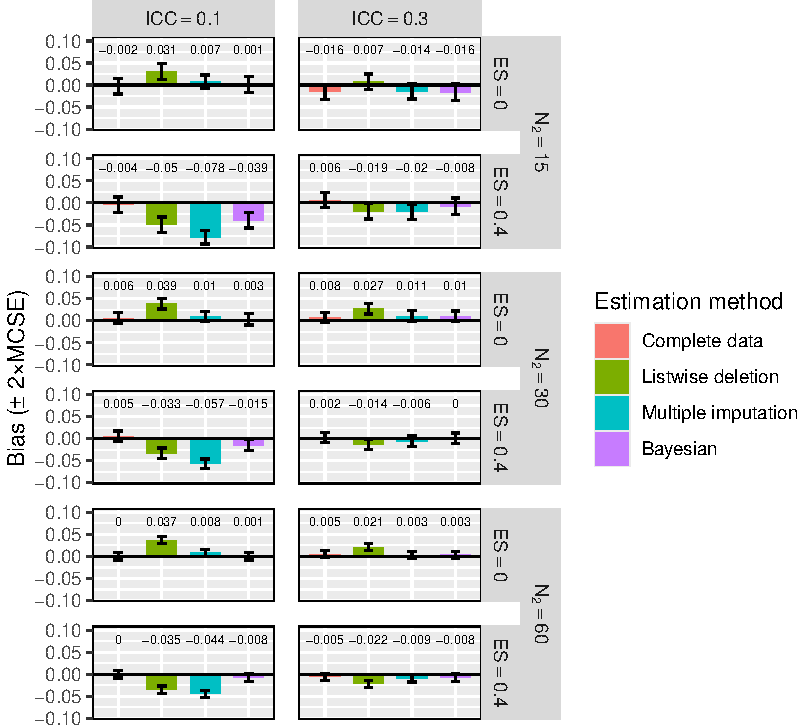
\includegraphics[width=1\linewidth,height=\textheight,keepaspectratio]{chapters/results_files/figure-pdf/fig-bias-1.pdf}

}

\caption[Bias of \(\gamma_{01}\) across simulation conditions under
MAR.]{\label{fig-bias}Bias of the between-group effect \(\gamma_{01}\)
across simulation conditions under missing at random (MAR). Error bars
represent ±2 Monte Carlo standard errors (MCSE). ES = effect size; ICC =
intraclass correlation coefficient used for both the residual ICC of
\(Y\) and the ICC of \(X\); \(N_2\) = number of groups.}

\end{figure}%

\section{Coverage of confidence and credible
intervals}\label{coverage-of-confidence-and-credible-intervals}

The results for coverage of the confidence and credible intervals for
\(\gamma_{01}\) are shown for \(N_2 = 15\) in Figure~\ref{fig-cov}, as
larger sample sizes exhibited similar but attenuated patterns. Overall,
coverage rates were close to the nominal level (95\%) for \(N_2 = 30\)
and \(N_2 = 60\) across all methods. LD yielded coverage rates close to
the nominal level in all conditions. For multiple imputation, coverage
in the MI-R variant was close to the nominal level in high-ICC
conditions, with a tendency toward overcoverage in low-ICC conditions.
For \(ICC = .1\), coverage ranged from 0.952 (\(N_2 = 30\),
\(\gamma_{01} = 0.4\), MAR) to 0.971 (\(N_2 = 60\), \(\gamma_{01} = 0\),
MCAR). The approach using small-sample adjusted degrees of freedom
resulted in increased overcoverage compared to the standard degrees of
freedom, particularly for \(N_2 = 15\). Overcoverage was again more
pronounced in low-ICC conditions, ranging from 0.960 (\(N_2 = 60\),
\(\gamma_{01} = 0.4\), MCAR) to 0.986 (\(N_2 = 15\),
\(\gamma_{01} = 0\), MCAR) for \(ICC = .1\).\\
The Bayesian approach exhibited overcoverage for \(N_2 = 15\), ranging
from 0.963 (\(\gamma_{01} = 0\), MCAR, \(ICC = .1\)) to 0.985
(\(\gamma_{01} = 0.4\), MCAR, \(ICC = .1\)). This method yielded the
highest (most conservative) coverage rates at the smallest level-2
sample size, except in the condition with MCAR, \(ICC = .1\), and
\(\gamma_{01} = 0\). With increasing level-2 sample size, this pattern
attenuated. For \(N_2 = 30\), coverage estimates were largely within the
bounds of Monte Carlo error, and for \(N_2 = 60\), they fell entirely
within these bounds across all conditions.

\begin{figure}

\centering{

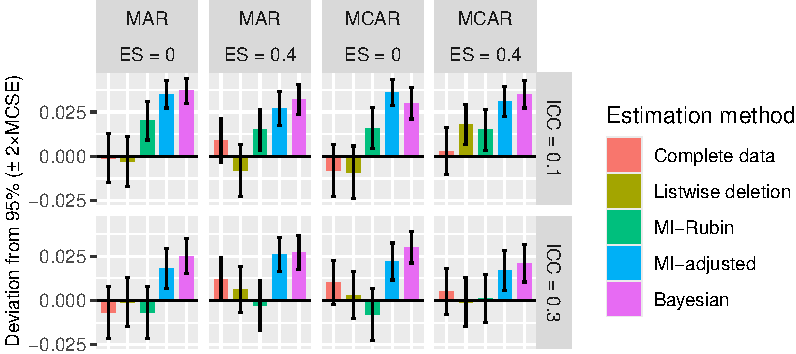
\includegraphics[width=1\linewidth,height=\textheight,keepaspectratio]{chapters/results_files/figure-pdf/fig-cov-1.pdf}

}

\caption[Coverage performance for \(N_2=15\)]{\label{fig-cov}Deviation
from nominal (95\%) coverage of confidence/credible intervals across
methods and simulation conditions for \(N_2 = 15\). Error bars represent
±2 Monte Carlo standard errors (MCSE). ES = effect size; MAR = missing
at random; MCAR = missing completely at random; ICC = intraclass
correlation coefficient used for both the residual ICC of \(Y\) and the
ICC of \(X\); MI-Rubin = multiple imputation using Rubin's degrees of
freedom; MI-adjusted = multiple imputation using adjusted degrees of
freedom.}

\end{figure}%

\section{Standard deviation of point
estimates}\label{standard-deviation-of-point-estimates}

Standard deviations of point estimates across conditions and methods are
illustrated in Figure~\ref{fig-sd} for MAR, as differences between
missingness mechanisms were small.

LD produced standard deviations very close to those obtained under CD,
ranging from 0.124 (\(N_2 = 60\), MCAR, \(\gamma_{01} = 0.4\)) to 0.300
(\(N_2 = 15\), MCAR, \(\gamma_{01} = 0\)). For MI, standard deviations
were comparable to CD across conditions, with a tendency toward smaller
values in some low-ICC conditions. For example, for \(N_2 = 15\),
\(\gamma_{01} = 0\), and MAR missingness, MI yielded a standard
deviation of 0.247, compared to 0.283 under CD. The Bayesian approach
yielded standard deviations that were generally slightly larger than
those from complete-data analysis, typically by approximately 0.006 to
0.020. Standard deviations were generally smaller under high ICC
conditions than under low ICC conditions in the Bayesian framework,
except in the conditions with \(\gamma_{01} = 0.4\) and \(N_2 = 15\). In
contrast, MI consistently yielded slightly larger standard deviations
under high-ICC conditions. Although these differences were small, they
were larger than would be expected from Monte Carlo error alone.

\begin{figure}

\centering{

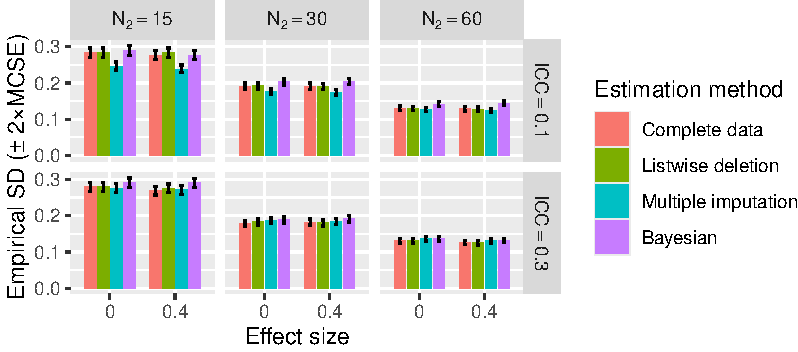
\includegraphics[width=1\linewidth,height=\textheight,keepaspectratio]{chapters/results_files/figure-pdf/fig-sd-1.pdf}

}

\caption[Empirical standard deviations for \(\gamma_{01}\) under
MAR]{\label{fig-sd}Empirical standard deviation (SD) of point estimates
for \(\gamma_{01}\) for conditions with missingness at random (MAR).
Error bars represent ±2 Monte Carlo standard errors (MCSE). \(N_2\) =
number of groups; ICC = intraclass correlation coefficient used for both
the residual ICC of \(Y\) and the ICC of \(X\).}

\end{figure}%

\section{Width of confidence and credible
intervals}\label{width-of-confidence-and-credible-intervals}

Results for the width of confidence and credible intervals are
illustrated in Figure~\ref{fig-ciw}, as similar patterns were observed
across conditions. Overall, the Bayesian approach yielded the widest
credible intervals, followed by multiple imputation with adjusted
degrees of freedom (MI-a). For \(N_2 = 15\), the MI-R variant produced
interval widths that were slightly smaller than those obtained under CD
(e.g., 1.115 vs.~1.170 for MCAR, \(ICC = .1\), \(\gamma_{01} = 0\)). For
\(N_2 = 30\) and \(N_2 = 60\), MI-R interval widths were slightly larger
than those from CD, while still remaining smaller than those from MI-a
and the Bayesian approach. Confidence intervals from LD were similar to
those obtained with CD across conditions.\\
At the smallest level-2 sample size, \(N_2 = 15\), differences between
methods were most pronounced. For example, when \(\gamma_{01} = 0\) and
\(ICC = .1\) under MCAR, interval width for \(\gamma_{01}\) was 1.115
under MI-R, 1.284 with MI-a and 1.456 under the Bayesian approach. With
increasing level-2 sample size, differences between methods became less
pronounced, although interval widths for the Bayesian approach remained
slightly larger. For instance, when \(\gamma_{01} = 0\), \(ICC = .1\),
and MCAR at \(N_2 = 60\), interval width was 0.517 for complete-data
analysis, 0.520 for LD, 0.545 for MI-R, 0.559 for MI-a, and 0.582 for
the Bayesian approach. Within the fully Bayesian approach, interval
widths were generally slightly smaller under high-ICC conditions than
under low-ICC conditions. In contrast, the other methods did not show a
consistent ICC-related pattern.

\begin{figure}

\centering{

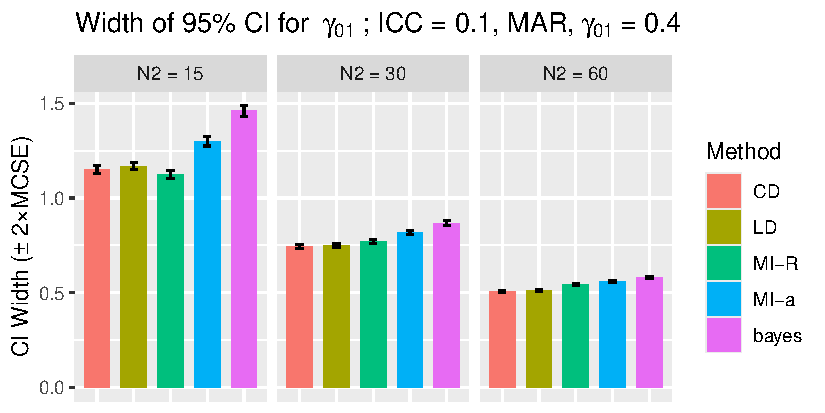
\includegraphics[width=1\linewidth,height=\textheight,keepaspectratio]{chapters/results_files/figure-pdf/fig-ciw-1.pdf}

}

\caption[Width of confidence/credible intervals for
\(\gamma_{01}=0.40\)]{\label{fig-ciw}Width of confidence/credible
intervals for \(\gamma_{01} = 0.40\) under missing at random (MAR) and
\(ICC = .10\), where ICC denotes the intraclass correlation coefficient
used for both the residual ICC of \(Y\) and the ICC of \(X\). Error bars
represent ±2 Monte Carlo standard errors (MCSE). \(N_2\) = number of
groups; MI-Rubin = multiple imputation with Rubin's degrees of freedom;
MI-adjusted = multiple imputation with small-sample-adjusted degrees of
freedom.}

\end{figure}%

\section{Summary of results}\label{summary-of-results}

The methods showed different performance profiles for the level-2
effect. LD resulted in increased bias, while other performance measures
were generally similar to CD results. MI produced substantial downward
bias in the estimation of the level-2 effect under conditions of low ICC
and MAR missingness. At the same time, the standard variant (MI-R)
yielded coverage rates close to the nominal level across conditions.
Applying a small-sample correction to the degrees of freedom led to
increased coverage beyond the nominal level and wider confidence
intervals. The fully Bayesian approach showed small to negligible bias
across conditions, but resulted in the widest intervals among all
methods and a tendency toward overcoverage in the smallest sample size.

\bookmarksetup{startatroot}

\chapter{Discussion}\label{discussion}

This thesis investigated the performance of two modern methods for
handling missing predictor data in small-sample multilevel models,
multiple imputation and a fully Bayesian approach, alongside listwise
deletion as a commonly used default. It focused on a reduced setting
with a single continuous predictor which was included at level 1 as an
individual-level predictor and at level 2 as a manifest group-mean
predictor, within a random intercept model. In addition, one auxiliary
variable at level 2 was included to explain missingness under a MAR
mechanism, without being directly related to the outcome.

The results indicate a trade-off between bias and interval width when
comparing multiple imputation and the fully Bayesian approach. In
settings with low ICC and default prior specifications, the fully
Bayesian approach may offer advantages over multiple imputation with
respect to bias, with differences persisting even at comparatively
larger cluster sizes in the present design. Although multiple imputation
can be understood as an approximate Bayesian procedure, as it relies on
draws from the posterior predictive distribution (e.g.,
\citeproc{ref-endersbook}{Enders, 2022, p. 299};
\citeproc{ref-SG2002}{Schafer \& Graham, 2002}), the present results
suggest that this connection does not necessarily translate into
comparable performance in small samples. In particular, prior
specification played an important role, as indicated by the sensitivity
analysis. When reasonable prior information is available for level-2
variance components, incorporating this information through weakly
informative priors can reduce bias in multiple imputation while holding
coverage at a nominal level.

Another aspect of multiple imputation that was specifically investigated
in this thesis is the behavior of inference based on uncorrected versus
small-sample-adjusted degrees of freedom. The findings suggest that, in
this setting, standard Rubin's rules already yield approximately valid
inference, and that additional small-sample corrections may not be
necessary. This is somewhat surprising, as it is commonly recommended to
use an appropriate sampling distribution in small samples to avoid
overly narrow confidence intervals; a recommendation which also applies
to multilevel analyses (\citeproc{ref-kenwardroger}{Kenward \& Roger,
1997}; \citeproc{ref-schaalje}{Schaalje et al., 2002}) and within
multiple imputation (\citeproc{ref-barnard}{Barnard \& Rubin, 1999}).
However, confidence intervals are influenced by multiple sources of
uncertainty beyond the degrees-of-freedom approximation alone. In
particular, REML estimation was used for analyzing the imputed data
sets. Compared to ML, REML typically yields larger estimates of level-2
variance components, which have been shown to improve variance
estimation in small samples (\citeproc{ref-elff}{Elff et al., 2021};
\citeproc{ref-mcneishstaple14}{McNeish \& Stapleton, 2016b}). As these
variance components directly affect the standard errors of the fixed
effects, they also influence the within-imputation variance and,
consequently, the total variance used for inference. This may have
contributed to wider intervals and thus higher coverage. In addition,
multiple imputation was performed using joint modeling via
\texttt{jomo}. Previous work has shown that inverse Wishart priors with
few degrees of freedom, as implemented in \texttt{jomo}, can introduce
additional variability into fixed-effect estimates
(\citeproc{ref-audigier}{Audigier et al., 2018}). Overall, this finding
may be reassuring for applied researchers relying on default
degrees-of-freedom specifications.\\
In terms of implementation, both fully Bayesian estimation and multiple
imputation allow the inclusion of auxiliary variables, which were also
part of the present setup. In multiple imputation, their inclusion is
typically well-documented and supported by standard workflows. In fully
Bayesian approaches, however, incorporating auxiliary variables without
altering the analysis model requires additional modeling decisions that
are less explicitly supported by standardized workflows and software
guidance and may therefore not be as straightforward to practitioners.
Against this background, the choice between approaches is likely to
depend not only on statistical performance but also on the research
context and analytical goals. Multiple imputation may be advantageous in
settings involving multiple analyses (e.g., multiple outcomes), where
standardized workflows and comparability across analyses are desired, as
completed data sets can be reused and shared. In contrast, fully
Bayesian approaches may be particularly useful in cumulative research
settings, where prior information can be updated across studies and
evidence can be built up and integrated over time
(\citeproc{ref-vandeschoot}{Van De Schoot et al., 2014}). However, these
distinctions are not absolute, and both approaches can, in principle, be
adapted to a wide range of analytical scenarios.

This simulation study comes with several limitations. Firstly, more
complex model structures may behave differently under the investigated
methods. The present study focused on a relatively simple model without
nonlinear terms, interaction effects, or random slopes. Sample size
requirements in multilevel models generally depend on model complexity,
as more complex specifications involve a larger number of parameters
that must be estimated reliably (\citeproc{ref-hoxcap}{Hox \& McNeish,
2020}). Therefore, what worked well in the present study might be more
problematic in more complex models. In particular, when such features
are present, the treatment of missing data becomes substantially more
challenging (\citeproc{ref-enders16}{Enders et al., 2016};
\citeproc{ref-grundRS}{Grund et al., 2016a},
\citeproc{ref-grundMI18}{2018b}). For multiple imputation, default
imputation models often lead to incompatibility between the imputation
and analysis model and, consequently, biased estimates
(\citeproc{ref-bartlett}{Bartlett et al., 2015}; \citeproc{ref-kim}{Kim
et al., 2018}; \citeproc{ref-seamanMI}{Seaman et al., 2012}). Therefore,
approaches that allow for substantive-model-compatible MI, such as
sequential modeling, have been proposed to address these challenges
(\citeproc{ref-bartlett}{Bartlett et al., 2015};
\citeproc{ref-endersmodel}{Enders et al., 2020};
\citeproc{ref-grundMImdmb}{Grund et al., 2021};
\citeproc{ref-luedtke20}{Lüdtke et al., 2020};
\citeproc{ref-zhangwang}{Zhang \& Wang, 2017}), but these approaches
have not yet been thoroughly investigated in data sets with few
clusters.\\
Second, the present results may not generalize to more extreme
small-sample settings. With very few clusters, for example fewer than
10, variance components are difficult to estimate reliably, which can
affect both multiple imputation and Bayesian approaches
(\citeproc{ref-hox}{Hox et al., 2012}; \citeproc{ref-maashox}{Maas \&
Hox, 2005}; \citeproc{ref-mcneish}{McNeish \& Stapleton, 2016a}).
Furthermore, cluster size plays an important role for estimation and was
fixed at 10 in the present study. With very few observations per cluster
and unbalanced data (i.e., unequal number of observations per cluster),
different patterns of results might be obtained; e.g., very small
cluster sizes are connected to an upward bias in level-2 variance
components if number of groups was also small
(\citeproc{ref-clarke}{Clarke, 2008}; \citeproc{ref-mcneishlv1}{McNeish,
2014}). Empirical evidence on the effects of unbalanced cluster sizes is
sparse, but existing literature suggests that they can bias statistical
inference by leading to underestimated standard errors of fixed effects,
particularly when combined with heteroscedasticity and a small number of
clusters (\citeproc{ref-korendijk}{Korendijk et al., 2008};
\citeproc{ref-raudenbush}{Raudenbush \& Bryk, 2010, p. 281}). Unbalanced
data also have implications for the imputation design in contextual
models. In such settings, imputation models that rely on manifest group
means and don't account for cluster size may introduce additional bias
(\citeproc{ref-grundlv2}{Grund et al., 2018a}).\\
Third, prior specification was only examined in a limited sensitivity
analysis for multiple imputation in the present study. In complete-data
settings, previous research suggests that weakly informative priors
often outperform noninformative priors in Bayesian multilevel models
with few clusters (\citeproc{ref-gelmanprior}{Gelman, 2006};
\citeproc{ref-mcneishbay}{McNeish, 2016a}; \citeproc{ref-smid}{Smid et
al., 2020}), whereas findings on data-dependent priors remain
inconclusive (\citeproc{ref-depaoli13}{Depaoli, 2013};
\citeproc{ref-mcneishpriors}{McNeish, 2016b}; \citeproc{ref-erp}{Van Erp
et al., 2018}). However, studies on the role of prior specification in
the presence of missing data and few clusters remain sparse. For
multiple imputation in particular, standard software priors are often
used, although some findings suggest that prior choice can substantially
influence results in multiple imputation as well
(\citeproc{ref-audigier}{Audigier et al., 2018};
\citeproc{ref-grundMI18}{Grund et al., 2018b}). Extending this line of
research to settings with missing data would therefore be an important
direction for future research.\\
Fourth, several key modeling choices were not systematically varied in
the present study. Future research could manipulate estimation methods
(ML versus REML), imputation frameworks (joint modeling versus fully
conditional specification), small-sample corrections (e.g.,
Kenward-Roger, \(m−l−1\)), prior specifications and model complexity to
disentangle their relative contributions to estimation performance. Such
work would help clarify the behavior of multiple imputation in
comparison with fully Bayesian estimation and identify the conditions
under which small-sample corrections for degrees of freedom are useful,
as well as those under which they may not be necessary. Existing
evidence suggests that degree-of-freedom corrections might be beneficial
in more complex models, such as growth models with random slopes and
longitudinal missingness patterns (\citeproc{ref-mcneishgrowth}{McNeish,
2018}).\\
Fifth, two distinct software packages with different default prior
specifications were used for multiple imputation and Bayesian
estimation. Using a common software framework for both approaches, as
for example possible with \texttt{mdmb}
(\citeproc{ref-grundMImdmb}{Grund et al., 2021};
\citeproc{ref-mdmb}{Robitzsch \& Luedtke, 2024}), could improve
comparability and help isolate differences attributable to modeling
choices rather than implementation details.

Finally, a further limitation concerns the missing data mechanism. The
present study assumes missingness (completely) at random, whereas the
combination of few clusters and missing data should also be investigated
under missingness not at random, which requires different modeling
approaches (\citeproc{ref-duMNAR}{Du et al., 2022};
\citeproc{ref-endersupdate}{Enders, 2025}). Moreover, the present
missingness pattern with missings only in one predictor variable is very
simplified, as in real-world applications, missing values typically
occur across multiple variables, including outcomes, level-1 and level-2
predictors, and the grouping variable (\citeproc{ref-buuren}{Van Buuren,
2018}). Even if the joint modeling approach used in this thesis can
accommodate multivariate missings, bias and efficiency of the estimates
might be differently affected by different model specifications.

Overall, the present findings provide insight into the behavior of
missing data methods in small-sample multilevel settings with missings
in a predictor variable, but further research is required to assess
their robustness under more complex and realistic conditions.

\bookmarksetup{startatroot}

\chapter*{References}\label{references}
\addcontentsline{toc}{chapter}{References}

\markboth{References}{References}

\phantomsection\label{refs}
\begin{CSLReferences}{1}{0}
\bibitem[\citeproctext]{ref-aarts}
Aarts, E., Verhage, M., Veenvliet, J. V., Dolan, C. V., \& Van Der
Sluis, S. (2014). A solution to dependency: Using multilevel analysis to
accommodate nested data. \emph{Nature Neuroscience}, \emph{17}(4),
491--496. \url{https://doi.org/10.1038/nn.3648}

\bibitem[\citeproctext]{ref-aguinis}
Aguinis, H., Gottfredson, R. K., \& Culpepper, S. A. (2013).
Best-practice recommendations for estimating cross-level interaction
effects using multilevel modeling. \emph{Journal of Management},
\emph{39}(6), 1490--1528. \url{https://doi.org/10.1177/0149206313478188}

\bibitem[\citeproctext]{ref-anderman}
Anderman, E. M. (2002). School effects on psychological outcomes during
adolescence. \emph{Journal of Educational Psychology}, \emph{94}(4),
795--809. \url{https://doi.org/10.1037/0022-0663.94.4.795}

\bibitem[\citeproctext]{ref-mdmbprior}
Asparouhov, T., \& Muthen, B. (2010). \emph{Bayesian analysis using
{Mplus}: {Technical} implementation}.

\bibitem[\citeproctext]{ref-audigier}
Audigier, V., White, I. R., Jolani, S., Debray, T. P. A., Quartagno, M.,
Carpenter, J., Van Buuren, S., \& Resche-Rigon, M. (2018). Multiple
imputation for multilevel data with continuous and binary variables.
\emph{Statistical Science}, \emph{33}(2).
\url{https://doi.org/10.1214/18-STS646}

\bibitem[\citeproctext]{ref-barnard}
Barnard, J., \& Rubin, D. (1999). Small-sample degrees of freedom with
multiple imputation. \emph{Biometrika}, \emph{86}(4), 948--955.

\bibitem[\citeproctext]{ref-bartlett}
Bartlett, J. W., Seaman, S. R., White, I. R., Carpenter, J. R., \& for
the Alzheimer's Disease Neuroimaging Initiative*. (2015). Multiple
imputation of covariates by fully conditional specification:
{Accommodating} the substantive model. \emph{Statistical Methods in
Medical Research}, \emph{24}(4), 462--487.
\url{https://doi.org/10.1177/0962280214521348}

\bibitem[\citeproctext]{ref-clarke}
Clarke, P. (2008). When can group level clustering be ignored?
{Multilevel} models versus single-level models with sparse data.
\emph{Journal of Epidemiology and Community Health}, \emph{62}(8),
752--758. \url{https://doi.org/10.1136/jech.2007.060798}

\bibitem[\citeproctext]{ref-collins}
Collins, L. M., Schafer, J. L., \& Kam, C.-M. (2001). A comparison of
inclusive and restrictive strategies in modern missing data procedures.
\emph{Psychological Methods}, \emph{6}(4), 330--351.
\url{https://doi.org/10.1037/1082-989X.6.4.330}

\bibitem[\citeproctext]{ref-croon}
Croon, M. A., \& Van Veldhoven, M. J. P. M. (2007). Predicting
group-level outcome variables from variables measured at the individual
level: {A} latent variable multilevel model. \emph{Psychological
Methods}, \emph{12}(1), 45--57.
\url{https://doi.org/10.1037/1082-989X.12.1.45}

\bibitem[\citeproctext]{ref-daniels}
Daniels, M. J., Wang, C., \& Marcus, B. H. (2014). Fully {Bayesian}
inference under ignorable missingness in the presence of auxiliary
covariates. \emph{Biometrics}, \emph{70}(1), 62--72.
\url{https://doi.org/10.1111/biom.12121}

\bibitem[\citeproctext]{ref-depaoli13}
Depaoli, S. (2013). Mixture class recovery in {GMM} under varying
degrees of class separation: {Frequentist} versus {Bayesian} estimation.
\emph{Psychological Methods}, \emph{18}(2), 186--219.
\url{https://doi.org/10.1037/a0031609}

\bibitem[\citeproctext]{ref-depaoli}
Depaoli, S., \& Clifton, J. P. (2015). A {Bayesian} approach to
multilevel structural equation modeling with continuous and dichotomous
outcomes. \emph{Structural Equation Modeling: A Multidisciplinary
Journal}, \emph{22}(3), 327--351.
\url{https://doi.org/10.1080/10705511.2014.937849}

\bibitem[\citeproctext]{ref-duMNAR}
Du, H., Enders, C., Keller, B. T., Bradbury, T. N., \& Karney, B. R.
(2022). A {Bayesian} latent variable selection model for nonignorable
missingness. \emph{Multivariate Behavioral Research}, \emph{57}(2-3),
478--512. \url{https://doi.org/10.1080/00273171.2021.1874259}

\bibitem[\citeproctext]{ref-elff}
Elff, M., Heisig, J. P., Schaeffer, M., \& Shikano, S. (2021).
Multilevel analysis with few clusters: {Improving} likelihood-based
methods to provide unbiased estimates and accurate inference.
\emph{British Journal of Political Science}, \emph{51}(1), 412--426.
\url{https://doi.org/10.1017/S0007123419000097}

\bibitem[\citeproctext]{ref-endersbook}
Enders, C. K. (2022). \emph{Applied missing data analysis} (2nd ed).
Guilford Press.

\bibitem[\citeproctext]{ref-endersupdate}
Enders, C. K. (2025). Missing data: {An} update on the state of the art.
\emph{Psychological Methods}, \emph{30}(2), 322--339.
\url{https://doi.org/10.1037/met0000563}

\bibitem[\citeproctext]{ref-endersmodel}
Enders, C. K., Du, H., \& Keller, B. T. (2020). A model-based imputation
procedure for multilevel regression models with random coefficients,
interaction effects, and nonlinear terms. \emph{Psychological Methods},
\emph{25}(1), 88--112. \url{https://doi.org/10.1037/met0000228}

\bibitem[\citeproctext]{ref-enders16}
Enders, C. K., Mistler, S. A., \& Keller, B. T. (2016). Multilevel
multiple imputation: A review and evaluation of joint modeling and
chained equations imputation. \emph{Psychological Methods},
\emph{21}(2), 222--240. \url{https://doi.org/10.1037/met0000063}

\bibitem[\citeproctext]{ref-erler}
Erler, N. S., Rizopoulos, D., Rosmalen, J. V., Jaddoe, V. W. V., Franco,
O. H., \& Lesaffre, E. M. E. H. (2016). Dealing with missing covariates
in epidemiologic studies: A comparison between multiple imputation and a
full {Bayesian} approach. \emph{Statistics in Medicine}, \emph{35}(17),
2955--2974. \url{https://doi.org/10.1002/sim.6944}

\bibitem[\citeproctext]{ref-fahrmeir}
Fahrmeir, L., Kneib, T., Lang, S., \& Marx, B. D. (2021).
\emph{Regression: {Models}, methods and applications}. Springer Berlin
Heidelberg. \url{https://doi.org/10.1007/978-3-662-63882-8}

\bibitem[\citeproctext]{ref-gelmanprior}
Gelman, A. (2006). Prior distributions for variance parameters in
hierarchical models (comment on article by {Browne} and {Draper}).
\emph{Bayesian Analysis}, \emph{1}(3).
\url{https://doi.org/10.1214/06-BA117A}

\bibitem[\citeproctext]{ref-gelmanbook}
Gelman, A., Carlin, J. B., Stern, H. S., Dunson, D. B., Vehtari, A., \&
Rubin, D. B. (2025). \emph{Bayesian data analysis third edition (with
errors fixed as of 20 february 2025)} (3rd ed.).

\bibitem[\citeproctext]{ref-gelmanrhat}
Gelman, A., \& Rubin, D. B. (1992). Inference from iterative simulation
using multiple sequences. \emph{Statistical Science}, \emph{7}(4).
\url{https://doi.org/10.1214/ss/1177011136}

\bibitem[\citeproctext]{ref-grahamFIML}
Graham, J. W. (2003). Adding missing-data-relevant variables to
{FIML-based} structural equation models. \emph{Structural Equation
Modeling: A Multidisciplinary Journal}, \emph{10}(1), 80--100.
\url{https://doi.org/10.1207/S15328007SEM1001_4}

\bibitem[\citeproctext]{ref-graham09}
Graham, J. W. (2009). Missing data analysis: {Making} it work in the
real world. \emph{Annual Review of Psychology}, \emph{60}(1), 549--576.
\url{https://doi.org/10.1146/annurev.psych.58.110405.085530}

\bibitem[\citeproctext]{ref-graham07}
Graham, J. W., Olchowski, A. E., \& Gilreath, T. D. (2007). How many
imputations are really needed? {Some} practical clarifications of
multiple imputation theory. \emph{Prevention Science}, \emph{8}(3),
206--213. \url{https://doi.org/10.1007/s11121-007-0070-9}

\bibitem[\citeproctext]{ref-grundRS}
Grund, S., Lüdtke, O., \& Robitzsch, A. (2016a). Multiple imputation of
missing covariate values in multilevel models with random slopes: A
cautionary note. \emph{Behavior Research Methods}, \emph{48}(2),
640--649. \url{https://doi.org/10.3758/s13428-015-0590-3}

\bibitem[\citeproctext]{ref-grundMI16}
Grund, S., Lüdtke, O., \& Robitzsch, A. (2016b). Multiple imputation of
multilevel missing data: {An} introduction to the {R} package pan.
\emph{Sage Open}, \emph{6}(4), 2158244016668220.
\url{https://doi.org/10.1177/2158244016668220}

\bibitem[\citeproctext]{ref-grundlv2}
Grund, S., Lüdtke, O., \& Robitzsch, A. (2018a). Multiple {Imputation}
of {Missing Data} at {Level} 2: {A Comparison} of {Fully Conditional}
and {Joint Modeling} in {Multilevel Designs}. \emph{Journal of
Educational and Behavioral Statistics}, \emph{43}(3), 316--353.
\url{https://doi.org/10.3102/1076998617738087}

\bibitem[\citeproctext]{ref-grundMI18}
Grund, S., Lüdtke, O., \& Robitzsch, A. (2018b). Multiple imputation of
missing data for multilevel models: {Simulations} and recommendations.
\emph{Organizational Research Methods}, \emph{21}(1), 111--149.
\url{https://doi.org/10.1177/1094428117703686}

\bibitem[\citeproctext]{ref-grundapa}
Grund, S., Lüdtke, O., \& Robitzsch, A. (2019). Missing data in
multilevel research. In S. E. Humphrey \& J. M. LeBreton (Eds.),
\emph{The handbook of multilevel theory, measurement, and analysis.}
(pp. 365--386). American Psychological Association.
\url{https://doi.org/10.1037/0000115-017}

\bibitem[\citeproctext]{ref-grundMImdmb}
Grund, S., Lüdtke, O., \& Robitzsch, A. (2021). Multiple imputation of
missing data in multilevel models with the {R} package mdmb: A flexible
sequential modeling approach. \emph{Behavior Research Methods},
\emph{53}(6), 2631--2649.
\url{https://doi.org/10.3758/s13428-020-01530-0}

\bibitem[\citeproctext]{ref-mitml}
Grund, S., Robitzsch, A., \& Luedtke, O. (2015). \emph{Mitml: {Tools}
for multiple imputation in multilevel modeling} (pp. 0.4--5).
Comprehensive R Archive Network.
\url{https://doi.org/10.32614/CRAN.package.mitml}

\bibitem[\citeproctext]{ref-heisig}
Heisig, J. P., \& Schaeffer, M. (2019). Why you should {\emph{Always}}
include a random slope for the lower-level variable involved in a
cross-level interaction. \emph{European Sociological Review},
\emph{35}(2), 258--279. \url{https://doi.org/10.1093/esr/jcy053}

\bibitem[\citeproctext]{ref-holtmann}
Holtmann, J., Koch, T., Lochner, K., \& Eid, M. (2016). A comparison of
{ML}, {WLSMV}, and {Bayesian} methods for multilevel structural equation
models in small samples: A simulation study. \emph{Multivariate
Behavioral Research}, \emph{51}(5), 661--680.
\url{https://doi.org/10.1080/00273171.2016.1208074}

\bibitem[\citeproctext]{ref-hoxcap}
Hox, J. J., \& McNeish, D. (2020). Small {Samples} in {Multilevel
Modeling}. In \emph{Small {Sample Size Solutions}} (1st ed., pp.
215--225). Routledge. \url{https://doi.org/10.4324/9780429273872-18}

\bibitem[\citeproctext]{ref-hox}
Hox, J. J., Van De Schoot, R., \& Matthijsse, S. (2012). How few
countries will do? {Comparative} survey analysis from a {Bayesian}
perspective. \emph{Survey Research Methods}, \emph{Vol 6}, 87--93 Pages.
\url{https://doi.org/10.18148/SRM/2012.V6I2.5033}

\bibitem[\citeproctext]{ref-johnson}
Johnson, A. A., Ott, M. Q., \& Dogucu, M. (2022). \emph{Bayes rules!:
{An} introduction to applied {Bayesian} modeling} (1st ed.). {Chapman
and Hall/CRC}. \url{https://doi.org/10.1201/9780429288340}

\bibitem[\citeproctext]{ref-kackar}
Kackar, R. N., \& Harville, D. A. (1981). Unbiasedness of two-stage
estimation and prediction procedures for mixed linear models.
\emph{Communications in Statistics - Theory and Methods}, \emph{10}(13),
1249--1261. \url{https://doi.org/10.1080/03610928108828108}

\bibitem[\citeproctext]{ref-kackarcorr}
Kackar, R. N., \& Harville, D. A. (1984). Approximations for standard
errors of estimators of fixed and random effect in mixed linear models.
\emph{Journal of the American Statistical Association}, \emph{79}(388),
853. \url{https://doi.org/10.2307/2288715}

\bibitem[\citeproctext]{ref-kadane}
Kadane, J. B. (2015). Bayesian {Methods} for {Prevention Research}.
\emph{Prevention Science}, \emph{16}(7), 1017--1025.
\url{https://doi.org/10.1007/s11121-014-0531-x}

\bibitem[\citeproctext]{ref-kahan}
Kahan, B. C., Forbes, G., Ali, Y., Jairath, V., Bremner, S., Harhay, M.
O., Hooper, R., Wright, N., Eldridge, S. M., \& Leyrat, C. (2016).
Increased risk of type {I} errors in cluster randomised trials with
small or medium numbers of clusters: A review, reanalysis, and
simulation study. \emph{Trials}, \emph{17}(1), 438.
\url{https://doi.org/10.1186/s13063-016-1571-2}

\bibitem[\citeproctext]{ref-kenwardroger}
Kenward, M. G., \& Roger, J. H. (1997). Small sample inference for fixed
effects from restricted maximum likelihood. \emph{Biometrics},
\emph{53}(3), 983. \url{https://doi.org/10.2307/2533558}

\bibitem[\citeproctext]{ref-kim}
Kim, S., Belin, T. R., \& Sugar, C. A. (2018). Multiple imputation with
non-additively related variables: {Joint-modeling} and approximations.
\emph{Statistical Methods in Medical Research}, \emph{27}(6),
1683--1694. \url{https://doi.org/10.1177/0962280216667763}

\bibitem[\citeproctext]{ref-korendijk}
Korendijk, E. J. H., Maas, C. J. M., Moerbeek, M., \& Van Der Heijden,
P. G. M. (2008). The {Influence} of {Misspecification} of the
{Heteroscedasticity} on {Multilevel Regression Parameter} and {Standard
Error Estimates}. \emph{Methodology}, \emph{4}(2), 67--72.
\url{https://doi.org/10.1027/1614-2241.4.2.67}

\bibitem[\citeproctext]{ref-leonhart}
Leonhart, R. (2013). \emph{{Lehrbuch Statistik: Einstieg und
Vertiefung}} (3., überarbeitete und erweiterte Auflage). Verlag Hans
Huber.

\bibitem[\citeproctext]{ref-littlerubin87}
Little, R. J. A., \& Rubin, D. B. (1987). \emph{Statistical analysis
with missing data} (3. {[}Dr.{]}). Wiley.

\bibitem[\citeproctext]{ref-little20}
Little, R. J. A., \& Rubin, D. B. (2020). \emph{Statistical analysis
with missing data} (3rd edition). Wiley.
\url{https://doi.org/10.1002/9781119482260}

\bibitem[\citeproctext]{ref-luedtkecontext}
Lüdtke, O., Marsh, H. W., Robitzsch, A., Trautwein, U., Asparouhov, T.,
\& Muthén, B. (2008). The multilevel latent covariate model: {A} new,
more reliable approach to group-level effects in contextual studies.
\emph{Psychological Methods}, \emph{13}(3), 203--229.
\url{https://doi.org/10.1037/a0012869}

\bibitem[\citeproctext]{ref-luedtkeMI}
Lüdtke, O., Robitzsch, A., \& Grund, S. (2017). Multiple imputation of
missing data in multilevel designs: A comparison of different
strategies. \emph{Psychological Methods}, \emph{22}(1), 141--165.
\url{https://doi.org/10.1037/met0000096}

\bibitem[\citeproctext]{ref-luedtke}
Lüdtke, O., Robitzsch, A., Trautwein, U., \& Köller, O. (2007). {Umgang
mit fehlenden Werten in der psychologischen Forschung}.
\emph{Psychologische Rundschau}, \emph{58}(2), 103--117.
\url{https://doi.org/10.1026/0033-3042.58.2.103}

\bibitem[\citeproctext]{ref-luedtke20}
Lüdtke, O., Robitzsch, A., \& West, S. G. (2020). Regression models
involving nonlinear effects with missing data: A sequential modeling
approach using {Bayesian} estimation. \emph{Psychological Methods},
\emph{25}(2), 157--181. \url{https://doi.org/10.1037/met0000233}

\bibitem[\citeproctext]{ref-maashox}
Maas, C. J. M., \& Hox, J. J. (2005). \emph{Sufficient {Sample Sizes}
for {Multilevel Modeling}}. \emph{1}.

\bibitem[\citeproctext]{ref-mcneishlv1}
McNeish, D. (2014). Modeling sparsely clustered data: {Design-based},
model-based, and single-level methods. \emph{Psychological Methods},
\emph{19}(4), 552--563. \url{https://doi.org/10.1037/met0000024}

\bibitem[\citeproctext]{ref-mcneishbay}
McNeish, D. (2016a). On using {Bayesian} methods to address small sample
problems. \emph{Structural Equation Modeling: A Multidisciplinary
Journal}, \emph{23}(5), 750--773.
\url{https://doi.org/10.1080/10705511.2016.1186549}

\bibitem[\citeproctext]{ref-mcneishpriors}
McNeish, D. (2016b). Using data-dependent priors to mitigate small
sample bias in latent growth models: A discussion and illustration using
{Mplus}. \emph{Journal of Educational and Behavioral Statistics},
\emph{41}(1), 27--56. \url{https://doi.org/10.3102/1076998615621299}

\bibitem[\citeproctext]{ref-mcneish17}
McNeish, D. (2017a). Missing data methods for arbitrary missingness with
small samples. \emph{Journal of Applied Statistics}, \emph{44}(1),
24--39. \url{https://doi.org/10.1080/02664763.2016.1158246}

\bibitem[\citeproctext]{ref-mcneishcoll}
McNeish, D. (2017b). Small sample methods for multilevel modeling: A
colloquial elucidation of {REML} and the {Kenward-Roger} correction.
\emph{Multivariate Behavioral Research}, \emph{52}(5), 661--670.
\url{https://doi.org/10.1080/00273171.2017.1344538}

\bibitem[\citeproctext]{ref-mcneishgrowth}
McNeish, D. (2018). Brief research report: {Growth} models with small
samples and missing data. \emph{The Journal of Experimental Education},
\emph{86}(4), 690--701.
\url{https://doi.org/10.1080/00220973.2017.1369384}

\bibitem[\citeproctext]{ref-mcneish}
McNeish, D., \& Stapleton, L. M. (2016a). Modeling clustered data with
very few clusters. \emph{Multivariate Behavioral Research},
\emph{51}(4), 495--518.
\url{https://doi.org/10.1080/00273171.2016.1167008}

\bibitem[\citeproctext]{ref-mcneishstaple14}
McNeish, D., \& Stapleton, L. M. (2016b). The effect of small sample
size on two-level model estimates: A review and illustration.
\emph{Educational Psychology Review}, \emph{28}(2), 295--314.
\url{https://doi.org/10.1007/s10648-014-9287-x}

\bibitem[\citeproctext]{ref-meng}
Meng, X.-L. (1994). Multiple-{Imputation Inferences} with {Uncongenial
Sources} of {Input}. \emph{Statistical Science}, \emph{9}(4).
\url{https://doi.org/10.1214/ss/1177010269}

\bibitem[\citeproctext]{ref-morris}
Morris, T. P., White, I. R., \& Crowther, M. J. (2019). Using simulation
studies to evaluate statistical methods. \emph{Statistics in Medicine},
\emph{38}(11), 2074--2102. \url{https://doi.org/10.1002/sim.8086}

\bibitem[\citeproctext]{ref-murray}
Murray, J. S. (2018). Multiple {Imputation}: {A Review} of {Practical}
and {Theoretical Findings}. \emph{Statistical Science}, \emph{33}(2).
\url{https://doi.org/10.1214/18-STS644}

\bibitem[\citeproctext]{ref-muthen12}
Muthén, B., \& Asparouhov, T. (2012). Bayesian structural equation
modeling: A more flexible representation of substantive theory.
\emph{Psychological Methods}, \emph{17}(3), 313--335.
\url{https://doi.org/10.1037/a0026802}

\bibitem[\citeproctext]{ref-nicholson}
Nicholson, J. S., Deboeck, P. R., \& Howard, W. (2017). Attrition in
developmental psychology: {A} review of modern missing data reporting
and practices. \emph{International Journal of Behavioral Development},
\emph{41}(1), 143--153. \url{https://doi.org/10.1177/0165025415618275}

\bibitem[\citeproctext]{ref-pandey}
Pandey, S., \& Bright, C. L. (2008). What are degrees of freedom?
\emph{Social Work Research}, \emph{32}(2), 119--128.
\url{https://doi.org/10.1093/swr/32.2.119}

\bibitem[\citeproctext]{ref-sport}
Papaioannou, A., Marsh, H. W., \& Theodorakis, Y. (2004). A multilevel
approach to motivational climate in physical education and sport
settings: {An} individual or a group level construct? \emph{Journal of
Sport and Exercise Psychology}, \emph{26}(1), 90--118.
\url{https://doi.org/10.1123/jsep.26.1.90}

\bibitem[\citeproctext]{ref-peugh}
Peugh, J. L., \& Enders, C. K. (2004). Missing data in educational
research: A review of reporting practices and suggestions for
improvement. \emph{Review of Educational Research}, \emph{74}(4),
525--556. \url{https://doi.org/10.3102/00346543074004525}

\bibitem[\citeproctext]{ref-jomo}
Quartagno, M., \& Carpenter, J. (2023). \emph{{jomo}: A package for
multilevel joint modelling multiple imputation}.

\bibitem[\citeproctext]{ref-r}
R Core Team. (2025). \emph{R: {A Language} and {Environment} for
{Statistical Computing}}. R Foundation for Statistical Computing.

\bibitem[\citeproctext]{ref-raudenbush}
Raudenbush, S., \& Bryk, A. S. (2010). \emph{Hierarchical linear models:
Applications and data analysis methods} (2. ed., {[}Nachdr.{]}). Sage
Publ.

\bibitem[\citeproctext]{ref-mdmb}
Robitzsch, A., \& Luedtke, O. (2024). \emph{Mdmb: {Model} based
treatment of missing data} (pp. 1.9--22). Comprehensive R Archive
Network. \url{https://doi.org/10.32614/CRAN.package.mdmb}

\bibitem[\citeproctext]{ref-rubin76}
Rubin, D. B. (1976). Inference and missing data. \emph{Biometrika},
\emph{63}(3), 581--592. \url{https://doi.org/10.1093/biomet/63.3.581}

\bibitem[\citeproctext]{ref-rubinbook87}
Rubin, D. B. (1987). \emph{Multiple imputation for nonresponse in
surveys}. Wiley. \url{https://doi.org/10.1002/9780470316696}

\bibitem[\citeproctext]{ref-schaalje}
Schaalje, G. B., McBride, J. B., \& Fellingham, G. W. (2002). Adequacy
of approximations to distributions of test statistics in complex mixed
linear models. \emph{Journal of Agricultural, Biological, and
Environmental Statistics}, \emph{7}(4), 512--524.
\url{https://doi.org/10.1198/108571102726}

\bibitem[\citeproctext]{ref-schafer03}
Schafer, J. L. (2003). Multiple imputation in multivariate problems when
the imputation and analysis models differ. \emph{Statistica
Neerlandica}, \emph{57}(1), 19--35.
\url{https://doi.org/10.1111/1467-9574.00218}

\bibitem[\citeproctext]{ref-SG2002}
Schafer, J. L., \& Graham, J. W. (2002). Missing data: {Our} view of the
state of the art. \emph{Psychological Methods}, \emph{7}(2), 147--177.
\url{https://doi.org/10.1037/1082-989X.7.2.147}

\bibitem[\citeproctext]{ref-seamanMI}
Seaman, S. R., Bartlett, J. W., \& White, I. R. (2012). Multiple
imputation of missing covariates with non-linear effects and
interactions: An evaluation of statistical methods. \emph{BMC Medical
Research Methodology}, \emph{12}(1), 46.
\url{https://doi.org/10.1186/1471-2288-12-46}

\bibitem[\citeproctext]{ref-shinshin}
Shin, D., \& Shin, Y. (2025). \emph{Compatible imputation for
hierarchical linear models with incomplete data: {Interaction} effects
of continuous and categorical covariates {MAR}} (arXiv:2502.07033).
arXiv. \url{https://doi.org/10.48550/arXiv.2502.07033}

\bibitem[\citeproctext]{ref-shin}
Shin, D., Shin, Y., \& Hagiwara, N. (2025). \emph{Bayesian estimation of
hierarchical linear models from incomplete data: {Cluster-level}
interaction effects and small sample sizes} (arXiv:2405.21020). arXiv.
\url{https://doi.org/10.48550/arXiv.2405.21020}

\bibitem[\citeproctext]{ref-siepe}
Siepe, B. S., Bartoš, F., Morris, T. P., Boulesteix, A.-L., Heck, D. W.,
\& Pawel, S. (2024). Simulation studies for methodological research in
psychology: {A} standardized template for planning, preregistration, and
reporting. \emph{Psychological Methods}.
\url{https://doi.org/10.1037/met0000695}

\bibitem[\citeproctext]{ref-smid}
Smid, S. C., McNeish, D., Miočević, M., \& Van De Schoot, R. (2020).
Bayesian versus frequentist estimation for structural equation models in
small sample contexts: A systematic review. \emph{Structural Equation
Modeling: A Multidisciplinary Journal}, \emph{27}(1), 131--161.
\url{https://doi.org/10.1080/10705511.2019.1577140}

\bibitem[\citeproctext]{ref-snijders}
Snijders, T. A. B., \& Bosker, R. J. (2012). \emph{Multilevel analysis:
An introduction to basic and advanced multilevel modeling} (2nd ed).
Sage.

\bibitem[\citeproctext]{ref-buuren}
Van Buuren, S. (2018). \emph{Flexible imputation of missing data, second
edition} (2nd ed.). {Chapman and Hall/CRC}.
\url{https://doi.org/10.1201/9780429492259}

\bibitem[\citeproctext]{ref-vandeschoot}
Van De Schoot, R., Kaplan, D., Denissen, J., Asendorpf, J. B., Neyer, F.
J., \& Van Aken, M. A. G. (2014). A gentle introduction to {Bayesian}
analysis: {Applications} to developmental research. \emph{Child
Development}, \emph{85}(3), 842--860.
\url{https://doi.org/10.1111/cdev.12169}

\bibitem[\citeproctext]{ref-erp}
Van Erp, S., Mulder, J., \& Oberski, D. L. (2018). Prior sensitivity
analysis in default {Bayesian} structural equation modeling.
\emph{Psychological Methods}, \emph{23}(2), 363--388.
\url{https://doi.org/10.1037/met0000162}

\bibitem[\citeproctext]{ref-vehtari}
Vehtari, A., Gelman, A., Simpson, D., Carpenter, B., \& Bürkner, P.-C.
(2021). Rank-normalization, folding, and localization: {An} improved
{R\^{}} for assessing convergence of {MCMC} (with discussion).
\emph{Bayesian Analysis}, \emph{16}(2).
\url{https://doi.org/10.1214/20-BA1221}

\bibitem[\citeproctext]{ref-hippel}
Von Hippel, P. T. (2013). The bias and efficiency of incomplete-data
estimators in small univariate normal samples. \emph{Sociological
Methods \& Research}, \emph{42}(4), 531--558.
\url{https://doi.org/10.1177/0049124113494582}

\bibitem[\citeproctext]{ref-yucel}
Yucel, R. M. (2008). Multiple imputation inference for multivariate
multilevel continuous data with ignorable non-response.
\emph{Philosophical Transactions of the Royal Society A: Mathematical,
Physical and Engineering Sciences}, \emph{366}(1874), 2389--2403.
\url{https://doi.org/10.1098/rsta.2008.0038}

\bibitem[\citeproctext]{ref-zhangwang}
Zhang, Q., \& Wang, L. (2017). Moderation analysis with missing data in
the predictors. \emph{Psychological Methods}, \emph{22}(4), 649--666.
\url{https://doi.org/10.1037/met0000104}

\bibitem[\citeproctext]{ref-zitzmann}
Zitzmann, S., Lüdtke, O., \& Robitzsch, A. (2015). A bayesian approach
to more stable estimates of group-level effects in contextual studies.
\emph{Multivariate Behavioral Research}, \emph{50}(6), 688--705.
\url{https://doi.org/10.1080/00273171.2015.1090899}

\end{CSLReferences}

\cleardoublepage
\phantomsection
\addcontentsline{toc}{part}{Appendices}
\appendix

\chapter{Derivations of equations of data-generating
model}\label{sec-appA}

\section{\texorpdfstring{Calculation of
\(\sigma_w^2\)}{Calculation of \textbackslash sigma\_w\^{}2}}\label{calculation-of-sigma_w2}

The data-generating model for \(W_j\) is:

\begin{equation}\phantomsection\label{eq-W}{W_j=\ a\cdot\ {\bar{X}}_j\ +e_{Wj}, \qquad e_{Wj}\ \ \sim\ N\left(0,\ {\sigma_w}^2\right)}\end{equation}

The variance of \(W_j\) is therefore:

\begin{equation}\phantomsection\label{eq-varw}{
Var(W_j) = Var(a \cdot \bar{X}_j + e_{Wj}) 
= a^2 \cdot Var(\bar{X}_j) + Var(e_{Wj})
}\end{equation}

Substituting the formula for slope calculation
\(a=\ \frac{Cov(W_j,{\ \bar{X}}_j)\ }{Var({\bar{X}}_j)}\) into
Equation~\ref{eq-varw} yields: \[
\begin{aligned}
Var(W_j)
&= \frac{Cov(W_j, \bar{X}_j)^2}{Var(\bar{X}_j)^2} \cdot Var(\bar{X}_j) 
+ Var(e_{Wj}) \\
&= \frac{Cov(W_j, \bar{X}_j)^2}{Var(\bar{X}_j)} 
+ Var(e_{Wj})
\end{aligned}
\]

This term can be simplified using
\(Cov(A,B) = Corr(A,B)\cdot SD(A)\cdot SD(B)\):

\[
\begin{aligned}
Var(W_j)
&= \frac{Cov(W_j, \bar{X}_j)^2}{Var(\bar{X}_j)} + Var(e_{Wj}) \\
&= \frac{\bigl(Corr(W_j, \bar{X}_j)\cdot SD(W_j)\cdot SD(\bar{X}_j)\bigr)^2}{Var(\bar{X}_j)} 
+ Var(e_{Wj}) \\
&= \frac{Corr(W_j, \bar{X}_j)^2 \cdot Var(W_j)\cdot Var(\bar{X}_j)}{Var(\bar{X}_j)} 
+ Var(e_{Wj}) \\
&= Corr(W_j, \bar{X}_j)^2 \cdot Var(W_j) + Var(e_{Wj})
\end{aligned}
\]

Thus,

\[
\begin{aligned}
Var(W_j)
&= Corr(W_j, \bar{X}_j)^2 \cdot Var(W_j) + Var(e_{Wj}) \\
Var(e_{Wj})
&= Var(W_j) - Corr(W_j, \bar{X}_j)^2 \cdot Var(W_j) \\
&= Var(W_j)\left(1 - Corr(W_j, \bar{X}_j)^2\right)
\end{aligned}
\]

Since \(Var(W_j)=1\):

\[
Var(e_{Wj}) = 1 - Corr(W_j, \bar{X}_j)^2
\]

In short notation:

\[
\sigma_w^2 = 1 - \rho_{\bar{X}W}^2
\]

\section{\texorpdfstring{Calculation of the slope to generate
\(W_j\)}{Calculation of the slope to generate W\_j}}\label{calculation-of-the-slope-to-generate-w_j}

\[
a = \frac{Cov(W_j, \bar{X}_j)}{Var(\bar{X}_j)}
\]

The variance of \(\bar{X}_j\) can be derived as follows:

\begin{equation}\phantomsection\label{eq-varxbar}{
\begin{aligned}
Var(\bar{X}_j)
&= Var\left( \frac{1}{n} \sum_{i=1}^{n} X_{ij} \right) \\
&= Var\left( \frac{1}{n} \sum_{i=1}^{n} (u_{Xj} + e_{Xij}) \right) \\
&= Var\left( \frac{1}{n} \sum_{i=1}^{n} u_{Xj} 
+ \frac{1}{n} \sum_{i=1}^{n} e_{Xij} \right) \\
&= Var\left( u_{Xj} + \frac{1}{n} \sum_{i=1}^{n} e_{Xij} \right) \\
&= Var(u_{Xj}) 
+ Var\left( \frac{1}{n} \sum_{i=1}^{n} e_{Xij} \right) \\
&= Var(u_{Xj}) 
+ \frac{1}{n^2} Var\left( \sum_{i=1}^{n} e_{Xij} \right) \\
&= Var(u_{Xj}) 
+ \frac{1}{n^2} \sum_{i=1}^{n} Var(e_{Xij}) \\
&= \tau_x^2 + \frac{n \cdot \sigma_X^2}{n^2} \\
&= \tau_x^2 + \frac{\sigma_X^2}{n}
\end{aligned}
}\end{equation}

where \(n\) denotes the cluster size, assumed to be constant across
groups. The covariance \(Cov(W_j, \bar{X}_j)\) is therefore:

\[
\begin{aligned}
Cov(W_j, \bar{X}_j)
&= \rho_{\bar{X}W} \cdot SD(\bar{X}_j) \cdot SD(W_j) \\
&= \rho_{\bar{X}W} \cdot \sqrt{Var(\bar{X}_j)} \cdot \sqrt{Var(W_j)} \\
&= \rho_{\bar{X}W} \cdot \sqrt{\tau_x^2 + \frac{\sigma_X^2}{n}} \cdot 1
\end{aligned}
\]

\section{Variances of random components of Y}\label{sec-randomy}

Individual and group residual variances of \(Y\)
\((Var\left(u_{0j}\right) = \psi^2\) and \(Var(e_{ij}) = \sigma^2\)) are
derived to match a prespecified residual ICC of \(Y\):
\[ICC_{Y|X,W}=\ \frac{\psi^2}{\psi^2+\ \sigma^2\ }\]

Because \(Var(Y)=1\) and the random components are uncorrelated with the
predictors, \[
\psi^2 + \sigma^2 = Var(\text{Residual}) = 1 - Var(\text{fixed})
\] where \(Var(\text{fixed})\) denotes the variance explained by the
fixed effects. The variance components can therefore be expressed as:

\[
Var(u_{0j}) = ICC_{Y|X,W} \cdot \bigl(1 - Var(\text{fixed})\bigr)
\] \[
Var(e_{ij}) = (1 - ICC_{Y|X,W}) \cdot \bigl(1 - Var(\text{fixed})\bigr)
\]

\(Var(\text{fixed})\) can be calculated as: \[
Var(\text{fixed}) 
= Var\bigl( \gamma_{10} (X_{ij} - \bar{X}_{.j}) 
+ \gamma_{01} \bar{X}_{.j} 
+ \gamma_{02} W_j \bigr)
\] The terms \((X_{ij} - \bar{X}_{j})\) and \(\bar{X}_{j}\) are
uncorrelated. \(W_j\) is correlated with \(\bar{X}_{j}\) but not with
\(X_{ij}\) (see Equation Equation~\ref{eq-W}), and \(Var(W_j)\) is set
to 1, which yields: \[
Var(\text{fixed})
= \gamma_{10}^2 \cdot Var(X_{ij} - \bar{X}_{j})
+ \gamma_{01}^2 \cdot Var(\bar{X}_{j})
+ \gamma_{02}^2
+ 2\gamma_{01}\gamma_{02} Cov(\bar{X}_{j}, W_j)
\] Because \(\gamma_{02}\) is set to zero in the present design, this
term can be simplified to:
\begin{equation}\phantomsection\label{eq-varfix}{
Var(\text{fixed})
= \gamma_{10}^2 \cdot Var(X_{ij} - \bar{X}_{j})
+ \gamma_{01}^2 \cdot Var(\bar{X}_{j})
}\end{equation} The variance of \((X_{ij} - \bar{X}_{j})\) can be
derived as follows: \[
\mathrm{Var}(X_{ij} - \bar{X}_{j})
= \mathrm{Var}(X_{ij}) + \mathrm{Var}(\bar{X}_{j}) - 2 \cdot \mathrm{Cov}(X_{ij}, \bar{X}_{j})
\] \(\mathrm{Cov}(X_{ij}, \bar{X}_{j})\) can be expressed as

\[
\begin{aligned}
\mathrm{Cov}(X_{ij}, \bar{X}_{.j})
&= \mathrm{Cov}\left(X_{ij}, \frac{1}{n} \sum_{i'=1}^{n} X_{i'j} \right) \\
\end{aligned}
\] where \(i'\) may be the same or a different index than \(i\). Using
the decomposition of \(X_{ij}\) introduced in Section
Section~\ref{sec-dgm}, \(X_{ij} = u_{Xj} + e_{Xij}\), the covariance
term can be rewritten and expanded as

\[
\begin{aligned}
\mathrm{Cov}(X_{ij}, \bar{X}_{j})
&= \mathrm{Cov}\left(u_{Xj} + e_{Xij}, \frac{1}{n} \sum_{i'=1}^{n} (u_{Xj} + e_{Xi'j}) \right) \\
&= \mathrm{Cov}\left(u_{Xj} + e_{Xij},\ u_{Xj} + \frac{1}{n} \sum_{i'=1}^{n} e_{Xi'j} \right) \\
&= \mathrm{Cov}(u_{Xj}, u_{Xj})
+ \mathrm{Cov}\left(u_{Xj}, \frac{1}{n} \sum_{i'=1}^{n} e_{Xi'j}\right) \\
&\quad + \mathrm{Cov}(e_{Xij}, u_{Xj})
+ \mathrm{Cov}\left(e_{Xij}, \frac{1}{n} \sum_{i'=1}^{n} e_{Xi'j}\right)
\end{aligned}
\]

Because of uncorrelatedness between \(u_{Xj}\) and \(e_{Xij}\), the
second and third term are zero; furthermore,
\(\mathrm{Cov}\left(e_{Xij}, \frac{1}{n} \sum_{i'=1}^{n} e_{Xi'j}\right)  = \frac{1}{n} \sum_{i'=1}^{n} \mathrm{Cov}(e_{Xij}, e_{Xi'j})\).\\
As \(\mathrm{Cov}(e_{Xij}, e_{Xi'j}) = \mathrm{Var}(e_{Xij})\) if
\(i=i'\) and zero otherwise,
\(\frac{1}{n} \sum_{i'=1}^{n} \mathrm{Cov}(e_{Xij}, e_{Xi'j}) = \frac{1}{n}\mathrm{Var}(e_{Xij})\).

Overall, the covariance now simplifies to \[
\begin{aligned}
\mathrm{Cov}(X_{ij}, \bar{X}_{j})
&= \mathrm{Var}(u_{Xj}) + \frac{1}{n}\mathrm{Var}(e_{Xij})\\
&= \tau_x^2 + \frac{\sigma_X^2}{n}\\
&= \mathrm{Var}(\bar{X_j})
\end{aligned}
\] Returning to \(\mathrm{Var}(X_{ij} - \bar{X}_{j})\), this simplifies
to: \[
\begin{aligned}
\mathrm{Var}(X_{ij} - \bar{X}_{j})
&= \mathrm{Var}(X_{ij}) + \mathrm{Var}(\bar{X}_{j}) - 2 \cdot \mathrm{Cov}(X_{ij}, \bar{X}_{j})\\
&= \mathrm{Var}(X_{ij}) + \mathrm{Var}(\bar{X}_{j}) - 2 \cdot \mathrm{Var}(\bar{X}_{j})\\
&= \mathrm{Var}(X_{ij}) - \mathrm{Var}(\bar{X}_{j})\\
&= (\tau_x^2 + \sigma_X^2) -(\tau_x^2 + \frac{\sigma_X^2}{n})\\
&= \sigma_X^2 -\frac{\sigma_X^2}{n}
\end{aligned}
\]

Inserting the derived terms into
Equation~\ref{eq-varfix}\(, Var(\text{fixed})\) can be therefore
calculated as \[
Var(\text{fixed})
= \gamma_{10}^2 \left(\sigma_X^2 - \frac{\sigma_X^2}{n}\right)
+ \gamma_{01}^2 \left(\tau_x^2 + \frac{\sigma_X^2}{n}\right).
\]

The variances of the random components can thus be calculated like this:
\[ 
\begin{aligned}
\psi^2 = ICC_{Y|X,W} \cdot (1-{{\gamma_{10}}^2(\sigma_X^2- \frac{\sigma_X^2}{n})+{\gamma_{01}}^2(\tau_x^2+\frac{\sigma_X^2 }{n}) } ) 
\end{aligned}
\] \[
\begin{aligned}
\sigma^2 = (1 - ICC_{Y|X,W}) \cdot (1-{{\gamma_{10}}^2(\sigma_X^2- \frac{\sigma_X^2 }{n})+{\gamma_{01}}^2(\tau_x^2+\frac{\sigma_X^2 }{n}) } )
\end{aligned}
\]

\chapter{Convergence analysis for MI and fully Bayesian
MCMC}\label{sec-convergence}

Convergence behavior was tested in one run of the most challenging
condition (\(N_2=15, \gamma_{01}=0.4, \beta=.3, ICC=.1\)).

\section{Diagnostics of multiple
imputation}\label{diagnostics-of-multiple-imputation}

Convergence of the imputation model was assessed using potential scale
reduction factors (\citeproc{ref-gelmanrhat}{Gelman \& Rubin, 1992}).
Scale reduction factors that are substantially larger than 1 indicate
that convergence was not yet reached fully; an acceptable threshold can
be set at 1.1 (\citeproc{ref-gelmanbook}{Gelman et al., 2025, pp.
285--287}), while a stricter recommendation was recently set to be 1.01
(\citeproc{ref-vehtari}{Vehtari et al., 2021}). Given the simulation
setting with aggregated results over many replications, the first
threshold was considered sufficient.

All values were close to 1, indicating satisfactory convergence across
all parameters. A maximum \(\hat{R}\) of \(1.026\) was observed for the
intercept of \(X\) in the imputation model. Diagnostic plots are shown
in Figure~\ref{fig-MIdiag1} - \ref{fig-MIdiag3} for this parameter and
the most critical parameters, the level-2 variances of \(Y\) and \(X\).

Trace plots showed no signs of substantial change after burn-in.
Inspection of the autocorrelation plots indicated that autocorrelation
diminished quickly across increasing lags and did not persist over
longer distances between samples. The distance of 300 lags between
imputation that was chosen in this simulation was therefore sufficient.

\begin{figure}

\centering{

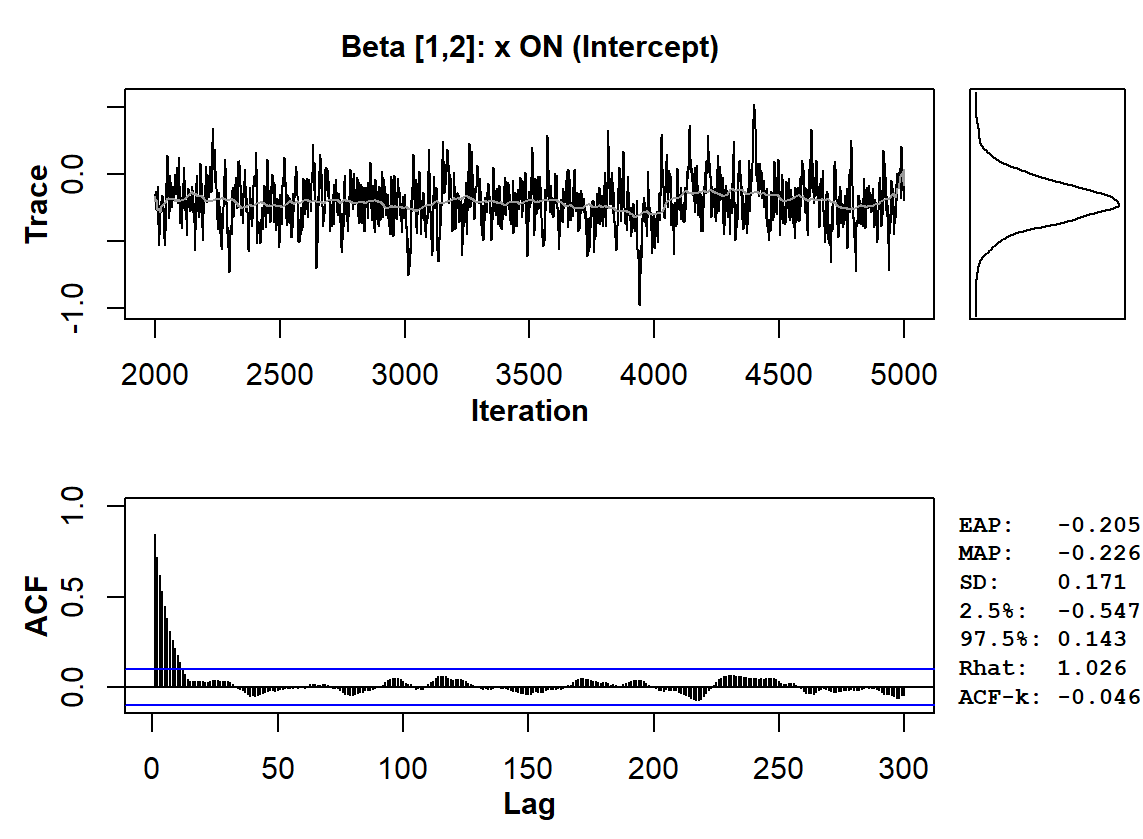
\includegraphics[width=0.65\linewidth,height=\textheight,keepaspectratio]{figures/beta12MI.png}

}

\caption{\label{fig-MIdiag1}Trace and autocorrelation plot in an
exemplary simulation run for the intercept in the imputation model for
\(X\) (multiple imputation).}

\end{figure}%

\begin{figure}

\centering{

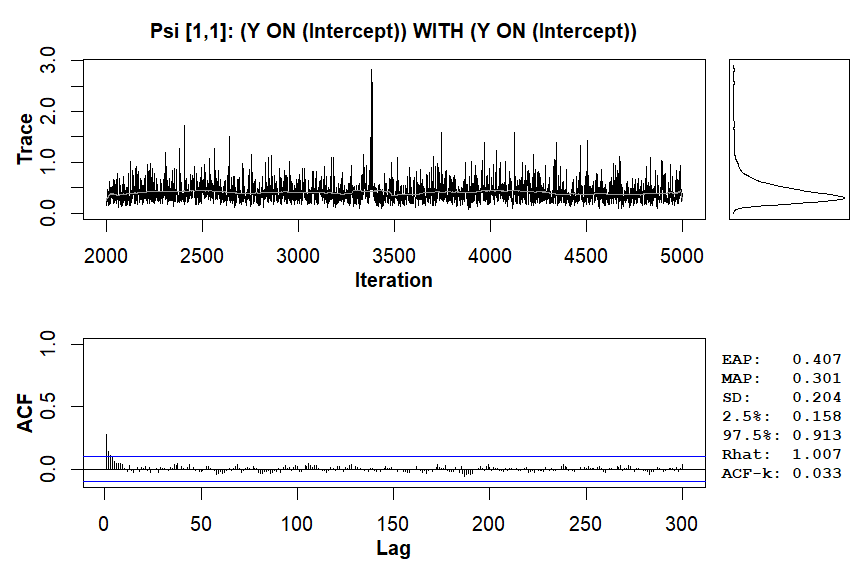
\includegraphics[width=0.65\linewidth,height=\textheight,keepaspectratio]{figures/psi11MI.png}

}

\caption{\label{fig-MIdiag2}Trace and autocorrelation plot in an
exemplary simulation run for the level-2 variance of \(Y\) (multiple
imputation).}

\end{figure}%

\begin{figure}

\centering{

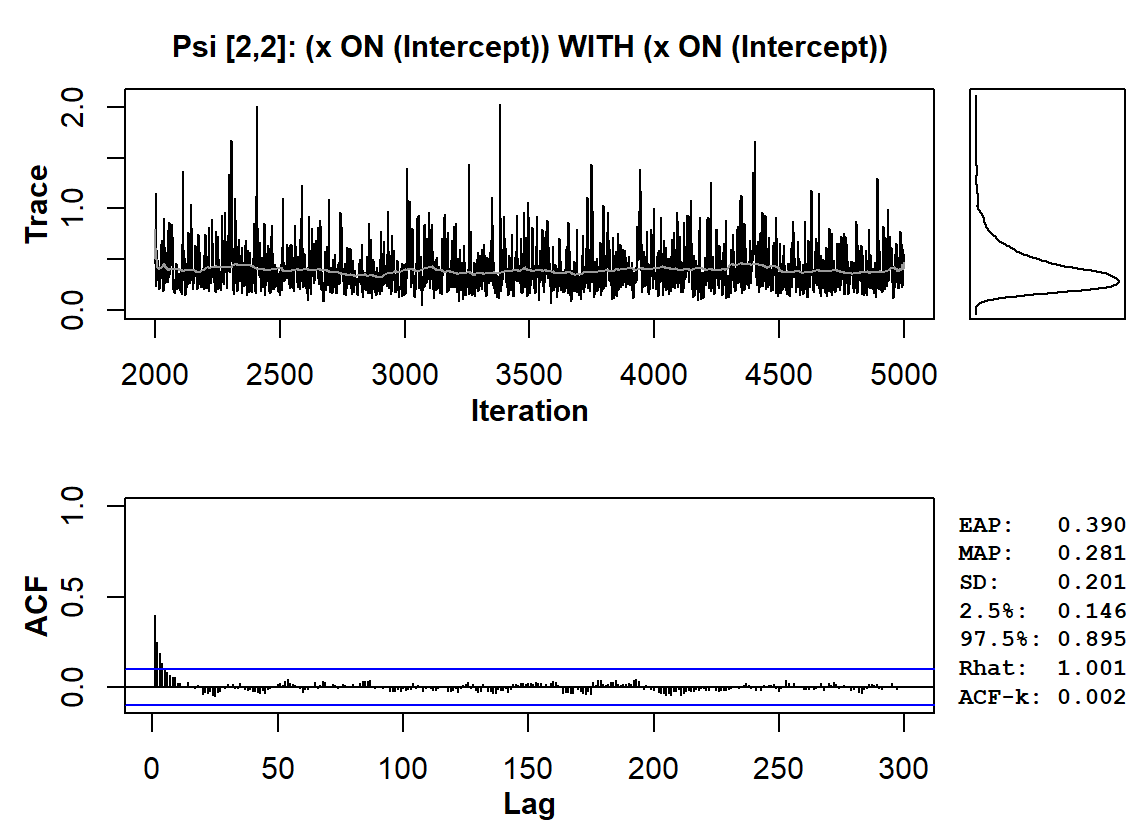
\includegraphics[width=0.65\linewidth,height=\textheight,keepaspectratio]{figures/psi22.png}

}

\caption{\label{fig-MIdiag3}Trace and autocorrelation plot in an
exemplary simulation run for the level-2 variance of \(X\) (multiple
imputation).}

\end{figure}%

\section{Diagnostics of fully Bayesian
analysis}\label{diagnostics-of-fully-bayesian-analysis}

\(\hat{R}\) values were close to 1, except for the level-2 variance of
\(X\) (\(\hat{R}=1.05\)) and the regression coefficient of the group
mean of \(X\) on \(W\) (\(\hat{R}=1.03\)). Diagnostic plots of these
parameters and the additionally critical parameter \(\tau_{y0}^2\) are
shown in Figure~\ref{fig-diagbayes}. Trace plots showed no drifting.
Autocorrelation decreased rapidly for most parameters, although some
exhibited persistent but low autocorrelation across lags. This pattern
suggests slightly reduced mixing efficiency rather than substantial
convergence problems (\citeproc{ref-johnson}{Johnson et al., 2022, pp.
149--152}).

\begin{figure}

\centering{

\includegraphics[width=0.7\linewidth,height=\textheight,keepaspectratio]{appendices/convergence_files/figure-pdf/fig-diagbayes-1.pdf}

}

\caption{\label{fig-diagbayes}Trace and autocorrelation plot for the
effect of the group mean of \(X\) on \(W\) in the imputation model
(fully Bayesian estimation).}

\end{figure}%

\begin{figure}

\centering{

\includegraphics[width=0.7\linewidth,height=\textheight,keepaspectratio]{appendices/convergence_files/figure-pdf/fig-plotbayes2-1.pdf}

}

\caption{\label{fig-plotbayes2}Trace and autocorrelation plot in an
exemplary simulation run for the level-2 variance of X (fully Bayesian
analysis)}

\end{figure}%

\begin{figure}

\centering{

\includegraphics[width=0.7\linewidth,height=\textheight,keepaspectratio]{appendices/convergence_files/figure-pdf/fig-plotbayes3-1.pdf}

}

\caption{\label{fig-plotbayes3}Trace and autocorrelation plot in an
exemplary simulation run for the level-2 variance of Y (fully Bayesian
analysis)}

\end{figure}%

\chapter{Complete simulation results}\label{sec-appB}

\begin{landscape}\begin{table}
\centering
\caption{\label{tab:unnamed-chunk-1}Simulation results ($N_2$ = 15, $\gamma_{01}$ = 0)}
\centering
\resizebox{\ifdim\width>\linewidth\linewidth\else\width\fi}{!}{
\begin{threeparttable}
\begin{tabular}[t]{lrrr>{}r|rrr>{}r|rrr>{}r|rrr>{}r|rrrr}
\toprule
\multicolumn{1}{c}{ } & \multicolumn{4}{c}{CD} & \multicolumn{4}{c}{LD} & \multicolumn{4}{c}{MI-R} & \multicolumn{4}{c}{MI-a} & \multicolumn{4}{c}{Bayes} \\
\cmidrule(l{3pt}r{3pt}){2-5} \cmidrule(l{3pt}r{3pt}){6-9} \cmidrule(l{3pt}r{3pt}){10-13} \cmidrule(l{3pt}r{3pt}){14-17} \cmidrule(l{3pt}r{3pt}){18-21}
Parameter & Bias & Cov & SD & CIW & Bias & Cov & SD & CIW & Bias & Cov & SD & CIW & Bias & Cov & SD & CIW & Bias & Cov & SD & CIW\\
\midrule
\addlinespace[0.3em]
\multicolumn{21}{c}{\textbf{MCAR}}\\
\addlinespace[0.3em]
\multicolumn{21}{l}{\textbf{ICC = 0.1}}\\
\hspace{1em}\hspace{1em}$\gamma_{01}$ & 0.002 & 0.942 & 0.284 & 1.170 & 0.037 & 0.941 & 0.300 & 1.180 & 0.005 & 0.966 & 0.252 & 1.115 & 0.005 & 0.986 & 0.252 & 1.284 & 0.003 & 0.980 & 0.291 & 1.456\\
\hspace{1em}\hspace{1em}$\gamma_{10}$ & -0.006 & 0.951 & 0.084 & 0.335 & -0.006 & 0.944 & 0.104 & 0.414 & -0.008 & 0.943 & 0.103 & 0.409 & -0.008 & 0.944 & 0.103 & 0.414 & -0.010 & 0.946 & 0.100 & 0.401\\
\addlinespace[0.3em]
\multicolumn{21}{l}{\textbf{ICC = 0.3}}\\
\hspace{1em}\hspace{1em}$\gamma_{01}$ & 0.000 & 0.960 & 0.272 & 1.174 & 0.012 & 0.953 & 0.280 & 1.177 & -0.001 & 0.942 & 0.278 & 1.126 & -0.001 & 0.972 & 0.278 & 1.278 & -0.003 & 0.980 & 0.288 & 1.384\\
\hspace{1em}\hspace{1em}$\gamma_{10}$ & 0.001 & 0.942 & 0.089 & 0.336 & 0.000 & 0.931 & 0.111 & 0.415 & -0.005 & 0.938 & 0.108 & 0.411 & -0.005 & 0.939 & 0.108 & 0.416 & -0.006 & 0.934 & 0.108 & 0.405\\
\addlinespace[0.3em]
\multicolumn{21}{c}{\textbf{MAR}}\\
\addlinespace[0.3em]
\multicolumn{21}{l}{\textbf{ICC = 0.1}}\\
\hspace{1em}\hspace{1em}$\gamma_{01}$ & -0.002 & 0.949 & 0.283 & 1.192 & 0.031 & 0.947 & 0.284 & 1.189 & 0.007 & 0.970 & 0.247 & 1.131 & 0.007 & 0.985 & 0.247 & 1.305 & 0.001 & 0.987 & 0.289 & 1.481\\
\hspace{1em}\hspace{1em}$\gamma_{10}$ & 0.000 & 0.942 & 0.087 & 0.336 & -0.002 & 0.954 & 0.106 & 0.416 & -0.007 & 0.949 & 0.104 & 0.412 & -0.007 & 0.950 & 0.104 & 0.418 & -0.007 & 0.954 & 0.102 & 0.403\\
\addlinespace[0.3em]
\multicolumn{21}{l}{\textbf{ICC = 0.3}}\\
\hspace{1em}\hspace{1em}$\gamma_{01}$ & -0.016 & 0.943 & 0.279 & 1.175 & 0.007 & 0.949 & 0.279 & 1.175 & -0.014 & 0.943 & 0.275 & 1.130 & -0.014 & 0.968 & 0.275 & 1.285 & -0.016 & 0.975 & 0.291 & 1.390\\
\hspace{1em}\hspace{1em}$\gamma_{10}$ & 0.001 & 0.941 & 0.087 & 0.337 & -0.001 & 0.948 & 0.105 & 0.414 & -0.004 & 0.943 & 0.102 & 0.411 & -0.004 & 0.945 & 0.102 & 0.417 & -0.005 & 0.949 & 0.101 & 0.405\\
\bottomrule
\end{tabular}
\begin{tablenotes}
\item \textit{Note: } 
\item Bias = average deviation from the true parameter;  Cov = empirical coverage rate;  SD = empirical standard deviation;  CIW = mean confidence/credible interval width.  MCAR = missing completely at random; MAR = missing at random.  CD = complete data; LD = listwise deletion;  MI-R = multiple imputation using Rubin's degrees-of-freedom approximation;  MI-a = multiple imputation using small-sample-adjusted degrees of freedom;  Bayes = fully Bayesian estimation.
\end{tablenotes}
\end{threeparttable}}
\end{table}
\end{landscape}

\begin{landscape}\begin{table}
\centering
\caption{\label{tab:unnamed-chunk-2}Simulation results ($N_2$ = 15, $\gamma_{01}$ = 0.4)}
\centering
\resizebox{\ifdim\width>\linewidth\linewidth\else\width\fi}{!}{
\begin{threeparttable}
\begin{tabular}[t]{lrrr>{}r|rrr>{}r|rrr>{}r|rrr>{}r|rrrr}
\toprule
\multicolumn{1}{c}{ } & \multicolumn{4}{c}{CD} & \multicolumn{4}{c}{LD} & \multicolumn{4}{c}{MI-R} & \multicolumn{4}{c}{MI-a} & \multicolumn{4}{c}{Bayes} \\
\cmidrule(l{3pt}r{3pt}){2-5} \cmidrule(l{3pt}r{3pt}){6-9} \cmidrule(l{3pt}r{3pt}){10-13} \cmidrule(l{3pt}r{3pt}){14-17} \cmidrule(l{3pt}r{3pt}){18-21}
 & Bias & Cov & SD & CIW & Bias & Cov & SD & CIW & Bias & Cov & SD & CIW & Bias & Cov & SD & CIW & Bias & Cov & SD & CIW\\
\midrule
\addlinespace[0.3em]
\multicolumn{21}{c}{\textbf{MCAR}}\\
\addlinespace[0.3em]
\multicolumn{21}{l}{\textbf{ICC = .1}}\\
\hspace{1em}\hspace{1em}$\gamma_{01}$ & -0.008 & 0.953 & 0.275 & 1.174 & -0.038 & 0.968 & 0.269 & 1.183 & -0.075 & 0.965 & 0.239 & 1.151 & -0.075 & 0.981 & 0.239 & 1.329 & -0.036 & 0.985 & 0.281 & 1.516\\
\hspace{1em}\hspace{1em}$\gamma_{10}$ & 0.000 & 0.952 & 0.083 & 0.330 & 0.000 & 0.952 & 0.102 & 0.404 & -0.001 & 0.950 & 0.101 & 0.401 & -0.001 & 0.953 & 0.101 & 0.407 & -0.003 & 0.954 & 0.099 & 0.393\\
\addlinespace[0.3em]
\multicolumn{21}{l}{\textbf{ICC = .3}}\\
\hspace{1em}\hspace{1em}$\gamma_{01}$ & 0.003 & 0.955 & 0.272 & 1.154 & -0.013 & 0.949 & 0.272 & 1.156 & -0.016 & 0.951 & 0.275 & 1.122 & -0.016 & 0.967 & 0.275 & 1.277 & -0.008 & 0.971 & 0.290 & 1.385\\
\hspace{1em}\hspace{1em}$\gamma_{10}$ & 0.002 & 0.949 & 0.083 & 0.326 & 0.003 & 0.935 & 0.106 & 0.402 & -0.001 & 0.944 & 0.103 & 0.397 & -0.001 & 0.948 & 0.103 & 0.402 & -0.003 & 0.942 & 0.101 & 0.391\\
\addlinespace[0.3em]
\multicolumn{21}{c}{\textbf{MAR}}\\
\addlinespace[0.3em]
\multicolumn{21}{l}{\textbf{ICC = .1}}\\
\hspace{1em}\hspace{1em}$\gamma_{01}$ & -0.004 & 0.959 & 0.276 & 1.151 & -0.050 & 0.942 & 0.283 & 1.169 & -0.078 & 0.965 & 0.238 & 1.124 & -0.078 & 0.977 & 0.238 & 1.299 & -0.039 & 0.982 & 0.276 & 1.461\\
\hspace{1em}\hspace{1em}$\gamma_{10}$ & -0.007 & 0.954 & 0.084 & 0.331 & -0.005 & 0.952 & 0.105 & 0.408 & -0.007 & 0.956 & 0.102 & 0.404 & -0.007 & 0.959 & 0.102 & 0.409 & -0.010 & 0.952 & 0.101 & 0.396\\
\addlinespace[0.3em]
\multicolumn{21}{l}{\textbf{ICC = .3}}\\
\hspace{1em}\hspace{1em}$\gamma_{01}$ & 0.006 & 0.962 & 0.269 & 1.162 & -0.019 & 0.956 & 0.275 & 1.165 & -0.020 & 0.947 & 0.271 & 1.137 & -0.020 & 0.976 & 0.271 & 1.296 & -0.008 & 0.977 & 0.290 & 1.407\\
\hspace{1em}\hspace{1em}$\gamma_{10}$ & -0.001 & 0.945 & 0.086 & 0.327 & 0.000 & 0.948 & 0.105 & 0.403 & -0.003 & 0.946 & 0.102 & 0.398 & -0.003 & 0.948 & 0.102 & 0.403 & -0.006 & 0.951 & 0.102 & 0.393\\
\bottomrule
\end{tabular}
\begin{tablenotes}
\item \textit{Note: } 
\item Abbreviations as listed in Table C.1
\end{tablenotes}
\end{threeparttable}}
\end{table}
\end{landscape}

\begin{landscape}\begin{table}
\centering
\caption{\label{tab:unnamed-chunk-3}Simulation results ($N_2$ = 30, $\gamma_{01}$ = 0)}
\centering
\resizebox{\ifdim\width>\linewidth\linewidth\else\width\fi}{!}{
\begin{threeparttable}
\begin{tabular}[t]{lrrr>{}r|rrr>{}r|rrr>{}r|rrr>{}r|rrrr}
\toprule
\multicolumn{1}{c}{ } & \multicolumn{4}{c}{CD} & \multicolumn{4}{c}{LD} & \multicolumn{4}{c}{MI-R} & \multicolumn{4}{c}{MI-a} & \multicolumn{4}{c}{Bayes} \\
\cmidrule(l{3pt}r{3pt}){2-5} \cmidrule(l{3pt}r{3pt}){6-9} \cmidrule(l{3pt}r{3pt}){10-13} \cmidrule(l{3pt}r{3pt}){14-17} \cmidrule(l{3pt}r{3pt}){18-21}
 & Bias & Cov & SD & CIW & Bias & Cov & SD & CIW & Bias & Cov & SD & CIW & Bias & Cov & SD & CIW & Bias & Cov & SD & CIW\\
\midrule
\addlinespace[0.3em]
\multicolumn{21}{c}{\textbf{MCAR}}\\
\addlinespace[0.3em]
\multicolumn{21}{l}{\textbf{ICC = .1}}\\
\hspace{1em}\hspace{1em}$\gamma_{01}$ & 0.003 & 0.945 & 0.188 & 0.755 & 0.042 & 0.939 & 0.186 & 0.757 & 0.014 & 0.962 & 0.173 & 0.766 & 0.014 & 0.976 & 0.173 & 0.812 & 0.009 & 0.963 & 0.199 & 0.864\\
\hspace{1em}\hspace{1em}$\gamma_{10}$ & -0.005 & 0.953 & 0.059 & 0.236 & -0.006 & 0.953 & 0.073 & 0.291 & -0.007 & 0.954 & 0.073 & 0.290 & -0.007 & 0.954 & 0.073 & 0.292 & -0.008 & 0.950 & 0.072 & 0.283\\
\addlinespace[0.3em]
\multicolumn{21}{l}{\textbf{ICC = .3}}\\
\hspace{1em}\hspace{1em}$\gamma_{01}$ & -0.004 & 0.957 & 0.185 & 0.758 & 0.010 & 0.964 & 0.185 & 0.760 & -0.003 & 0.955 & 0.190 & 0.769 & -0.003 & 0.964 & 0.190 & 0.810 & -0.003 & 0.965 & 0.192 & 0.826\\
\hspace{1em}\hspace{1em}$\gamma_{10}$ & 0.001 & 0.942 & 0.063 & 0.237 & 0.000 & 0.943 & 0.077 & 0.291 & -0.003 & 0.939 & 0.077 & 0.291 & -0.003 & 0.940 & 0.077 & 0.293 & -0.003 & 0.943 & 0.076 & 0.284\\
\addlinespace[0.3em]
\multicolumn{21}{c}{\textbf{MAR}}\\
\addlinespace[0.3em]
\multicolumn{21}{l}{\textbf{ICC = .1}}\\
\hspace{1em}\hspace{1em}$\gamma_{01}$ & 0.006 & 0.941 & 0.191 & 0.757 & 0.039 & 0.947 & 0.192 & 0.761 & 0.010 & 0.965 & 0.177 & 0.767 & 0.010 & 0.972 & 0.177 & 0.813 & 0.003 & 0.965 & 0.203 & 0.870\\
\hspace{1em}\hspace{1em}$\gamma_{10}$ & 0.000 & 0.944 & 0.061 & 0.236 & -0.002 & 0.945 & 0.075 & 0.290 & -0.003 & 0.950 & 0.074 & 0.288 & -0.003 & 0.951 & 0.074 & 0.290 & -0.004 & 0.948 & 0.073 & 0.282\\
\addlinespace[0.3em]
\multicolumn{21}{l}{\textbf{ICC = .3}}\\
\hspace{1em}\hspace{1em}$\gamma_{01}$ & 0.008 & 0.969 & 0.179 & 0.765 & 0.027 & 0.956 & 0.183 & 0.768 & 0.011 & 0.958 & 0.186 & 0.777 & 0.011 & 0.968 & 0.186 & 0.820 & 0.010 & 0.967 & 0.188 & 0.836\\
\hspace{1em}\hspace{1em}$\gamma_{10}$ & 0.000 & 0.944 & 0.062 & 0.238 & 0.000 & 0.948 & 0.076 & 0.293 & -0.003 & 0.954 & 0.075 & 0.294 & -0.003 & 0.954 & 0.075 & 0.296 & -0.003 & 0.946 & 0.074 & 0.286\\
\bottomrule
\end{tabular}
\begin{tablenotes}
\item \textit{Note: } 
\item Abbreviations as listed in Table C.1
\end{tablenotes}
\end{threeparttable}}
\end{table}
\end{landscape}

\begin{landscape}\begin{table}
\centering
\caption{\label{tab:unnamed-chunk-4}Simulation results ($N_2$ = 30, $\gamma_{01}$ = 0.4)}
\centering
\resizebox{\ifdim\width>\linewidth\linewidth\else\width\fi}{!}{
\begin{threeparttable}
\begin{tabular}[t]{lrrr>{}r|rrr>{}r|rrr>{}r|rrr>{}r|rrrr}
\toprule
\multicolumn{1}{c}{ } & \multicolumn{4}{c}{CD} & \multicolumn{4}{c}{LD} & \multicolumn{4}{c}{MI-R} & \multicolumn{4}{c}{MI-a} & \multicolumn{4}{c}{Bayes} \\
\cmidrule(l{3pt}r{3pt}){2-5} \cmidrule(l{3pt}r{3pt}){6-9} \cmidrule(l{3pt}r{3pt}){10-13} \cmidrule(l{3pt}r{3pt}){14-17} \cmidrule(l{3pt}r{3pt}){18-21}
 & Bias & Cov & SD & CIW & Bias & Cov & SD & CIW & Bias & Cov & SD & CIW & Bias & Cov & SD & CIW & Bias & Cov & SD & CIW\\
\midrule
\addlinespace[0.3em]
\multicolumn{21}{c}{\textbf{MCAR}}\\
\addlinespace[0.3em]
\multicolumn{21}{l}{\textbf{ICC = .1}}\\
\hspace{1em}\hspace{1em}$\gamma_{01}$ & 0.005 & 0.950 & 0.189 & 0.744 & -0.034 & 0.956 & 0.187 & 0.748 & -0.052 & 0.956 & 0.175 & 0.767 & -0.052 & 0.966 & 0.175 & 0.813 & -0.009 & 0.970 & 0.204 & 0.865\\
\hspace{1em}\hspace{1em}$\gamma_{10}$ & 0.000 & 0.966 & 0.056 & 0.231 & -0.001 & 0.967 & 0.068 & 0.284 & 0.001 & 0.966 & 0.066 & 0.283 & 0.001 & 0.969 & 0.066 & 0.285 & -0.003 & 0.967 & 0.065 & 0.277\\
\addlinespace[0.3em]
\multicolumn{21}{l}{\textbf{ICC = .3}}\\
\hspace{1em}\hspace{1em}$\gamma_{01}$ & 0.007 & 0.943 & 0.188 & 0.736 & -0.008 & 0.941 & 0.191 & 0.740 & -0.002 & 0.938 & 0.194 & 0.753 & -0.002 & 0.953 & 0.194 & 0.794 & 0.004 & 0.951 & 0.201 & 0.811\\
\hspace{1em}\hspace{1em}$\gamma_{10}$ & 0.000 & 0.963 & 0.057 & 0.229 & 0.003 & 0.956 & 0.069 & 0.282 & 0.001 & 0.950 & 0.067 & 0.281 & 0.001 & 0.954 & 0.067 & 0.283 & 0.000 & 0.954 & 0.067 & 0.275\\
\addlinespace[0.3em]
\multicolumn{21}{c}{\textbf{MAR}}\\
\addlinespace[0.3em]
\multicolumn{21}{l}{\textbf{ICC = .1}}\\
\hspace{1em}\hspace{1em}$\gamma_{01}$ & 0.005 & 0.948 & 0.191 & 0.744 & -0.033 & 0.944 & 0.190 & 0.749 & -0.057 & 0.952 & 0.174 & 0.772 & -0.057 & 0.963 & 0.174 & 0.819 & -0.015 & 0.958 & 0.204 & 0.868\\
\hspace{1em}\hspace{1em}$\gamma_{10}$ & 0.001 & 0.947 & 0.060 & 0.233 & 0.001 & 0.946 & 0.073 & 0.285 & 0.003 & 0.948 & 0.073 & 0.285 & 0.003 & 0.950 & 0.073 & 0.287 & 0.000 & 0.946 & 0.071 & 0.277\\
\addlinespace[0.3em]
\multicolumn{21}{l}{\textbf{ICC = .3}}\\
\hspace{1em}\hspace{1em}$\gamma_{01}$ & 0.002 & 0.941 & 0.182 & 0.737 & -0.014 & 0.947 & 0.180 & 0.738 & -0.006 & 0.942 & 0.185 & 0.754 & -0.006 & 0.951 & 0.185 & 0.795 & 0.000 & 0.954 & 0.191 & 0.813\\
\hspace{1em}\hspace{1em}$\gamma_{10}$ & -0.002 & 0.948 & 0.059 & 0.230 & -0.001 & 0.947 & 0.075 & 0.284 & -0.003 & 0.950 & 0.072 & 0.283 & -0.003 & 0.951 & 0.072 & 0.285 & -0.004 & 0.948 & 0.072 & 0.277\\
\bottomrule
\end{tabular}
\begin{tablenotes}
\item \textit{Note: } 
\item Abbreviations as listed in Table C.1
\end{tablenotes}
\end{threeparttable}}
\end{table}
\end{landscape}

\begin{landscape}\begin{table}
\centering
\caption{\label{tab:unnamed-chunk-5}Simulation results ($N_2$ = 60, $\gamma_{01}$ = 0)}
\centering
\resizebox{\ifdim\width>\linewidth\linewidth\else\width\fi}{!}{
\begin{threeparttable}
\begin{tabular}[t]{lrrr>{}r|rrr>{}r|rrr>{}r|rrr>{}r|rrrr}
\toprule
\multicolumn{1}{c}{ } & \multicolumn{4}{c}{CD} & \multicolumn{4}{c}{LD} & \multicolumn{4}{c}{MI-R} & \multicolumn{4}{c}{MI-a} & \multicolumn{4}{c}{Bayes} \\
\cmidrule(l{3pt}r{3pt}){2-5} \cmidrule(l{3pt}r{3pt}){6-9} \cmidrule(l{3pt}r{3pt}){10-13} \cmidrule(l{3pt}r{3pt}){14-17} \cmidrule(l{3pt}r{3pt}){18-21}
 & Bias & Cov & SD & CIW & Bias & Cov & SD & CIW & Bias & Cov & SD & CIW & Bias & Cov & SD & CIW & Bias & Cov & SD & CIW\\
\midrule
\addlinespace[0.3em]
\multicolumn{21}{c}{\textbf{MCAR}}\\
\addlinespace[0.3em]
\multicolumn{21}{l}{\textbf{ICC = .1}}\\
\hspace{1em}\hspace{1em}$\gamma_{01}$ & -0.006 & 0.955 & 0.130 & 0.516 & 0.027 & 0.954 & 0.128 & 0.517 & -0.002 & 0.971 & 0.124 & 0.542 & -0.002 & 0.979 & 0.124 & 0.556 & -0.010 & 0.961 & 0.139 & 0.575\\
\hspace{1em}\hspace{1em}$\gamma_{10}$ & 0.000 & 0.944 & 0.043 & 0.167 & -0.001 & 0.953 & 0.053 & 0.205 & -0.002 & 0.939 & 0.053 & 0.205 & -0.002 & 0.940 & 0.053 & 0.206 & -0.002 & 0.945 & 0.052 & 0.199\\
\addlinespace[0.3em]
\multicolumn{21}{l}{\textbf{ICC = .3}}\\
\hspace{1em}\hspace{1em}$\gamma_{01}$ & -0.002 & 0.946 & 0.127 & 0.518 & 0.017 & 0.955 & 0.127 & 0.519 & 0.001 & 0.949 & 0.132 & 0.536 & 0.001 & 0.954 & 0.132 & 0.549 & 0.000 & 0.954 & 0.133 & 0.550\\
\hspace{1em}\hspace{1em}$\gamma_{10}$ & 0.000 & 0.947 & 0.042 & 0.167 & 0.002 & 0.947 & 0.052 & 0.206 & 0.000 & 0.948 & 0.051 & 0.206 & 0.000 & 0.948 & 0.051 & 0.206 & 0.000 & 0.946 & 0.051 & 0.201\\
\addlinespace[0.3em]
\multicolumn{21}{c}{\textbf{MAR}}\\
\addlinespace[0.3em]
\multicolumn{21}{l}{\textbf{ICC = .1}}\\
\hspace{1em}\hspace{1em}$\gamma_{01}$ & 0.000 & 0.951 & 0.131 & 0.517 & 0.037 & 0.949 & 0.129 & 0.520 & 0.008 & 0.960 & 0.126 & 0.545 & 0.008 & 0.965 & 0.126 & 0.559 & 0.001 & 0.953 & 0.142 & 0.582\\
\hspace{1em}\hspace{1em}$\gamma_{10}$ & -0.001 & 0.954 & 0.043 & 0.167 & 0.000 & 0.954 & 0.052 & 0.204 & -0.001 & 0.956 & 0.051 & 0.205 & -0.001 & 0.957 & 0.051 & 0.205 & -0.001 & 0.953 & 0.050 & 0.198\\
\addlinespace[0.3em]
\multicolumn{21}{l}{\textbf{ICC = .3}}\\
\hspace{1em}\hspace{1em}$\gamma_{01}$ & 0.005 & 0.948 & 0.131 & 0.522 & 0.021 & 0.949 & 0.131 & 0.522 & 0.003 & 0.946 & 0.137 & 0.539 & 0.003 & 0.949 & 0.137 & 0.552 & 0.003 & 0.956 & 0.137 & 0.556\\
\hspace{1em}\hspace{1em}$\gamma_{10}$ & 0.001 & 0.954 & 0.041 & 0.167 & 0.000 & 0.949 & 0.052 & 0.205 & -0.001 & 0.947 & 0.052 & 0.205 & -0.001 & 0.947 & 0.052 & 0.206 & -0.001 & 0.944 & 0.051 & 0.201\\
\bottomrule
\end{tabular}
\begin{tablenotes}
\item \textit{Note: } 
\item Abbreviations as listed in Table C.1
\end{tablenotes}
\end{threeparttable}}
\end{table}
\end{landscape}

\begin{landscape}\begin{table}
\centering
\caption{\label{tab:unnamed-chunk-6}Simulation results ($N_2$ = 60, $\gamma_{01}$ = 0.4)}
\centering
\resizebox{\ifdim\width>\linewidth\linewidth\else\width\fi}{!}{
\begin{threeparttable}
\begin{tabular}[t]{lrrr>{}r|rrr>{}r|rrr>{}r|rrr>{}r|rrrr}
\toprule
\multicolumn{1}{c}{ } & \multicolumn{4}{c}{CD} & \multicolumn{4}{c}{LD} & \multicolumn{4}{c}{MI-R} & \multicolumn{4}{c}{MI-a} & \multicolumn{4}{c}{Bayes} \\
\cmidrule(l{3pt}r{3pt}){2-5} \cmidrule(l{3pt}r{3pt}){6-9} \cmidrule(l{3pt}r{3pt}){10-13} \cmidrule(l{3pt}r{3pt}){14-17} \cmidrule(l{3pt}r{3pt}){18-21}
 & Bias & Cov & SD & CIW & Bias & Cov & SD & CIW & Bias & Cov & SD & CIW & Bias & Cov & SD & CIW & Bias & Cov & SD & CIW\\
\midrule
\addlinespace[0.3em]
\multicolumn{21}{c}{\textbf{MCAR}}\\
\addlinespace[0.3em]
\multicolumn{21}{l}{\textbf{ICC = .1}}\\
\hspace{1em}\hspace{1em}$\gamma_{01}$ & 0.001 & 0.946 & 0.126 & 0.509 & -0.039 & 0.939 & 0.124 & 0.509 & -0.044 & 0.955 & 0.121 & 0.541 & -0.044 & 0.960 & 0.121 & 0.556 & -0.008 & 0.952 & 0.136 & 0.577\\
\hspace{1em}\hspace{1em}$\gamma_{10}$ & 0.001 & 0.960 & 0.041 & 0.164 & 0.001 & 0.961 & 0.050 & 0.201 & 0.004 & 0.954 & 0.049 & 0.200 & 0.004 & 0.955 & 0.049 & 0.200 & 0.001 & 0.958 & 0.049 & 0.195\\
\addlinespace[0.3em]
\multicolumn{21}{l}{\textbf{ICC = .3}}\\
\hspace{1em}\hspace{1em}$\gamma_{01}$ & -0.002 & 0.952 & 0.129 & 0.501 & -0.021 & 0.947 & 0.128 & 0.502 & -0.007 & 0.954 & 0.132 & 0.521 & -0.007 & 0.957 & 0.132 & 0.534 & -0.005 & 0.962 & 0.133 & 0.536\\
\hspace{1em}\hspace{1em}$\gamma_{10}$ & -0.001 & 0.954 & 0.040 & 0.162 & -0.001 & 0.956 & 0.049 & 0.199 & -0.002 & 0.956 & 0.048 & 0.199 & -0.002 & 0.956 & 0.048 & 0.200 & -0.002 & 0.961 & 0.048 & 0.194\\
\addlinespace[0.3em]
\multicolumn{21}{c}{\textbf{MAR}}\\
\addlinespace[0.3em]
\multicolumn{21}{l}{\textbf{ICC = .1}}\\
\hspace{1em}\hspace{1em}$\gamma_{01}$ & 0.000 & 0.954 & 0.129 & 0.509 & -0.035 & 0.943 & 0.128 & 0.512 & -0.044 & 0.960 & 0.125 & 0.544 & -0.044 & 0.962 & 0.125 & 0.559 & -0.008 & 0.957 & 0.144 & 0.580\\
\hspace{1em}\hspace{1em}$\gamma_{10}$ & 0.002 & 0.926 & 0.043 & 0.163 & 0.001 & 0.942 & 0.051 & 0.200 & 0.003 & 0.941 & 0.050 & 0.199 & 0.003 & 0.942 & 0.050 & 0.200 & 0.001 & 0.941 & 0.050 & 0.194\\
\addlinespace[0.3em]
\multicolumn{21}{l}{\textbf{ICC = .3}}\\
\hspace{1em}\hspace{1em}$\gamma_{01}$ & -0.005 & 0.950 & 0.127 & 0.503 & -0.022 & 0.956 & 0.125 & 0.504 & -0.009 & 0.958 & 0.130 & 0.523 & -0.009 & 0.961 & 0.130 & 0.536 & -0.008 & 0.962 & 0.132 & 0.540\\
\hspace{1em}\hspace{1em}$\gamma_{10}$ & -0.001 & 0.953 & 0.042 & 0.162 & -0.002 & 0.944 & 0.051 & 0.199 & -0.003 & 0.944 & 0.050 & 0.199 & -0.003 & 0.945 & 0.050 & 0.200 & -0.003 & 0.942 & 0.050 & 0.195\\
\bottomrule
\end{tabular}
\begin{tablenotes}
\item \textit{Note: } 
\item Abbreviations as listed in Table C.1
\end{tablenotes}
\end{threeparttable}}
\end{table}
\end{landscape}

\begin{landscape}\begin{table}
\centering
\caption{\label{tab:unnamed-chunk-7}MCSEs of performance measures ($N_2$ = 15, $\gamma_{01}$ = 0)}
\centering
\resizebox{\ifdim\width>\linewidth\linewidth\else\width\fi}{!}{
\begin{threeparttable}
\begin{tabular}[t]{lrrr>{}r|rrr>{}r|rrr>{}r|rrr>{}r|rrrr}
\toprule
\multicolumn{1}{c}{ } & \multicolumn{4}{c}{CD} & \multicolumn{4}{c}{LD} & \multicolumn{4}{c}{MI-R} & \multicolumn{4}{c}{MI-a} & \multicolumn{4}{c}{Bayes} \\
\cmidrule(l{3pt}r{3pt}){2-5} \cmidrule(l{3pt}r{3pt}){6-9} \cmidrule(l{3pt}r{3pt}){10-13} \cmidrule(l{3pt}r{3pt}){14-17} \cmidrule(l{3pt}r{3pt}){18-21}
 & Bias & Cov & SD & CIW & Bias & Cov & SD & CIW & Bias & Cov & SD & CIW & Bias & Cov & SD & CIW & Bias & Cov & SD & CIW\\
\midrule
\addlinespace[0.3em]
\multicolumn{21}{c}{\textbf{MCAR}}\\
\addlinespace[0.3em]
\multicolumn{21}{l}{\textbf{ICC = .1}}\\
\hspace{1em}\hspace{1em}$\gamma_{01}$ & 0.009 & 0.007 & 0.006 & 0.010 & 0.009 & 0.007 & 0.007 & 0.010 & 0.008 & 0.006 & 0.006 & 0.010 & 0.008 & 0.004 & 0.006 & 0.012 & 0.009 & 0.004 & 0.007 & 0.014\\
\hspace{1em}\hspace{1em}$\gamma_{10}$ & 0.003 & 0.007 & 0.002 & 0.001 & 0.003 & 0.007 & 0.002 & 0.001 & 0.003 & 0.007 & 0.002 & 0.002 & 0.003 & 0.007 & 0.002 & 0.002 & 0.003 & 0.007 & 0.002 & \vphantom{2} 0.001\\
\addlinespace[0.3em]
\multicolumn{21}{l}{\textbf{ICC = .3}}\\
\hspace{1em}\hspace{1em}$\gamma_{01}$ & 0.009 & 0.006 & 0.006 & 0.010 & 0.009 & 0.007 & 0.006 & 0.010 & 0.009 & 0.007 & 0.006 & 0.011 & 0.009 & 0.005 & 0.006 & 0.012 & 0.009 & 0.004 & 0.006 & 0.013\\
\hspace{1em}\hspace{1em}$\gamma_{10}$ & 0.003 & 0.007 & 0.002 & 0.001 & 0.004 & 0.008 & 0.002 & 0.001 & 0.003 & 0.008 & 0.002 & 0.002 & 0.003 & 0.008 & 0.002 & 0.002 & 0.003 & 0.008 & 0.002 & 0.001\\
\addlinespace[0.3em]
\multicolumn{21}{c}{\textbf{MAR}}\\
\addlinespace[0.3em]
\multicolumn{21}{l}{\textbf{ICC = .1}}\\
\hspace{1em}\hspace{1em}$\gamma_{01}$ & 0.009 & 0.007 & 0.006 & 0.011 & 0.009 & 0.007 & 0.006 & 0.011 & 0.008 & 0.005 & 0.006 & 0.011 & 0.008 & 0.004 & 0.006 & 0.013 & 0.009 & 0.004 & 0.006 & 0.016\\
\hspace{1em}\hspace{1em}$\gamma_{10}$ & 0.003 & 0.007 & 0.002 & 0.001 & 0.003 & 0.007 & 0.002 & 0.001 & 0.003 & 0.007 & 0.002 & 0.002 & 0.003 & 0.007 & 0.002 & 0.002 & 0.003 & 0.007 & 0.002 & \vphantom{1} 0.001\\
\addlinespace[0.3em]
\multicolumn{21}{l}{\textbf{ICC = .3}}\\
\hspace{1em}\hspace{1em}$\gamma_{01}$ & 0.009 & 0.007 & 0.006 & 0.011 & 0.009 & 0.007 & 0.006 & 0.011 & 0.009 & 0.007 & 0.006 & 0.011 & 0.009 & 0.006 & 0.006 & 0.013 & 0.009 & 0.005 & 0.007 & 0.014\\
\hspace{1em}\hspace{1em}$\gamma_{10}$ & 0.003 & 0.007 & 0.002 & 0.001 & 0.003 & 0.007 & 0.002 & 0.001 & 0.003 & 0.007 & 0.002 & 0.002 & 0.003 & 0.007 & 0.002 & 0.002 & 0.003 & 0.007 & 0.002 & 0.001\\
\bottomrule
\end{tabular}
\begin{tablenotes}
\item \textit{Note: } 
\item All entries are Monte Carlo standard errors (MCSEs).  Abbreviations as listed in Table C.1.
\end{tablenotes}
\end{threeparttable}}
\end{table}
\end{landscape}

\begin{landscape}\begin{table}
\centering
\caption{\label{tab:unnamed-chunk-8}MCSEs of performance measures ($N_2$ = 15, $\gamma_{01}$ = 0.4)}
\centering
\resizebox{\ifdim\width>\linewidth\linewidth\else\width\fi}{!}{
\begin{threeparttable}
\begin{tabular}[t]{lrrr>{}r|rrr>{}r|rrr>{}r|rrr>{}r|rrrr}
\toprule
\multicolumn{1}{c}{ } & \multicolumn{4}{c}{CD} & \multicolumn{4}{c}{LD} & \multicolumn{4}{c}{MI-R} & \multicolumn{4}{c}{MI-a} & \multicolumn{4}{c}{Bayes} \\
\cmidrule(l{3pt}r{3pt}){2-5} \cmidrule(l{3pt}r{3pt}){6-9} \cmidrule(l{3pt}r{3pt}){10-13} \cmidrule(l{3pt}r{3pt}){14-17} \cmidrule(l{3pt}r{3pt}){18-21}
 & Bias & Cov & SD & CIW & Bias & Cov & SD & CIW & Bias & Cov & SD & CIW & Bias & Cov & SD & CIW & Bias & Cov & SD & CIW\\
\midrule
\addlinespace[0.3em]
\multicolumn{21}{c}{\textbf{MCAR}}\\
\addlinespace[0.3em]
\multicolumn{21}{l}{\textbf{ICC = .1}}\\
\hspace{1em}\hspace{1em}$\gamma_{01}$ & 0.009 & 0.007 & 0.006 & 0.010 & 0.008 & 0.006 & 0.006 & 0.010 & 0.008 & 0.006 & 0.005 & 0.010 & 0.008 & 0.004 & 0.005 & 0.013 & 0.009 & 0.004 & 0.006 & 0.020\\
\hspace{1em}\hspace{1em}$\gamma_{10}$ & 0.003 & 0.007 & 0.002 & 0.001 & 0.003 & 0.007 & 0.002 & 0.001 & 0.003 & 0.007 & 0.002 & 0.002 & 0.003 & 0.007 & 0.002 & 0.002 & 0.003 & 0.007 & 0.002 & \vphantom{1} 0.001\\
\addlinespace[0.3em]
\multicolumn{21}{l}{\textbf{ICC = .3}}\\
\hspace{1em}\hspace{1em}$\gamma_{01}$ & 0.009 & 0.007 & 0.006 & 0.011 & 0.009 & 0.007 & 0.006 & 0.011 & 0.009 & 0.007 & 0.006 & 0.011 & 0.009 & 0.006 & 0.006 & 0.013 & 0.009 & 0.005 & 0.006 & 0.016\\
\hspace{1em}\hspace{1em}$\gamma_{10}$ & 0.003 & 0.007 & 0.002 & 0.001 & 0.003 & 0.008 & 0.002 & 0.001 & 0.003 & 0.007 & 0.002 & 0.002 & 0.003 & 0.007 & 0.002 & 0.002 & 0.003 & 0.007 & 0.002 & 0.001\\
\addlinespace[0.3em]
\multicolumn{21}{c}{\textbf{MAR}}\\
\addlinespace[0.3em]
\multicolumn{21}{l}{\textbf{ICC = .1}}\\
\hspace{1em}\hspace{1em}$\gamma_{01}$ & 0.009 & 0.006 & 0.006 & 0.010 & 0.009 & 0.007 & 0.006 & 0.010 & 0.008 & 0.006 & 0.005 & 0.010 & 0.008 & 0.005 & 0.005 & 0.012 & 0.009 & 0.004 & 0.006 & 0.014\\
\hspace{1em}\hspace{1em}$\gamma_{10}$ & 0.003 & 0.007 & 0.002 & 0.001 & 0.003 & 0.007 & 0.002 & 0.001 & 0.003 & 0.006 & 0.002 & 0.002 & 0.003 & 0.006 & 0.002 & 0.002 & 0.003 & 0.007 & 0.002 & 0.001\\
\addlinespace[0.3em]
\multicolumn{21}{l}{\textbf{ICC = .3}}\\
\hspace{1em}\hspace{1em}$\gamma_{01}$ & 0.008 & 0.006 & 0.006 & 0.010 & 0.009 & 0.006 & 0.006 & 0.010 & 0.009 & 0.007 & 0.006 & 0.011 & 0.009 & 0.005 & 0.006 & 0.013 & 0.009 & 0.005 & 0.006 & 0.014\\
\hspace{1em}\hspace{1em}$\gamma_{10}$ & 0.003 & 0.007 & 0.002 & 0.001 & 0.003 & 0.007 & 0.002 & 0.001 & 0.003 & 0.007 & 0.002 & 0.002 & 0.003 & 0.007 & 0.002 & 0.002 & 0.003 & 0.007 & 0.002 & 0.001\\
\bottomrule
\end{tabular}
\begin{tablenotes}
\item \textit{Note: } 
\item All entries are Monte Carlo standard errors (MCSEs).  Abbreviations as listed in Table C.1.
\end{tablenotes}
\end{threeparttable}}
\end{table}
\end{landscape}

\begin{landscape}\begin{table}
\centering
\caption{\label{tab:unnamed-chunk-9}MCSEs of performance measures ($N_2$ = 30, $\gamma_{01}$ = 0)}
\centering
\resizebox{\ifdim\width>\linewidth\linewidth\else\width\fi}{!}{
\begin{threeparttable}
\begin{tabular}[t]{lrrr>{}r|rrr>{}r|rrr>{}r|rrr>{}r|rrrr}
\toprule
\multicolumn{1}{c}{ } & \multicolumn{4}{c}{CD} & \multicolumn{4}{c}{LD} & \multicolumn{4}{c}{MI-R} & \multicolumn{4}{c}{MI-a} & \multicolumn{4}{c}{Bayes} \\
\cmidrule(l{3pt}r{3pt}){2-5} \cmidrule(l{3pt}r{3pt}){6-9} \cmidrule(l{3pt}r{3pt}){10-13} \cmidrule(l{3pt}r{3pt}){14-17} \cmidrule(l{3pt}r{3pt}){18-21}
 & Bias & Cov & SD & CIW & Bias & Cov & SD & CIW & Bias & Cov & SD & CIW & Bias & Cov & SD & CIW & Bias & Cov & SD & CIW\\
\midrule
\addlinespace[0.3em]
\multicolumn{21}{c}{\textbf{MCAR}}\\
\addlinespace[0.3em]
\multicolumn{21}{l}{\textbf{ICC = .1}}\\
\hspace{1em}\hspace{1em}$\gamma_{01}$ & 0.006 & 0.007 & 0.004 & 0.005 & 0.006 & 0.008 & 0.004 & 0.004 & 0.005 & 0.006 & 0.004 & 0.005 & 0.005 & 0.005 & 0.004 & 0.005 & 0.006 & 0.006 & 0.004 & 0.006\\
\hspace{1em}\hspace{1em}$\gamma_{10}$ & 0.002 & 0.007 & 0.001 & 0.000 & 0.002 & 0.007 & 0.002 & 0.001 & 0.002 & 0.007 & 0.002 & 0.001 & 0.002 & 0.007 & 0.002 & 0.001 & 0.002 & 0.007 & 0.002 & \vphantom{2} 0.001\\
\addlinespace[0.3em]
\multicolumn{21}{l}{\textbf{ICC = .3}}\\
\hspace{1em}\hspace{1em}$\gamma_{01}$ & 0.006 & 0.006 & 0.004 & 0.005 & 0.006 & 0.006 & 0.004 & 0.004 & 0.006 & 0.007 & 0.004 & 0.005 & 0.006 & 0.006 & 0.004 & 0.005 & 0.006 & 0.006 & 0.004 & 0.005\\
\hspace{1em}\hspace{1em}$\gamma_{10}$ & 0.002 & 0.007 & 0.001 & 0.000 & 0.002 & 0.007 & 0.002 & 0.001 & 0.002 & 0.008 & 0.002 & 0.001 & 0.002 & 0.008 & 0.002 & 0.001 & 0.002 & 0.007 & 0.002 & 0.001\\
\addlinespace[0.3em]
\multicolumn{21}{c}{\textbf{MAR}}\\
\addlinespace[0.3em]
\multicolumn{21}{l}{\textbf{ICC = .1}}\\
\hspace{1em}\hspace{1em}$\gamma_{01}$ & 0.006 & 0.007 & 0.004 & 0.005 & 0.006 & 0.007 & 0.004 & 0.005 & 0.006 & 0.006 & 0.004 & 0.005 & 0.006 & 0.005 & 0.004 & 0.006 & 0.006 & 0.006 & 0.005 & 0.006\\
\hspace{1em}\hspace{1em}$\gamma_{10}$ & 0.002 & 0.007 & 0.001 & 0.000 & 0.002 & 0.007 & 0.002 & 0.001 & 0.002 & 0.007 & 0.002 & 0.001 & 0.002 & 0.007 & 0.002 & 0.001 & 0.002 & 0.007 & 0.002 & \vphantom{1} 0.001\\
\addlinespace[0.3em]
\multicolumn{21}{l}{\textbf{ICC = .3}}\\
\hspace{1em}\hspace{1em}$\gamma_{01}$ & 0.006 & 0.005 & 0.004 & 0.005 & 0.006 & 0.006 & 0.004 & 0.005 & 0.006 & 0.006 & 0.004 & 0.005 & 0.006 & 0.006 & 0.004 & 0.006 & 0.006 & 0.006 & 0.004 & 0.006\\
\hspace{1em}\hspace{1em}$\gamma_{10}$ & 0.002 & 0.007 & 0.001 & 0.000 & 0.002 & 0.007 & 0.002 & 0.001 & 0.002 & 0.007 & 0.002 & 0.001 & 0.002 & 0.007 & 0.002 & 0.001 & 0.002 & 0.007 & 0.002 & 0.001\\
\bottomrule
\end{tabular}
\begin{tablenotes}
\item \textit{Note: } 
\item All entries are Monte Carlo standard errors (MCSEs).  Abbreviations as listed in Table C.1.
\end{tablenotes}
\end{threeparttable}}
\end{table}
\end{landscape}

\begin{landscape}\begin{table}
\centering
\caption{\label{tab:unnamed-chunk-10}MCSEs of performance measures ($N_2$ = 30, $\gamma_{01}$ = 0.4)}
\centering
\resizebox{\ifdim\width>\linewidth\linewidth\else\width\fi}{!}{
\begin{threeparttable}
\begin{tabular}[t]{lrrr>{}r|rrr>{}r|rrr>{}r|rrr>{}r|rrrr}
\toprule
\multicolumn{1}{c}{ } & \multicolumn{4}{c}{CD} & \multicolumn{4}{c}{LD} & \multicolumn{4}{c}{MI-R} & \multicolumn{4}{c}{MI-a} & \multicolumn{4}{c}{Bayes} \\
\cmidrule(l{3pt}r{3pt}){2-5} \cmidrule(l{3pt}r{3pt}){6-9} \cmidrule(l{3pt}r{3pt}){10-13} \cmidrule(l{3pt}r{3pt}){14-17} \cmidrule(l{3pt}r{3pt}){18-21}
 & Bias & Cov & SD & CIW & Bias & Cov & SD & CIW & Bias & Cov & SD & CIW & Bias & Cov & SD & CIW & Bias & Cov & SD & CIW\\
\midrule
\addlinespace[0.3em]
\multicolumn{21}{c}{\textbf{MCAR}}\\
\addlinespace[0.3em]
\multicolumn{21}{l}{\textbf{ICC = .1}}\\
\hspace{1em}\hspace{1em}$\gamma_{01}$ & 0.006 & 0.007 & 0.004 & 0.005 & 0.006 & 0.006 & 0.004 & 0.004 & 0.006 & 0.006 & 0.004 & 0.005 & 0.006 & 0.006 & 0.004 & 0.006 & 0.006 & 0.005 & 0.005 & 0.006\\
\hspace{1em}\hspace{1em}$\gamma_{10}$ & 0.002 & 0.006 & 0.001 & 0.000 & 0.002 & 0.006 & 0.002 & 0.001 & 0.002 & 0.006 & 0.001 & 0.001 & 0.002 & 0.005 & 0.001 & 0.001 & 0.002 & 0.006 & 0.001 & 0.001\\
\addlinespace[0.3em]
\multicolumn{21}{l}{\textbf{ICC = .3}}\\
\hspace{1em}\hspace{1em}$\gamma_{01}$ & 0.006 & 0.007 & 0.004 & 0.004 & 0.006 & 0.007 & 0.004 & 0.004 & 0.006 & 0.008 & 0.004 & 0.005 & 0.006 & 0.007 & 0.004 & 0.005 & 0.006 & 0.007 & 0.005 & 0.005\\
\hspace{1em}\hspace{1em}$\gamma_{10}$ & 0.002 & 0.006 & 0.001 & 0.000 & 0.002 & 0.006 & 0.002 & 0.001 & 0.002 & 0.007 & 0.001 & 0.001 & 0.002 & 0.007 & 0.001 & 0.001 & 0.002 & 0.007 & 0.001 & 0.001\\
\addlinespace[0.3em]
\multicolumn{21}{c}{\textbf{MAR}}\\
\addlinespace[0.3em]
\multicolumn{21}{l}{\textbf{ICC = .1}}\\
\hspace{1em}\hspace{1em}$\gamma_{01}$ & 0.006 & 0.007 & 0.004 & 0.005 & 0.006 & 0.007 & 0.004 & 0.004 & 0.006 & 0.007 & 0.004 & 0.005 & 0.006 & 0.006 & 0.004 & 0.006 & 0.006 & 0.006 & 0.005 & 0.006\\
\hspace{1em}\hspace{1em}$\gamma_{10}$ & 0.002 & 0.007 & 0.001 & 0.000 & 0.002 & 0.007 & 0.002 & 0.001 & 0.002 & 0.007 & 0.002 & 0.001 & 0.002 & 0.007 & 0.002 & 0.001 & 0.002 & 0.007 & 0.002 & \vphantom{1} 0.001\\
\addlinespace[0.3em]
\multicolumn{21}{l}{\textbf{ICC = .3}}\\
\hspace{1em}\hspace{1em}$\gamma_{01}$ & 0.006 & 0.007 & 0.004 & 0.005 & 0.006 & 0.007 & 0.004 & 0.005 & 0.006 & 0.007 & 0.004 & 0.005 & 0.006 & 0.007 & 0.004 & 0.006 & 0.006 & 0.007 & 0.004 & 0.006\\
\hspace{1em}\hspace{1em}$\gamma_{10}$ & 0.002 & 0.007 & 0.001 & 0.000 & 0.002 & 0.007 & 0.002 & 0.001 & 0.002 & 0.007 & 0.002 & 0.001 & 0.002 & 0.007 & 0.002 & 0.001 & 0.002 & 0.007 & 0.002 & 0.001\\
\bottomrule
\end{tabular}
\begin{tablenotes}
\item \textit{Note: } 
\item All entries are Monte Carlo standard errors (MCSEs).  Abbreviations as listed in Table C.1.
\end{tablenotes}
\end{threeparttable}}
\end{table}
\end{landscape}

\begin{landscape}\begin{table}
\centering
\caption{\label{tab:unnamed-chunk-11}MCSEs of performance measures ($N_2$ = 60, $\gamma_{01}$ = 0)}
\centering
\resizebox{\ifdim\width>\linewidth\linewidth\else\width\fi}{!}{
\begin{threeparttable}
\begin{tabular}[t]{lrrr>{}r|rrr>{}r|rrr>{}r|rrr>{}r|rrrr}
\toprule
\multicolumn{1}{c}{ } & \multicolumn{4}{c}{CD} & \multicolumn{4}{c}{LD} & \multicolumn{4}{c}{MI-R} & \multicolumn{4}{c}{MI-a} & \multicolumn{4}{c}{Bayes} \\
\cmidrule(l{3pt}r{3pt}){2-5} \cmidrule(l{3pt}r{3pt}){6-9} \cmidrule(l{3pt}r{3pt}){10-13} \cmidrule(l{3pt}r{3pt}){14-17} \cmidrule(l{3pt}r{3pt}){18-21}
 & Bias & Cov & SD & CIW & Bias & Cov & SD & CIW & Bias & Cov & SD & CIW & Bias & Cov & SD & CIW & Bias & Cov & SD & CIW\\
\midrule
\addlinespace[0.3em]
\multicolumn{21}{c}{\textbf{MCAR}}\\
\addlinespace[0.3em]
\multicolumn{21}{l}{\textbf{ICC = .1}}\\
\hspace{1em}\hspace{1em}$\gamma_{01}$ & 0.004 & 0.007 & 0.003 & 0.002 & 0.004 & 0.007 & 0.003 & 0.002 & 0.004 & 0.005 & 0.003 & 0.003 & 0.004 & 0.005 & 0.003 & 0.003 & 0.004 & 0.006 & 0.003 & 0.003\\
\hspace{1em}\hspace{1em}$\gamma_{10}$ & 0.001 & 0.007 & 0.001 & 0.000 & 0.002 & 0.007 & 0.001 & 0.000 & 0.002 & 0.008 & 0.001 & 0.001 & 0.002 & 0.008 & 0.001 & 0.001 & 0.002 & 0.007 & 0.001 & 0.000\\
\addlinespace[0.3em]
\multicolumn{21}{l}{\textbf{ICC = .3}}\\
\hspace{1em}\hspace{1em}$\gamma_{01}$ & 0.004 & 0.007 & 0.003 & 0.002 & 0.004 & 0.007 & 0.003 & 0.002 & 0.004 & 0.007 & 0.003 & 0.002 & 0.004 & 0.007 & 0.003 & 0.003 & 0.004 & 0.007 & 0.003 & 0.002\\
\hspace{1em}\hspace{1em}$\gamma_{10}$ & 0.001 & 0.007 & 0.001 & 0.000 & 0.002 & 0.007 & 0.001 & 0.000 & 0.002 & 0.007 & 0.001 & 0.001 & 0.002 & 0.007 & 0.001 & 0.001 & 0.002 & 0.007 & 0.001 & \vphantom{1} 0.000\\
\addlinespace[0.3em]
\multicolumn{21}{c}{\textbf{MAR}}\\
\addlinespace[0.3em]
\multicolumn{21}{l}{\textbf{ICC = .1}}\\
\hspace{1em}\hspace{1em}$\gamma_{01}$ & 0.004 & 0.007 & 0.003 & 0.002 & 0.004 & 0.007 & 0.003 & 0.002 & 0.004 & 0.006 & 0.003 & 0.003 & 0.004 & 0.006 & 0.003 & 0.003 & 0.004 & 0.007 & 0.003 & 0.003\\
\hspace{1em}\hspace{1em}$\gamma_{10}$ & 0.001 & 0.007 & 0.001 & 0.000 & 0.002 & 0.007 & 0.001 & 0.000 & 0.002 & 0.006 & 0.001 & 0.001 & 0.002 & 0.006 & 0.001 & 0.001 & 0.002 & 0.007 & 0.001 & 0.000\\
\addlinespace[0.3em]
\multicolumn{21}{l}{\textbf{ICC = .3}}\\
\hspace{1em}\hspace{1em}$\gamma_{01}$ & 0.004 & 0.007 & 0.003 & 0.002 & 0.004 & 0.007 & 0.003 & 0.002 & 0.004 & 0.007 & 0.003 & 0.002 & 0.004 & 0.007 & 0.003 & 0.003 & 0.004 & 0.006 & 0.003 & 0.003\\
\hspace{1em}\hspace{1em}$\gamma_{10}$ & 0.001 & 0.007 & 0.001 & 0.000 & 0.002 & 0.007 & 0.001 & 0.000 & 0.002 & 0.007 & 0.001 & 0.001 & 0.002 & 0.007 & 0.001 & 0.001 & 0.002 & 0.007 & 0.001 & 0.000\\
\bottomrule
\end{tabular}
\begin{tablenotes}
\item \textit{Note: } 
\item All entries are Monte Carlo standard errors (MCSEs).  Abbreviations as listed in Table C.1.
\end{tablenotes}
\end{threeparttable}}
\end{table}
\end{landscape}

\begin{landscape}\begin{table}
\centering
\caption{\label{tab:unnamed-chunk-12}MCSEs of performance measures ($N_2$ = 60, $\gamma_{01}$ = 0.4)}
\centering
\resizebox{\ifdim\width>\linewidth\linewidth\else\width\fi}{!}{
\begin{threeparttable}
\begin{tabular}[t]{lrrr>{}r|rrr>{}r|rrr>{}r|rrr>{}r|rrrr}
\toprule
\multicolumn{1}{c}{ } & \multicolumn{4}{c}{CD} & \multicolumn{4}{c}{LD} & \multicolumn{4}{c}{MI-R} & \multicolumn{4}{c}{MI-a} & \multicolumn{4}{c}{Bayes} \\
\cmidrule(l{3pt}r{3pt}){2-5} \cmidrule(l{3pt}r{3pt}){6-9} \cmidrule(l{3pt}r{3pt}){10-13} \cmidrule(l{3pt}r{3pt}){14-17} \cmidrule(l{3pt}r{3pt}){18-21}
 & Bias & Cov & SD & CIW & Bias & Cov & SD & CIW & Bias & Cov & SD & CIW & Bias & Cov & SD & CIW & Bias & Cov & SD & CIW\\
\midrule
\addlinespace[0.3em]
\multicolumn{21}{c}{\textbf{MCAR}}\\
\addlinespace[0.3em]
\multicolumn{21}{l}{\textbf{ICC = .1}}\\
\hspace{1em}\hspace{1em}$\gamma_{01}$ & 0.004 & 0.007 & 0.003 & 0.002 & 0.004 & 0.008 & 0.003 & 0.002 & 0.004 & 0.007 & 0.003 & 0.003 & 0.004 & 0.006 & 0.003 & 0.003 & 0.004 & 0.007 & 0.003 & 0.003\\
\hspace{1em}\hspace{1em}$\gamma_{10}$ & 0.001 & 0.006 & 0.001 & 0.000 & 0.002 & 0.006 & 0.001 & 0.000 & 0.002 & 0.007 & 0.001 & 0.001 & 0.002 & 0.007 & 0.001 & 0.001 & 0.002 & 0.006 & 0.001 & 0.000\\
\addlinespace[0.3em]
\multicolumn{21}{l}{\textbf{ICC = .3}}\\
\hspace{1em}\hspace{1em}$\gamma_{01}$ & 0.004 & 0.007 & 0.003 & 0.002 & 0.004 & 0.007 & 0.003 & 0.002 & 0.004 & 0.007 & 0.003 & 0.002 & 0.004 & 0.006 & 0.003 & 0.003 & 0.004 & 0.006 & 0.003 & 0.002\\
\hspace{1em}\hspace{1em}$\gamma_{10}$ & 0.001 & 0.007 & 0.001 & 0.000 & 0.002 & 0.006 & 0.001 & 0.000 & 0.002 & 0.006 & 0.001 & 0.001 & 0.002 & 0.006 & 0.001 & 0.001 & 0.002 & 0.006 & 0.001 & 0.000\\
\addlinespace[0.3em]
\multicolumn{21}{c}{\textbf{MAR}}\\
\addlinespace[0.3em]
\multicolumn{21}{l}{\textbf{ICC = .1}}\\
\hspace{1em}\hspace{1em}$\gamma_{01}$ & 0.004 & 0.007 & 0.003 & 0.002 & 0.004 & 0.007 & 0.003 & 0.002 & 0.004 & 0.006 & 0.003 & 0.003 & 0.004 & 0.006 & 0.003 & 0.003 & 0.005 & 0.006 & 0.003 & 0.003\\
\hspace{1em}\hspace{1em}$\gamma_{10}$ & 0.001 & 0.008 & 0.001 & 0.000 & 0.002 & 0.007 & 0.001 & 0.000 & 0.002 & 0.007 & 0.001 & 0.001 & 0.002 & 0.007 & 0.001 & 0.001 & 0.002 & 0.007 & 0.001 & 0.000\\
\addlinespace[0.3em]
\multicolumn{21}{l}{\textbf{ICC = .3}}\\
\hspace{1em}\hspace{1em}$\gamma_{01}$ & 0.004 & 0.007 & 0.003 & 0.002 & 0.004 & 0.006 & 0.003 & 0.002 & 0.004 & 0.006 & 0.003 & 0.002 & 0.004 & 0.006 & 0.003 & 0.002 & 0.004 & 0.006 & 0.003 & 0.002\\
\hspace{1em}\hspace{1em}$\gamma_{10}$ & 0.001 & 0.007 & 0.001 & 0.000 & 0.002 & 0.007 & 0.001 & 0.000 & 0.002 & 0.007 & 0.001 & 0.001 & 0.002 & 0.007 & 0.001 & 0.001 & 0.002 & 0.007 & 0.001 & 0.000\\
\bottomrule
\end{tabular}
\begin{tablenotes}
\item \textit{Note: } 
\item All entries are Monte Carlo standard errors (MCSEs).  Abbreviations as listed in Table C.1.
\end{tablenotes}
\end{threeparttable}}
\end{table}
\end{landscape}

\chapter{Default priors and sensitivity analysis}\label{sec-appC}

\section{\texorpdfstring{Default priors in
\texttt{mdmb}}{Default priors in mdmb}}\label{default-priors-in-mdmb}

Default priors in \texttt{mdmb} are noninformative. For regression
coefficients, a uniform prior on the interval \((-\infty, \infty)\) is
approximated by a normal distribution with large variance, i.e.,
\(\mathcal{N}(0, 10^{10})\).

For variance--covariance matrices on level 1 and 2, inverse-Wishart
priors are used: \[
\boldsymbol{\Sigma} \sim \mathcal{IW}(\nu, \mathbf{S})
\] where\\
- \(\boldsymbol{\Sigma}\) denotes a generic covariance matrix
(\(\boldsymbol{\sigma}\) at level 1 and \(\boldsymbol{\tau}\) at level
2),\\
- \(\nu\) denotes the degrees of freedom, and\\
- \(\mathbf{S}\) is the scale matrix.

The default in \texttt{mdmb} is set to improper inverse-Wishart priors
with negative degrees of freedom, which can be written as
\(\mathcal{IW}(-p-1, \mathbf{0})\) (\citeproc{ref-mdmbprior}{Asparouhov
\& Muthen, 2010}), where p denotes the dimension of the covariance
matrix. \(\mathbf{S} = \mathbf{0}\) corresponds to a null matrix of
appropriate dimension.

\section{\texorpdfstring{Default priors in
\texttt{jomo}}{Default priors in jomo}}\label{default-priors-in-jomo}

In \texttt{jomo}, inverse-Wishart priors are used for the covariance
matrices at level 1 and 2 for imputation. The default in the
\texttt{mitml} implementation is set to ``least informative'' proper
priors with largest dispersion, i.e., smallest possible degrees of
freedom, scaled by the identity matrix (\citeproc{ref-mitml}{Grund et
al., 2015}; \citeproc{ref-jomo}{Quartagno \& Carpenter, 2023}). For the
three variables of the imputation model (\(X\), \(Y\), \(Z\)) in this
thesis the scale matrix is: \[
\mathbf{S} = \mathbf{I} =
\begin{bmatrix}
1 & 0   & 0 \\
0   & 1 & 0 \\
0   & 0   & 1
\end{bmatrix}
\]

\section{\texorpdfstring{Sensitivity analysis with weakly informative
priors in
\texttt{jomo}}{Sensitivity analysis with weakly informative priors in jomo}}\label{sensitivity-analysis-with-weakly-informative-priors-in-jomo}

In this analysis, for the conditions when multiple imputation produced
the highest bias, i.e.~when \(ICC = .1\) and \(\gamma_{01} = 0.4\),
alternative inverse Wishart priors were specified for the level-2
covariance matrix. This was done by specifying a plausible prior guess
for the level-2 covariance matrix. In the simulation study, this guess
was based on the true parameter values; in empirical applications, it
could be derived from previous research. This guess for the covariance
matrix corresponds to the two standardized level-1 variables \(X\) and
\(Y\) (ICC = .1) and the standardized level-2 variable \(W\): \[
\tau_{\text{guess}} =
\begin{bmatrix}
.1 & 0   & 0 \\
0   & .1 & 0 \\
0   & 0   & 1
\end{bmatrix}
\]

\(\boldsymbol{\tau}\) denotes the level-2 covariance matrix of the
random effects. The level-2 covariance prior was then defined as \[
\boldsymbol{\tau} \sim \mathcal{IW}(\nu, \mathbf{S}),
\qquad
\mathbf{S} = 3\,\boldsymbol{\tau}_{\text{guess}}
\] Only the scale matrix was modified, while the degrees of freedom were
kept at their default value, such that the prior remained weakly
informative but was centered around more plausible variance values. The
level-1 covariance matrix was kept at the default specification.

Bias was substantially reduced across all investigated conditions, with
reductions ranging from approximately 35\% to over 60\% and increasing
with larger number of groups (see Table~\ref{tbl-jomo}). Coverage rates
remained stable, while empirical standard deviations showed a small
increase under the alternative prior specification.

\begin{table}

\caption{\label{tbl-jomo}Bias reduction with alternative priors}

\centering{

\centering
\begin{threeparttable}
\begin{tabular}{>{\centering\arraybackslash}p{1.8cm}>{\centering\arraybackslash}p{1.8cm}>{\centering\arraybackslash}p{1.8cm}>{\centering\arraybackslash}p{1.8cm}>{\centering\arraybackslash}p{1.8cm}>{\centering\arraybackslash}p{1.8cm}}
\toprule
\textbf{N2} & \textbf{Bias.d} & \textbf{rel. Bias.d} & \textbf{Bias.a} & \textbf{rel. Bias.a} & \textbf{Bias red.}\\
\midrule
\addlinespace[0.3em]
\multicolumn{6}{l}{\textbf{MCAR}}\\
\hspace{1em}15 & -0.075 & 18.7\% & -0.048 & 12.1\% & 35.5\%\\
\hspace{1em}30 & -0.062 & 15.4\% & -0.033 & 8.3\% & 46.2\%\\
\hspace{1em}60 & -0.040 & 9.9\% & -0.014 & 3.6\% & 63.7\%\\
\addlinespace[0.3em]
\multicolumn{6}{l}{\textbf{MAR}}\\
\hspace{1em}15 & -0.068 & 17.1\% & -0.037 & 9.1\% & 46.6\%\\
\hspace{1em}30 & -0.059 & 14.8\% & -0.033 & 8.2\% & 44.3\%\\
\hspace{1em}60 & -0.045 & 11.2\% & -0.021 & 5.3\% & 52.3\%\\
\bottomrule
\end{tabular}
\begin{tablenotes}
\item \textit{Note: } 
\item d = default priors, a = alternative priors, Bias red. = Bias reduction
\end{tablenotes}
\end{threeparttable}

}

\end{table}%



\cleardoublepage
\thispagestyle{empty}
{\Large\bfseries Affidavit\par}
\vspace{1cm}
"I hereby declare under oath that I have written this thesis independently and have not used 
any resources, including additional internet sources, other than those specified in the 
bibliography. I have not previously submitted the thesis for any other examination procedure, 
and that the written version corresponds to the version on the digital storage medium. 

I further declare that I have fully documented all computational/AI-assisted writing tools used 
in preparing this thesis in the “Overview of Use” section, including product names and how 
they were used.

Throughout the preparation and writing of this thesis, I have maintained independent 
authorship and when using computational/AI-supported writing tools, I have exercised direct 
control and oversight over their application."
\vspace{3cm}

\noindent
\begin{minipage}[t]{0.45\textwidth}
\raggedright
Hamburg, May 5, 2026
\end{minipage}
\hfill
\begin{minipage}[t]{0.45\textwidth}
\raggedleft
\rule{5cm}{0.4pt}\\
Signature
\end{minipage}

\newpage
\thispagestyle{empty}

{\Large\bfseries Declaration on the Use of Generative Artificial Intelligence\par}
\vspace{1cm}

In writing this thesis, I used the following generative artificial intelligence (gAI) systems:

\begin{enumerate}
    \item ChatGPT
    \item DeepL
\end{enumerate}

I further declare that I

\begin{itemize}
    \item have actively informed myself about the capabilities and limitations of the above-mentioned gAI systems,
    \item have marked passages taken verbatim from the above-mentioned gAI systems,
    \item have verified that the content generated using the above-mentioned gAI systems and adopted by me is factually correct,
    \item am aware that, as the author of this work, I am responsible for the information and statements made therein.
\end{itemize}

I have used the above-mentioned gAI systems for the purposes described on the next page. The specific system is not listed for each task, as ChatGPT was used across all stages, except for translation and language refinement, where DeepL was additionally used.

\newpage
\thispagestyle{empty}
\textbf{Tabular Representation of the Use of AI Systems}

\vspace{0.4cm}

\begin{tabularx}{\textwidth}{|p{4.5cm}|X|}
\hline
\textbf{Work Step} & \textbf{Description of Use} \\
\hline

\multicolumn{2}{|l|}{\textbf{Programming and Simulation Development}} \\
\hline
Debugging & Debugging of R code used in simulation studies \\
Code understanding & Assistance in understanding and implementing simulation code \\
Data handling & Support in handling and processing simulation output data \\
\hline

\multicolumn{2}{|l|}{\textbf{Statistical and Methodological Support}} \\
\hline
Conceptual understanding & Assistance in understanding statistical concepts and procedures \\
Equations & Support in transforming equations \\
\hline

\multicolumn{2}{|l|}{\textbf{Literature Work}} \\
\hline
Literature research & Assistance in identifying relevant literature when needed \\
Literature understanding & Assistance in understanding complex passages in scientific literature \\
\hline

\multicolumn{2}{|l|}{\textbf{Data Visualization}} \\
\hline
Generating visualizations & Assistance in generating and refining graphical representations of simulation results in R \\
Equations in diagrams & Assistance with integrating LaTeX equation rendering into Inkscape \\
\hline

\multicolumn{2}{|l|}{\textbf{Writing and Text Development}} \\
\hline
Text style & Improving clarity, structure, and academic style of text passages \\
Translations & Translating text into English (in combination with DeepL) \\
Argumentation & Providing suggestions for revision and improvement \\
\hline

\multicolumn{2}{|l|}{\textbf{Technical Implementation of the Thesis Document}} \\
\hline
Markdown/Quarto & Assistance with the use of Quarto and Markdown and help with debugging \\
Formatting & Support in formatting and adjusting the template (e.g., tables, graphics, layout adjustments, and LaTeX integration) \\
\hline
\end{tabularx}

\vspace{3cm}

\noindent
\begin{minipage}[t]{0.45\textwidth}
\raggedright
Hamburg, May 5, 2026
\end{minipage}
\hfill
\begin{minipage}[t]{0.45\textwidth}
\raggedleft
\rule{5cm}{0.4pt}\\
Signature
\end{minipage}


\end{document}
